%%%%%%%%%%%%%%%%%%%% book.tex %%%%%%%%%%%%%%%%%%%%%%%%%%%%%
%
% sample root file for the chapters of your "monograph"
%
% Use this file as a template for your own input.
%
%%%%%%%%%%%%%%%% Springer-Verlag %%%%%%%%%%%%%%%%%%%%%%%%%%


% RECOMMENDED %%%%%%%%%%%%%%%%%%%%%%%%%%%%%%%%%%%%%%%%%%%%%%%%%%%
\documentclass[graybox,envcountchap,sectrefs]{svmono}

% choose options for [] as required from the list
% in the Reference Guide

\usepackage{mathptmx}
\usepackage{helvet}
\usepackage{courier}
\usepackage{type1cm}  
\usepackage{bm}

\usepackage{makeidx}         % allows index generation
\usepackage{graphicx}        % standard LaTeX graphics tool
                             % when including figure files
\usepackage{multicol}        % used for the two-column index
\usepackage[bottom]{footmisc}% places footnotes at page bottom

% see the list of further useful packages
% in the Reference Guide

\makeindex             % used for the subject index
                       % please use the style svind.ist with
                       % your makeindex program
\usepackage[usenames,dvipsnames,x11names]{xcolor}
\usepackage{tikz}
\usetikzlibrary{arrows,snakes,shapes}

 \usepackage{listings}
 \usepackage{graphicx}
 \usepackage{epic}
 \usepackage{eepic}
 \usepackage{a4wide}
 \usepackage{color}
 \usepackage{amsmath}
 \usepackage{amssymb}
 \usepackage[dvips]{epsfig}
% \usepackage{psfig}
 \usepackage[T1]{fontenc}
 \usepackage{cite} % [2,3,4] --> [2--4]
 \usepackage{shadow}
 \usepackage{hyperref}
 \usepackage{bezier}
 \usepackage{pstricks}
 %\usepackage{refcheck}
 \setcounter{tocdepth}{2}
%\usepackage{gnuplot-lua-tikz}

\usepackage{verbatim}
\usepackage{textcomp,type1ec,pdfpages}
\usepackage{bera}

\definecolor{dkgreen}{rgb}{0,0.6,0}
\definecolor{gray}{rgb}{0.5,0.5,0.5}
\definecolor{mauve}{rgb}{0.58,0,0.82}

 \lstset{language=c++}
 \lstset{alsolanguage=[90]Fortran}
 \lstset{alsolanguage=python}
% \lstset{basicstyle=\small}
 \lstset{backgroundcolor=\color{white}}
 \lstset{frame=single}
 \lstset{stringstyle=\ttfamily}
 \lstset{keywordstyle=\color{red}\bfseries}
 \lstset{commentstyle=\itshape\color{blue}}
 \lstset{showspaces=false}
 \lstset{showstringspaces=false}
 \lstset{showtabs=false}
 \lstset{breaklines}
 

% Default settings for code listings
% \lstnewenvironment{Python}[1]{
\lstset{%frame=tb,
  language=c++,
  alsolanguage=python,
  %aboveskip=3mm,
 % belowskip=3mm,
  showstringspaces=false,
  columns=flexible,
  basicstyle={\footnotesize\ttfamily},
  numbers=none,
  numberstyle=\tiny\color{gray},
  commentstyle=\color{dkgreen},
  stringstyle=\color{mauve},
  frame=single,  
  breaklines=true,
  %%%% FOR PYTHON 
  otherkeywords={\ , \}, \{},
  keywordstyle=\color{blue},
  emph={void, ||, &&, break, class,continue, delete, else,
  for, if, include, return,try,while},
  emphstyle=\color{black}\bfseries,
  emph={[2]True, False, None, self},
  emphstyle=[2]\color{dkgreen},
  emphstyle=[2]\color{red},
  emph={[3]from, import, as},
  emphstyle=[3]\color{blue},
  upquote=true,
  morecomment=[s]{"""}{"""},
  commentstyle=\color{green}\slshape, %%% cambie gray por green
  emph={[4]1, 2, 3, 4, 5, 6, 7, 8, 9, 0},
  emphstyle=[4]\color{blue},
  breakatwhitespace=true,
  tabsize=2
}

\renewcommand{\lstlistlistingname}{Code Listings}
\renewcommand{\lstlistingname}{Code Listing}
\definecolor{gray}{gray}{0.5}
\definecolor{green}{rgb}{0,0.5,0}

\lstnewenvironment{Python}[1]{
\lstset{
language=python,
basicstyle=\footnotesize\setstretch{1},
stringstyle=\color{red},
showstringspaces=false,
alsoletter={1234567890},
otherkeywords={\ , \}, \{},
keywordstyle=\color{blue},
emph={access,and,break,class,continue,def,del,elif ,else,%
except,exec,finally,for,from,global,if,import,in,is,%
lambda,not,or,pass,print,raise,return,try,while},
emphstyle=\color{black}\bfseries,
emph={[2]True, False, None, self},
emphstyle=[2]\color{red},
emph={[3]from, import, as},
emphstyle=[3]\color{blue},
upquote=true,
morecomment=[s]{"""}{"""},
commentstyle=\color{dkgreen}\slshape, % el color era gray pero lo cambie a verde
emph={[4]1, 2, 3, 4, 5, 6, 7, 8, 9, 0},
emphstyle=[4]\color{blue},
framexleftmargin=1mm, framextopmargin=1mm, rulesepcolor=\color{blue},
breakatwhitespace=true,
tabsize=2
}}{}


\lstnewenvironment{C++}[1]{
\lstset{
language=c++,
% basicstyle=\ttfamily\small\setstretch{1},
basicstyle=\footnotesize\setstretch{1},
stringstyle=\color{red},
showstringspaces=false,
alsoletter={1234567890},
otherkeywords={\ , \}, \{},
keywordstyle=\color{blue},
emph={access,and,break,class,continue,def,del,elif ,else,%
except,exec,finally,for,from,global,if,import,in,is,%
lambda,not,or,pass,print,raise,return,try,while},
emphstyle=\color{black}\bfseries,
emph={[2]True, False, None, self},
emphstyle=[2]\color{red},
emph={[3]from, import, as},
emphstyle=[3]\color{blue},
upquote=true,
morecomment=[s]{"""}{"""},
commentstyle=\color{dkgreen}\slshape, % el color era gray pero lo cambie a verde
emph={[4]1, 2, 3, 4, 5, 6, 7, 8, 9, 0},
emphstyle=[4]\color{blue},
% literate=*{:}{{\textcolor{blue}:}}{1}%
% {=}{{\textcolor{blue}=}}{1}%
% {-}{{\textcolor{blue}-}}{1}%
% {+}{{\textcolor{blue}+}}{1}%
% {*}{{\textcolor{blue}*}}{1}%
% {!}{{\textcolor{blue}!}}{1}%
% {(}{{\textcolor{blue}(}}{1}%
% {)}{{\textcolor{blue})}}{1}%
% {[}{{\textcolor{blue}[}}{1}%
% {]}{{\textcolor{blue}]}}{1}%
% {<}{{\textcolor{blue}<}}{1}%
% {>}{{\textcolor{blue}>}}{1},%
framexleftmargin=1mm, framextopmargin=1mm, rulesepcolor=\color{blue},
breakatwhitespace=true,
tabsize=2
}}{}




\usepackage{tikz}
\usetikzlibrary{shapes,arrows}

% Define block styles
\tikzstyle{decision} = [diamond, draw, fill=blue!20,
    text width=3.5em, text badly centered, node distance=2.5cm, inner sep=0pt]
\tikzstyle{block} = [rectangle, draw, fill=blue!20,
    text width=8em, text centered, rounded corners, minimum height=4em]
\tikzstyle{line} = [draw, very thick, color=black!50, -latex']
\tikzstyle{cloud} = [draw, ellipse,fill=red!20, node distance=2.5cm,
    minimum height=2em]

\def\radius{.7mm} 
\tikzstyle{branch}=[fill,shape=circle,minimum size=3pt,inner sep=0pt]


\newcommand{\bfv}[1]{\boldsymbol{#1}} 
\newcommand{\Div}[1]{\nabla \bullet \vbf{#1}}           % define divergence
\newcommand{\Grad}[1]{\boldsymbol{\nabla}{#1}}
 \newcommand{\OP}[1]{{\bf\widehat{#1}}}
 \newcommand{\be}{\begin{equation}}
 \newcommand{\ee}{\end{equation}}
\newcommand{\beN}{\begin{equation*}}
\newcommand{\bea}{\begin{eqnarray}}
\newcommand{\beaN}{\begin{eqnarray*}}
\newcommand{\eeN}{\end{equation*}}
\newcommand{\eea}{\end{eqnarray}}
\newcommand{\eeaN}{\end{eqnarray*}}
\newcommand{\bdm}{\begin{displaymath}}
\newcommand{\edm}{\end{displaymath}}
\newcommand{\bsubeqs}{\begin{subequations}}
\newcommand{\esubeqs}{\end{subequations}}
\newcommand{\Obs}[1]{\langle{\Op{#1}\rangle}}             % define observable
\newcommand{\PsiT}{\bfv{\Psi_T}(\bfv{R})}                       % symbol for trial wave function
%\newcommand{\braket}[2]{\langle{#1}|\Op{#2}|{#1}\rangle}
\newcommand{\Det}[1]{{|\bfv{#1}|}}
\newcommand{\uvec}[1]{\mbox{\boldmath$\hat{#1}$\unboldmath}}
\newcommand{\Op}[1]{{\bf\widehat{#1}}}    
\newcommand{\eqbrace}[4]{\left\{
\begin{array}{ll}
#1 & #2 \\[0.5cm]
#3 & #4
\end{array}\right.}
\newcommand{\eqbraced}[4]{\left\{
\begin{array}{ll}
#1 & #2 \\[0.5cm]
#3 & #4
\end{array}\right\}}
\newcommand{\eqbracetriple}[6]{\left\{
\begin{array}{ll}
#1 & #2 \\
#3 & #4 \\
#5 & #6
\end{array}\right.}
\newcommand{\eqbracedtriple}[6]{\left\{
\begin{array}{ll}
#1 & #2 \\
#3 & #4 \\
#5 & #6
\end{array}\right\}}

\newcommand{\mybox}[3]{\mbox{\makebox[#1][#2]{$#3$}}}
\newcommand{\myframedbox}[3]{\mbox{\framebox[#1][#2]{$#3$}}}

%% Infinitesimal (and double infinitesimal), useful at end of integrals
%\newcommand{\ud}[1]{\mathrm d#1}
\newcommand{\ud}[1]{d#1}
\newcommand{\udd}[1]{d^2\!#1}

%% Operators, algebraic matrices, algebraic vectors

%% Operator (hat, bold or bold symbol, whichever you like best):
\newcommand{\op}[1]{\widehat{#1}}
%\newcommand{\op}[1]{\mathbf{#1}}
%\newcommand{\op}[1]{\boldsymbol{#1}}

%% Vector:
\renewcommand{\vec}[1]{\boldsymbol{#1}}

%% Matrix symbol:
\newcommand{\matr}[1]{\boldsymbol{#1}}
%\newcommand{\bb}[1]{\mathbb{#1}}

%% Determinant symbol:
\renewcommand{\det}[1]{|#1|}

%% Means (expectation values) of varius sizes
\newcommand{\mean}[1]{\langle #1 \rangle}
\newcommand{\meanb}[1]{\big\langle #1 \big\rangle}
\newcommand{\meanbb}[1]{\Big\langle #1 \Big\rangle}
\newcommand{\meanbbb}[1]{\bigg\langle #1 \bigg\rangle}
\newcommand{\meanbbbb}[1]{\Bigg\langle #1 \Bigg\rangle}

%% Shorthands for text set in roman font
%\renewcommand{\prob}[0]{\mathrm{Prob}} %probability
\newcommand{\cov}[0]{\mathrm{Cov}}   %covariance
\newcommand{\var}[0]{\mathrm{Var}}   %variancd

%% Big-O (typically for specifying the speed scaling of an algorithm)
\newcommand{\bigO}{\mathcal{O}}

%% Real value of a complex number
\newcommand{\real}[1]{\mathrm{Re}\!\left\{#1\right\}}

%% Quantum mechanical state vectors and matrix elements (of different sizes)
\newcommand{\brab}[1]{\big\langle #1 \big|}
\newcommand{\brabb}[1]{\Big\langle #1 \Big|}
\newcommand{\brabbb}[1]{\bigg\langle #1 \bigg|}
\newcommand{\brabbbb}[1]{\Bigg\langle #1 \Bigg|}
\newcommand{\ketb}[1]{\big| #1 \big\rangle}
\newcommand{\ketbb}[1]{\Big| #1 \Big\rangle}
\newcommand{\ketbbb}[1]{\bigg| #1 \bigg\rangle}
\newcommand{\ketbbbb}[1]{\Bigg| #1 \Bigg\rangle}
\newcommand{\overlap}[2]{\langle #1 | #2 \rangle}
\newcommand{\overlapb}[2]{\big\langle #1 \big| #2 \big\rangle}
\newcommand{\overlapbb}[2]{\Big\langle #1 \Big| #2 \Big\rangle}
\newcommand{\overlapbbb}[2]{\bigg\langle #1 \bigg| #2 \bigg\rangle}
\newcommand{\overlapbbbb}[2]{\Bigg\langle #1 \Bigg| #2 \Bigg\rangle}
\newcommand{\bracket}[3]{\langle #1 | #2 | #3 \rangle}
\newcommand{\bracketb}[3]{\big\langle #1 \big| #2 \big| #3 \big\rangle}
\newcommand{\bracketbb}[3]{\Big\langle #1 \Big| #2 \Big| #3 \Big\rangle}
\newcommand{\bracketbbb}[3]{\bigg\langle #1 \bigg| #2 \bigg| #3 \bigg\rangle}
\newcommand{\bracketbbbb}[3]{\Bigg\langle #1 \Bigg| #2 \Bigg| #3 \Bigg\rangle}
\newcommand{\projection}[2]
{| #1 \rangle \langle  #2 |}
\newcommand{\projectionb}[2]
{\big| #1 \big\rangle \big\langle #2 \big|}
\newcommand{\projectionbb}[2]
{ \Big| #1 \Big\rangle \Big\langle #2 \Big|}
\newcommand{\projectionbbb}[2]
{ \bigg| #1 \bigg\rangle \bigg\langle #2 \bigg|}
\newcommand{\projectionbbbb}[2]
{ \Bigg| #1 \Bigg\rangle \Bigg\langle #2 \Bigg|}


%%%%%%%%%%%%%%%%%%%%%%%% NOTE COMMANDS %%%%%%%%%%%%%%%%%%%%%%%%%%%%%%

\newcommand{\notefpm}[1]{{ \color{green} \footnotesize (\textsf{FPM}) \textsf{\textsl{#1}}}}


%%%%%%%%%%%%%%%%%%%%%%%%%%%%%%%%%%%%%%%%%%%%%%%%%%%%%%%%%%%%%%%%%%%%%


\begin{document}
%%%%%%%%%%%%%%%%%%%%%%%% LINK TO ZOTERO BIBLIOGRAPY %%%%%%%%%%%%%%%%%

%\bibliography{bibliography}

%%%%%%%%%%%%%%%%%%%%%%%%%%%%%%%%%%%%%%%%%%%%%%%%%%%%%%%%%%%%%%%%%%%%%

\author{Morten Hjorth-Jensen, Gunnar Felix Lange, and Francesco Pietro Massel}
\title{A pedestrian  introduction to quantum sensing}
\subtitle{With exercises, numerical projects and code examples}
\maketitle

\frontmatter%%%%%%%%%%%%%%%%%%%%%%%%%%%%%%%%%%%%%%%%%%%%%%%%%%%%%%

%\include{dedic}
%\include{foreword}
%\preface
%  last update : 24/8/2013  mhj

\begin{quotation}
So, ultimately, in order to understand nature it may be necessary to
have a deeper understanding of mathematical relationships. But the
real reason is that the subject is enjoyable, and although we humans
cut nature up in different ways, and we have different courses in
different departments, such compartmentalization is really artificial,
and we should take our intellectual pleasures where we find them. 
{\em Richard Feynman, The Laws of Thermodynamics.}
\end{quotation}

Why a preface you may ask? Isn't that just a mere exposition of a
raison d'$\mathrm{\hat{e}}$tre of an author's choice of material,
preferences, biases, teaching philosophy etc.?  To a large extent we
can answer in the affirmative to that. A preface ought to be personal.
Indeed, what you will see in the various chapters of these notes
represents how 

 This set of lecture notes serves the scope of presenting 

%\include{acknow}

\tableofcontents

%\include{acronym}


\mainmatter%%%%%%%%%%%%%%%%%%%%%%%%%%%%%%%%%%%%%%%%%%%%%%%%%%%%%%%

%chapter 1

\chapter{Introduction to Quantum Sensing}
\abstract{This chapter surveys the foundations of quantum sensing and metrology. It introduces how uniquely quantum effects – superposition, entanglement and quantum discreteness – can yield measurement performance beyond classical limits, e.g. achieving Heisenberg-limited sensitivity instead of the standard shot-noise limit. The text defines a quantum sensor broadly, discusses basic limits (standard-quantum-limit vs. Heisenberg limit) and highlights examples like spin-squeezing or entangled-photon techniques used in state-of-the-art sensors. Various platforms are overviewed: solid-state spin systems, cold-atom magnetometers and interferometers, optomechanical devices, etc. The chapter also describes applications in biology, geology, and navigation, noting specific use-cases such as nanoscale magnetometry or inertial sensing. Finally it contrasts quantum vs. classical sensors, and emphasizes the importance of managing decoherence and noise (e.g. the trade-off between sensor responsivity and coherence time in sensitivity). The conclusion highlights how theory (metrological limits, decoherence modeling) is balanced with practical sensor examples (NV centers, atomic clocks, optomechanical setups) and surveys future directions like miniaturization, sensor networks and new sensing modalities.}
%

\chapter{Introduction to Quantum Sensing}

Quantum sensing is an emerging field that utilizes uniquely quantum
phenomena such as superposition, entanglement, and quantum
discreteness to achieve measurement capabilities beyond those of
classical sensors . A working definition of a \emph{quantum sensor}
can be broad:
\begin{itemize}
\item A quantum object (e.g. an atom or electron spin) used to measure a physical quantity;
\item The use of quantum coherence (superposition states) in a measurement;
\item or (iii) the use of specifically quantum correlations (in particular entanglement) to enhance
  sensitivity beyond classical limits.
\end{itemize}


Under the strictest definition, only the third category truly exploits
quantum advantage, but in practice the term {\em quantum sensing}
encompasses any sensor leveraging quantum properties of matter or
light to gain precision or other advantages .



At its core, quantum sensing builds on the framework of quantum
metrology the science of making quantitative measurements with quantum
systems.

In conventional (classical) sensors, measurement uncertainty
is often bounded by sources of noise such as thermal noise or shot
noise, leading to the \textit{standard quantum limit} (SQL) in many
scenarios. Quantum sensors aim to surpass these limits by harnessing
quantum effects. For example, using $N$ independent particles (or
photons) in a measurement yields an uncertainty scaling of
$1/\sqrt{N}$ (the SQL, equivalent to the classical shot-noise
limit). However, with $N$ quantum-entangled particles one can ideally
obtain a $\sim 1/N$ uncertainty scaling, reaching the \emph{Heisenberg
limit} . This improvement arises from entanglement-enhanced collective
measurements that amplify signal faster than noise . In practical
terms, quantum-enhanced metrology techniques like spin squeezing,
entangled photon states, or squeezed light injection can reduce
measurement noise floors and improve precision in sensors ranging from
atomic clocks to gravitational wave detectors .



Another key ingredient in quantum sensing is the careful management of
quantum \textit{coherence} and \textit{decoherence}. Quantum systems
are extremely sensitive to external perturbations, which is a
double-edged sword: it grants high responsiveness to the target
signal, but also vulnerability to environmental noise . The
fundamental sensitivity $S$ of a quantum sensor can often be expressed
as:

\begin{equation}\label{eq:sensitivity}

S \propto \frac{1}{\gamma \sqrt{T_{\phi}}}~,

\end{equation}

where $\gamma$ is the coupling (or responsivity) of the sensor to the
quantity of interest, and $T_{\phi}$ is the characteristic coherence
(dephasing) time over which the sensor can maintain quantum coherence
. This relation highlights that an effective quantum sensor needs a
large $\gamma$ (strong response to the signal) and a long $T_{\phi}$
(robust against decoherence) . Achieving long coherence while
maintaining strong coupling is a central challenge in quantum sensor
design. Various strategies are employed to prolong $T_{\phi}$, such as
dynamical decoupling, cryogenic operation, material purification, or
operating at optimal bias points (“sweet spots”) where the sensor is
less sensitive to certain noise.



Quantum sensing technologies can be categorized by the physical
platform or quantum system they employ. In the following sections, we
present an overview of major quantum sensing platforms, including
solid-state spin-based sensors (exemplified by the nitrogen-vacancy
center in diamond), atomic and optical quantum sensors (including
atomic magnetometers and atom interferometers), and cavity
optomechanical devices. We discuss the operating principles, key
theoretical ideas, and real-world applications in fields such as
biology, geology, and navigation. Throughout, comparisons will be
drawn with classical sensor performance to illustrate the gains
provided by quantum approaches.



\section{Quantum Metrology Basics}\label{sec:metrology}

Quantum metrology provides the theoretical underpinnings for quantum
sensing, by establishing the ultimate precision limits allowed by
quantum mechanics and how to attain them. A central concept is the
\emph{quantum Cramer-Rao bound}, which sets the minimum achievable
variance $\mathrm{Var}(\hat{\theta})$ in estimating a parameter
$\theta$ as $\mathrm{Var}(\hat{\theta}) \ge 1/(\nu F_Q)$, where $\nu$
is the number of independent repeats of the experiment and $F_Q$ is
the \emph{quantum Fisher information} of the probe state with respect
to $\theta$ . The $F_Q$ in turn depends on the choice of quantum state
and measurement; it is maximized for certain entangled states,
allowing smaller uncertainty. For $N$ unentangled particles (each
providing Fisher information $\sim 1$), $F_Q \sim N$ and we recover
the standard quantum limit scaling $\Delta \theta \sim N^{-1/2}$. For
an entangled $N$-particle GHZ (Greenberger–Horne–Zeilinger) state or
N00N state, $F_Q \sim N^2$, yielding $\Delta \theta \sim N^{-1}$, the
Heisenberg limit.

% add material abour Cramer-Rao in later sections

In practical terms, reaching the Heisenberg limit is extremely
challenging due to decoherence and noise. Even a small amount of
uncorrelated noise can nullify the entanglement advantage for large
$N$, reverting the scaling to at best a constant factor improvement
over the SQL . Research in quantum metrology therefore often focuses
on optimal state preparation under noise models, error-corrective
sensing, and adaptive measurement protocols to approach the quantum
limit in realistic scenarios .



\subsection{Phase Sensing and Interferometry}

A paradigmatic quantum metrology scenario is phase estimation in an
interferometer, as used in optical interferometers and Ramsey
spectroscopy with atoms. If $N$ independent particles (photons or
atoms) each acquire a phase $\theta$, the combined state (e.g. a
product state of $N$ single-particle states) yields an uncertainty
$\Delta\theta_{\text{SQL}} \approx 1/\sqrt{N}$ after $\nu$ repeated
measurements. Using entanglement, one can prepare a collective state
(such as a NOON state $(|N,0\ra + |0,N\ra)/\sqrt{2}$ in a two-path
interferometer, or spin-squeezed states in atoms) that results in an
enhanced signal. In ideal cases, $\Delta\theta$ can approach $1/N$
(Heisenberg scaling), meaning the sensitivity improves linearly with
$N$ rather than the square-root .



However, the benefit of entanglement is contingent on maintaining
coherence among all $N$ particles throughout the sensing period. If
decoherence time $T_{\phi}$ is finite, the advantage saturates for
large $N$—a phenomenon sometimes termed the \textit{breakeven point}
where adding more particles (and entanglement) no longer improves
precision due to accumulated noise . In such cases, strategies like
moderate squeezing (which is less fragile than GHZ states) or using
error-correcting codes for sensing are employed.



Interferometric quantum sensors appear in many forms: optical
Mach-Zehnder interferometers using squeezed light (as in gravitational
wave observatories), atomic clock interferometers using entangled
ions, etc.
                               


\section{NV Centers in Diamond and Solid-State Spin Sensors}\label{sec:NV}

Among solid-state quantum sensors, the \textbf{nitrogen-vacancy (NV)
  center in diamond} has emerged as a versatile and widely used
platform. The NV center is a point defect in the diamond lattice,
consisting of a substitutional nitrogen atom adjacent to a vacant
lattice site (Figure~\ref{fig:NV}) . It has an electronic ground state
with spin $S=1$ (a spin-triplet system) that can be prepared,
manipulated, and read out using optical and microwave techniques at
room temperature . These characteristics—room-temperature operation,
optical addressability, and long spin coherence times in a solid—make
NV centers particularly attractive for sensing applications .



\begin{figure}[h]

\centering

\caption{Crystal structure of the NV center in diamond, showing a substitutional nitrogen (N) atom (blue) next to a vacancy (V, gray). There are four possible orientations of the NV axis relative to the diamond lattice (indicated as $\langle 111 \rangle$ family directions in the cube diagrams). (Figure adapted from quantum sensing lecture materials) .}

\label{fig:NV}

\end{figure}



Figure: Lattice orientations of NV centers in diamond. Each panel
shows a diamond cubic unit cell with a nitrogen atom (N, blue)
adjacent to a vacancy (V, red dot), defining the NV axis (red
arrow). There are four inequivalent $\langle 111 \rangle$ orientations
for the NV axis in the crystal .



The NV center’s spin states (usually denoted $m_s = 0$ and $m_s =
\pm1$) can be initialized into $m_s=0$ via optical pumping with green
light, and read out by detecting the spin-state-dependent red
fluorescence. In the absence of external fields, the $m_s=\pm1$
sublevels are degenerate, but an applied magnetic field $B$ causes
Zeeman splitting, and crystal strain or electric fields can also shift
levels . At zero field, the $m_s=\pm1$ levels lie about 2.87~GHz above
the $m_s=0$ ground state due to spin-spin interactions (zero-field
splitting). Transitions between $m_s=0$ and $m_s=\pm1$ can be driven
by microwaves, and the resonance frequency serves as a sensitive
indicator of local magnetic fields (via the Zeeman effect),
temperature (via thermal expansion shifting the crystal field, on the
order of $-74$~kHz/K), and electric field or strain (via Stark
shifts).



Using a continuous-wave optically detected magnetic resonance (ODMR)
measurement, one shines a green laser to continuously polarize and
monitor the NV fluorescence while sweeping a microwave frequency. When
the microwave is on resonance with the NV spin transition (modified by
the local magnetic field), a drop in fluorescence is observed. This
provides a direct magnetometry signal. The sensitivity of a single NV
center magnetometer can reach the order of $\sim 10$~nT/Hz$^{1/2}$ in
a $\sim$Hz bandwidth for DC fields. By using advanced protocols (like
spin echo or dynamic decoupling pulse sequences), NV centers can also
detect AC magnetic fields and NMR signals with frequency components
matching the pulse spacing.



Notably, NV centers enable \textbf{nanoscale magnetometry}: they can
detect fields from sources at the nanometer scale (such as single
electron spins or small clusters of nuclear spins) due to their atomic
size and the possibility of placing them extremely close (within tens
of nanometers) to a sample. This has been demonstrated in experiments
where single NV centers in diamond nano-pillars or scanning probe tips
were scanned over magnetic samples to image nanoscale magnetic domains
. For instance, a landmark experiment used an NV to detect the
magnetic field of a single electron spin outside the diamond
. NV-based magnetometry can also be performed with \textbf{ensembles
  of NV centers} in a bulk or nano-diamond: by averaging the signals
of many NVs, the sensitivity improves (as $\sim
1/\sqrt{N_{\text{NV}}}$) at the cost of spatial resolution. Ensemble
NV magnetometers have achieved sensitivities in the sub-picotesla
range in small volumes, competitive with other high-performance
magnetometers .



In addition to magnetic field sensing, NV centers can serve as quantum
sensors for other quantities. Because the NV energy levels shift with
temperature (via lattice thermal expansion and electron-phonon
interactions), NV thermometry is possible: by measuring the ODMR
frequency, one can infer temperature changes with milli-Kelvin
sensitivity at the nanoscale. NV thermometers have been used to
measure the heating in tiny circuits and even the temperature inside
living cells by inserting nanodiamonds . NV centers are also sensitive
to pressure and strain (the crystal strain alters the splitting and
polarization of optical transitions) and to electric fields (via the
Stark effect on the orbital levels), though magnetic sensitivity is
usually superior.



\subsection*{Example Applications of NV Sensors}

Because of their biocompatibility and nanoscale size, NV centers have
found exciting applications in the biological sciences. Nanodiamonds
containing NV centers have been used as intracellular probes: they can
be delivered into cells to report on local \textit{magnetic fields}
(e.g. from paramagnetic species or induced currents), or local
\textit{temperature} and \textit{pressure} inside the cell . For
example, NV-based nanoscale nuclear magnetic resonance (NMR)
spectroscopy has been demonstrated, detecting the molecular NMR
signals from tiny volumes (femtoliters) that would be impossible with
a conventional NMR machine . This technique could eventually allow
chemical analysis of single cells or single molecules (like proteins)
via their magnetic spectra. NV centers have also been used to sense
neuronal activity: research has indicated they can detect the weak
magnetic fields generated by action potentials in neurons, offering a
potential new avenue for neuroimaging with high spatial resolution
. (This is still an emerging capability and an area of active
research.)



In physics and materials science, NV centers in diamond are employed
to image nanoscale magnetic phenomena such as skyrmions, domain walls,
and vortices in superconductors. A high-resolution scanning NV
microscope can map out the magnetic field above a sample with ~50 nm
lateral resolution . NV centers have even been used to detect quantum
phase transitions in 2D magnetic materials by sensing changes in noise
spectra of magnetic fluctuations.



Finally, it is worth noting that solid-state spin defects similar to
the NV center exist in other materials, and research is ongoing to
develop them for sensing. Examples include the silicon-vacancy (SiV)
and germanium-vacancy (GeV) centers in diamond, divacancy defects in
silicon carbide, and novel spin defects in 2D materials like hexagonal
boron nitride . Each has its own advantages (e.g. different spectral
properties or easier integration in devices), potentially expanding
the toolbox for solid-state quantum sensing.



\section{Quantum Magnetometry with Atomic Systems}\label{sec:magnetometry}

Magnetic field sensing has long been a driver for precision
measurement, and quantum techniques have pushed magnetic sensors to
new levels of sensitivity. Apart from solid-state spins like NV
centers, a major class of quantum magnetometers is based on
\textbf{atomic ensembles}. One prominent example is the
\textbf{optically pumped magnetometer} (OPM), which uses a vapor of
alkali atoms (like Rb or Cs) to measure magnetic fields via the Zeeman
effect and optical readout . In these devices, atoms are
spin-polarized by circularly polarized light (optical pumping). A
magnetic field to be measured causes the atomic spins to precess
(Larmor precession) about the field direction. This precession can be
detected as a modulation of the transmitted light polarization (via
magneto-optical Faraday rotation or absorption resonance). Through
sensitive optical detection, atomic OPMs can infer the magnetic field.



One key advantage of atomic magnetometers is that they can achieve
extremely long coherence times by operating in regimes with minimal
decoherence. For example, in a so-called SERF (spin-exchange
relaxation-free) magnetometer, a high-density vapor cell is operated
at near zero magnetic field; in this regime, spin-exchange collisions
between atoms (normally a source of decoherence) become effectively
non-dephasing by averaging out, yielding coherence times of seconds
. Using such techniques, atomic vapor magnetometers have achieved
remarkable sensitivities on the order of $10^{-15}$T/Hz$^{1/2}$
(i.e. attotesla sensitivity) . Indeed, the record sensitivities of the
best atomic magnetometers rival those of superconducting quantum
interference devices (SQUIDs), which have long been the gold standard
for ultra-sensitive magnetometry . For example, Dang \emph{et al.}
(2010) demonstrated an OPM sensitivity around
$100\text{aT}/\sqrt{\text{Hz}}$ in a $5$~cm$^3$ vapor cell . Achieving
this required carefully eliminating magnetic noise, shielding the
setup, and optimizing optical pumping and detection.



OPMs have the benefit of not requiring cryogenics (unlike SQUIDs which
typically require liquid helium). They have been deployed in
applications like magnetoencephalography (MEG), where an array of
atomic sensors can detect the tiny magnetic fields
($\sim$$10^{-12}$~T) produced by neuronal currents in the brain . In
fact, \emph{wearable} OPM arrays have been demonstrated, offering a
new generation of MEG systems that do not require the subject’s head
to be immobilized inside a cryogenic helmet (as with SQUID-based MEG)
. This allows patients to move slightly and even children to be
imaged, enabling new studies of brain activity in naturalistic
conditions .



Another example of atomic magnetometry is the use of \textbf{cold
  atomic clouds} or \textbf{Bose-Einstein condensates} as
magnetometers. Cold atoms can be placed in a magnetic field and
interrogated with Ramsey sequences to sense field variations. Their
low thermal broadening can give very sharp resonance features (narrow
linewidth), which translates to high sensitivity in field
measurement. Cold-atom magnetometers are less common than vapor OPMs
for practical use, due to the complexity of laser cooling, but are
used in laboratory research on fundamental physics (for instance,
detecting tiny magnetic field changes induced by exotic physics or
searching for permanent electric dipole moments where exquisite
magnetic control is required).



In summary, atomic magnetometry harnesses the quantum behavior of
ensembles of atoms. The high sensitivities stem from long coherence
times and collective readout of many atoms. The field continues to
advance; for example, the integration of quantum nondemolition
measurements and spin squeezing in atomic ensembles has been shown to
further improve magnetometric sensitivity beyond the atomic shot-noise
limit . This indicates that entangled atomic states (like
spin-squeezed states) can be directly beneficial in magnetometry, not
just in isolated lab demonstrations but in real sensors .



\section{Atom Interferometry for Inertial Sensing and Beyond}\label{sec:atom-interf}

One of the most powerful techniques in quantum sensing is \textbf{atom
  interferometry}. Here, the wave nature of atoms is exploited: an
atom (or a cloud of atoms) is put into a spatial quantum superposition
and the interference between matter-wave paths is used to measure
physical quantities. Atom interferometers are often compared to
optical interferometers, but with roles reversed: in an atom
interferometer, \emph{light} acts as the beam splitter and mirror,
while the \emph{waves} being interfered are matter waves of atoms .



In practice, a typical atom interferometry sequence (in a Mach-Zehnder
configuration) proceeds as follows: a cold atomic cloud
(e.g. laser-cooled rubidium atoms) is prepared, often in a specific
internal state. A resonant light pulse (laser beam) is applied that
coherently splits the atomic wavefunction into a superposition of two
trajectories (this can be done using either Raman transitions or Bragg
diffraction from light gratings) . One part of the atom’s wavepacket
receives a photon recoil momentum kick and moves to a different path,
while the other part remains (in a different internal state or
momentum state). After a certain interrogation time $T$, a second
light pulse acts as a mirror, redirecting the two paths. After another
time $T$, a third pulse recombines the paths. The result is an
interference pattern encoded in the atomic populations of the output
states, which depends on the phase difference accumulated between the
two paths.



Crucially, if the two paths experience different accelerations or
gravitational potentials, a phase shift $\Delta \Phi$ appears between
them. For example, in a vertical gravimeter, the path that goes higher
in Earth’s gravity field will accumulate a phase relative to the lower
path, proportional to the acceleration $g$. The interference phase is
$\Delta \Phi \approx k_{\text{eff}}, g, T^2$ where $k_{\text{eff}}$ is
an effective wavevector related to the momentum transfer of the light
pulses. By measuring $\Delta \Phi$ via the output atom populations,
one can determine $g$. This forms the basis of atomic gravimeters,
which can measure local gravitational acceleration extremely precisely
. State-of-the-art atom interferometric gravimeters achieve
sensitivities on the order of $10^{-9} g$ (nano-$g$) over integration
times of tens of seconds, which is sufficient for geophysical
applications like detecting density anomalies underground (water,
mineral deposits, voids) by their gravitational signature.



Another key application is in \textbf{rotation sensing}. If an atom
interferometer is placed on a rotating platform (or Earth’s rotation
acts during the measurement), a phase shift proportional to the
rotation (specifically the Sagnac effect) occurs. Atom interferometers
can thus act as gyroscopes. Compared to optical fiber gyros or ring
laser gyros, atom gyros have the advantage that the atoms all have the
same well-defined mass and their de Broglie wavelength can be much
shorter than light’s wavelength, potentially leading to very sensitive
rotation measurements in a compact package. One challenge is that
atomic interferometers typically operate at low fringe rates (the
cycle of cooling and measurement might be a few Hz), whereas an
optical gyro gives a continuous signal at kHz rates. Nonetheless, for
low-frequency drift-free operation, atom gyroscopes are attractive for
applications like inertial navigation.



Indeed, a long-term motivation for atom interferometry has been
\textbf{navigation without GPS}. If one could build a portable
atom-interferometer-based inertial measurement unit (IMU) that
measures acceleration and rotation with high precision and low drift,
one could dead-reckon position over time without external
signals. Quantum inertial sensors promise to reduce the drift in such
systems . Research prototypes have shown that atom interferometers can
measure acceleration and rotation to high precision, but they are
currently limited by factors like size, complexity, and data rate
. Efforts are underway to make compact cold-atom setups (including
using chip-scale atomic traps and waveguides) and to use multiple
atomic clouds sequentially to provide continuous measurements without
dead times .



Figure: Space-time diagram of an atom interferometer. (A) Mach-Zehnder type atom interferometer: an atom is split into two paths at time $t_0$ by a $\pi/2$ light pulse, redirected by a $\pi$ pulse at $t_0+T$, and recombined by another $\pi/2$ pulse at $t_0+2T$. (B) A double-interferometer (Ramsey-Bord'e) configuration using four pulses. The vertical axis is the atom’s height (or position) as a function of time. Blue wavy lines indicate laser pulses acting as beam splitters or mirrors .



Atom interferometers have achieved impressive feats in fundamental
physics. They have been used to measure fundamental constants
(e.g. the fine-structure constant via atom recoil measurements, and
$G$ – Newton’s gravitational constant – via atom interferometric
gravity measurements) . They have performed tests of the Equivalence
Principle by comparing free-fall acceleration of different atomic
species (to search for composition-dependent differences in gravity,
which would signal new physics) . Recently, as cited earlier, a
quantum gravity gradiometer (comprising two vertically spaced atom
interferometers measuring the gravitational field at two heights) was
used outdoors to successfully detect a buried tunnel by sensing the
faint gravitational gradient anomaly it produced . This milestone
experiment demonstrated the potential of quantum sensors in civil
engineering and geophysical surveying .



From a metrological standpoint, atom interferometers benefit from the
fact that all atoms of a given isotope are identical . This means
systematic errors can be well-controlled, and devices can be made
highly stable and reproducible. They are absolute sensors: for
example, an atom gravimeter measures $g$ in absolute terms (unlike a
spring gravimeter that must be calibrated). This is valuable for
standards and calibration.



One can foresee that as technology improves, atom interferometers will
move from lab setups to fielded devices. The development of compact
lasers, vacuum systems, and advanced control has already led to
transportable quantum gravimeters and atomic clocks. In navigation,
while quantum sensors might not completely replace classical IMUs
(especially for high-bandwidth needs), they could augment them by
providing drift-free references or intermittent recalibration . A
hybrid system could use a quantum accelerometer at low update rate to
correct a high-rate classical accelerometer, achieving the best of
both: high bandwidth and low drift . Indeed, the UK Quantum Technology
Hub and other initiatives are actively developing such hybrid
navigation solutions.



\section{Optomechanical Sensors}\label{sec:optomech}

Optomechanical sensors marry light and mechanical motion to measure
forces, displacements, and fields with extreme sensitivity. In a
typical \textbf{cavity optomechanical system}, an optical cavity is
coupled to a mechanical degree of freedom, such that motion of the
mechanical element shifts the resonance frequency of the cavity . By
monitoring the light exiting the cavity, one can detect minute motions
of the mechanical element. The quintessential example is a Fabry-Pérot
cavity with one fixed mirror and one tiny movable mirror (which could
be a micro-scale reflective membrane or cantilever) attached to a
spring. A laser drives the cavity, and the reflected/transmitted light
contains information about the mirror position (via phase/frequency
modulation of the light).



\begin{figure}[h]

\centering

\caption{Schematic of a typical cavity optomechanical sensor. A laser drives a Fabry-Pérot cavity formed by a fixed mirror (left) and a movable mirror on a flexible support (right). The intracavity optical field (red) interacts with the mechanical motion (illustrated by the spring). The motion $b(\omega_m,\gamma)$ modulates the cavity resonance $\omega_c$, changing the output light. This allows precision sensing of force or displacement acting on the mechanical element .}

\label{fig:optomech}

\end{figure}



Figure: A cavity optomechanical system for sensing. The optical mode
(red beam between mirrors) is driven by a laser input from the
left. The right mirror is attached to a mechanical oscillator
(spring), forming the mechanical mode. Motion of the right mirror
shifts the cavity’s resonance frequency, altering the properties of
the outgoing light (right side, wavy orange line). By monitoring the
light, one can infer the mirror’s displacement due to forces or
accelerations .



Optomechanical sensors can be extremely sensitive. A prime example is
the detection of gravitational waves by LIGO, which can be viewed as a
gigantic optomechanical sensor: kilometer-scale Fabry-Pérot cavities
measure the minuscule (10^{-18} m) vibrations of mirrors caused by
passing gravitational waves . At smaller scales, researchers have
achieved \textit{displacement sensitivity} at the
$10^{-19}~\text{m}/\sqrt{\text{Hz}}$ level with micro-cavities,
approaching the standard quantum limit set by quantum fluctuations of
light and radiation pressure .



A fundamental limit in optomechanical sensing comes from
\textbf{quantum back-action}: when you measure the position of a
mirror with light, the photons impart random momentum kicks (radiation
pressure shot noise) to the mirror, perturbing it. This creates a
trade-off between imprecision (not enough light, noisy measurement)
and back-action (too much light, disturbing the mirror), leading to
the standard quantum limit (SQL) for continuous displacement
measurements. By using techniques like squeezed light (reducing the
uncertainty in the light’s phase quadrature that contains the signal)
or feedback cooling of the mechanical element, it is possible to beat
the SQL in specific frequency bands . In fact, LIGO now routinely uses
squeezed light injection to improve its sensitivity beyond the
shot-noise SQL in its detection band.



Optomechanical sensors are not limited to displacement. By coupling
different forces to the mechanical element, one can sense a variety of
physical quantities. For example, placing a test mass on a
micro-cantilever within an optical cavity can yield an ultra-sensitive
\textbf{mass sensor} (capable of detecting attogram or even zeptogram
masses). Embedding a magnetic particle on a cantilever can turn it
into a magnetometer where the force from external magnetic fields is
measured. Researchers have demonstrated magnetometry by detecting
forces on a cantilever with an embedded NV center or a magnetic tip,
reaching sensitivities comparable to the best SQUID-based force
sensors .



Another application is \textbf{accelerometry}. Optomechanical
accelerometers use a proof mass on a spring as the mechanical element;
acceleration causes displacement of the mass, which is read out via an
optical cavity. These devices can be made very small (chip-scale) and
have shown high sensitivity and stability. They are being explored for
navigation and seismic sensing. An advantage is that an optical
readout can be immune to electromagnetic interference and potentially
have lower noise than capacitive or piezoelectric readouts in
classical MEMS accelerometers.



Optomechanical systems also enable coupling between different domains:
for instance, an RF or microwave signal can drive a mechanical
resonator whose displacement is read by optical means, converting an
RF signal to optical—useful for sensing electromagnetic fields (if the
mechanical element has charge or magnetization). In one approach, a
Rydberg atom ensemble (sensitive to microwave fields) was coupled to a
mechanical resonator, transducing microwave field signals to a
mechanical motion and then to an optical readout in a cavity .



Overall, cavity optomechanics provides a platform both for fundamental
tests of macroscopic quantum phenomena (like observing quantum
ground-state motion of a mechanical oscillator) and for practical
precision sensing applications . The field has rapidly advanced over
the last two decades, and now a variety of on-chip optomechanical
devices are being engineered for specific sensing tasks . For example,
optomechanical ultrasound sensors have been developed, where a
membrane’s vibrations (from incident ultrasound waves) are read
optically, attaining very high detection sensitivity for biomedical
imaging applications .



One challenge in optomechanical sensors is often the requirement of
high-quality-factor (high-Q) mechanical oscillators and low optical
loss cavities, sometimes necessitating cryogenic temperatures to
reduce thermal noise. However, even room-temperature devices can
leverage the high precision of optical readout. The combination of
broadband optical detection with narrow-band mechanical resonances
means these sensors can be tuned to specific frequency ranges of
interest (by design of the mechanical resonance), providing a form of
filtering.



\section{Applications in Biology, Geology, and Navigation}\label{sec:applications}

Quantum sensors are making inroads into numerous application
domains. Here we highlight a few, emphasizing how the aforementioned
technologies are applied in practice.



\subsection{Biological and Medical Applications}

Biomedical applications benefit from the high sensitivity and spatial
resolution of quantum sensors . A prime example is the use of
optically pumped magnetometers (OPMs) for brain imaging
(magnetoencephalography, MEG). Conventional MEG uses SQUIDs and
requires the subject to sit still under cryogenic sensors. In
contrast, OPMs can be placed in a lightweight helmet that the subject
wears, allowing free movement (within reason) during brain scans
. This has enabled new studies of brain function, such as measuring
neural signals while patients perform natural motions or children move
their heads . Companies and research labs are now developing
multi-channel OPM-based MEG systems, and clinical trials are underway.



NV center magnetometry has been proposed for detecting the tiny
magnetic fields generated by firing neurons or cardiac cells. While
detecting single-neuron action potentials in vivo is extremely
challenging (fields $<1$~nT at the sensor), early studies have
detected signals from aggregates of neurons using NV sensors placed
very close to the cells . In one approach, a diamond with a dense NV
ensemble is positioned on a cover slip near neurons, and the NV
fluorescence is monitored to pick up any magnetic transients. Further
improvements in sensitivity (possibly via larger NV ensembles, better
coherence times, or even using entangled NV sensors) could make this a
viable tool for neuroscience, offering a bridge between the spatial
resolution of microscopic electrodes and the contactless nature of
MEG.



Another major area is \textbf{NMR and MRI at the microscale}. NV
centers have been used to perform nuclear magnetic resonance
spectroscopy on single cells and microfluidic samples . By detecting
magnetic noise from the statistical polarization of nuclear spins in a
small volume, the NV can provide an NMR spectrum without requiring a
large magnet or a large sample ensemble. This “quantum MRI” has
potential in analyzing chemical compositions inside a cell or a small
biopsy, possibly identifying metabolites or proteins in a way that
conventional MRI (which has much coarser resolution) cannot. Aslam
\emph{et al.} (2023) review four case studies including NV-based NMR
of single molecules and OPM-based MEG, illustrating the breadth of
bio-applications .



Quantum sensors can also measure \textbf{temperature} in biological
systems. NV nanodiamonds serving as nanothermometers have been
inserted into cells and even living organisms (like \emph{C. elegans}
worms) to monitor temperature changes with sub-degree resolution
. This is useful for studying metabolic heat production, thermogenesis
in brown fat, or cell responses to heating (for instance, during
therapies like hyperthermia treatment of cancer). Since NV readout is
optical, it can be localized to individual cellular
regions. Similarly, nanodiamonds can report on \textbf{local chemical
  environments} if functionalized—one can attach specific molecules to
them and detect via NV if a reaction or binding event changes the
local magnetic noise (e.g., using Gd-based contrast agents that alter
NV relaxation times).



Overall, quantum sensors are expected to augment biomedical imaging
and diagnostics, offering new capabilities such as portable brain
scanners, single-cell analysis tools, and smart contrast
agents. Importantly, many of these applications are still in the
research or early development phase; translating them to widespread
use will require engineering advances and proving their value in
real-world scenarios.



\subsection{Geological Exploration and Gravity Cartography}

Geophysical sensing stands to be transformed by the high precision of
quantum devices. Gravity sensing is a prime example. Classical
gravimeters (like spring-based devices or falling corner-cube
interferometers) have excellent sensitivity but can be slow and suffer
from drift. Quantum gravimeters using atom interferometry provide
absolute measurements of $g$ with high stability. They have been used
in surveys to map underground features: for example, a quantum gravity
gradiometer was used to detect a tunnel buried a meter below ground,
as noted earlier . This was the first time a quantum sensor performed
a measurement in an unshielded outdoor environment that clearly
exceeded what was possible with classical sensors, identifying a
hidden structure by its gravitational signature . The instrument,
described by Stray \emph{et al.} (2022), used two atom interferometers
vertically separated to cancel noise (notably vibrations) and measure
the gradient of $g$ . Such technology can be applied to locating
utilities, underground cavities (which might be hazards), or
monitoring aquifers and volcanos by tracking density changes.



Another area is \textbf{mineral and oil exploration}. Quantum
magnetometers (like SQUIDs or atomic magnetometers) have long been
used in airborne surveys to map magnetic anomalies that indicate
mineral deposits or oil-bearing structures. The improved sensitivity
and potential miniaturization of quantum magnetometers (like NV
magnetometers on drones, or atomic magnetometers in small probes)
could increase the resolution and depth at which we can detect such
anomalies. Gravity mapping with quantum sensors could likewise help in
resource exploration by detecting density contrasts.



For Earth science, long-term monitoring of \textbf{geophysical
  phenomena} can benefit from the stability of quantum sensors. Atomic
clocks (though not detailed in this set of notes) are a form of
quantum sensor for time/gravity potential, and have been proposed to
map the Earth’s gravitational potential (important for understanding
ocean currents and climate) via \emph{relativistic geodesy}—tiny
differences in clock rate reveal gravitational potential differences
at the surface. In seismology, optomechanical or atom-based inertial
sensors with high sensitivity might detect weak signals from distant
earthquakes or nuclear tests.



It is notable that many quantum sensors, while sensitive, have
historically been delicate. But recent results like field-deployed
atom interferometers suggest robustness is improving. For geophysical
use, sensors must operate in various conditions (temperature,
vibration) and often need to be mobile (used on moving platforms like
trucks or aircraft). Efforts like compact cold-atom systems, robust
laser sources, and automated data processing are making this feasible.



\subsection{Navigation and Timing}

Perhaps the most high-profile application of quantum sensing for
governments and industry is in \textbf{navigation} and
\textbf{timing}, which underpin navigation systems. Quantum sensors
like atomic clocks are already central to GPS. Looking forward,
quantum inertial sensors could enable navigation that is less reliant
on GPS, which is crucial if GPS signals are unavailable (e.g., in
underwater vehicles, or if signals are jammed or spoofed).



Imagine a submarine equipped with an atom interferometer accelerometer
and gyro: it could track its movement for days with far less drift
than a conventional gyro. Indeed, prototypes of such quantum inertial
navigation systems are under development. A current limitation, as
mentioned, is that cold-atom interferometers typically have a lower
bandwidth (due to needing time to trap and cool atoms). If a vehicle
accelerates rapidly in between the measurement pulses, some
information is lost. One solution is a hybrid system: use the quantum
sensor intermittently to calibrate a fast classical sensor . For
example, every few seconds an atom interferometer measurement corrects
the bias of a classical MEMS accelerometer, removing accumulated
errors . This concept is attractive for enhancing the navigation of
aircraft, ships, or even smartphones (though making it chip-scale is a
longer-term challenge).



Quantum magnetometers can also aid navigation: for instance, there is
interest in \textbf{quantum compasses} that use magnetometers to
detect the Earth’s magnetic field vector as a navigation aid (this
would complement or substitute for GPS in certain scenarios). While a
normal compass does this, a quantum magnetometer could be much more
precise and not easily disturbed or saturable by local fields.



In aerospace, atomic sensors are being studied for \textbf{aircraft
  and spacecraft guidance}. Cold atom interferometers have been tested
on airplanes and even in microgravity (on drop towers and sounding
rockets) to see if they can operate in those environments . A notable
mission is a cold atom experiment on the International Space Station
demonstrating a quantum gyro in orbit . The extreme stability of space
offers a great environment for quantum sensors (very long coherence
times are possible), and future satellites might carry quantum
gravimeters to map Earth’s gravity with unprecedented detail, or
quantum clocks to aid in navigation and fundamental tests.



In summary, navigation stands to gain incremental improvements from
quantum sensors in the near term (better IMUs, gravity-aided
navigation maps) and potentially revolutionary improvements in the
long term (GPS-like global positioning via networks of quantum
sensors, subterranean or underwater nav without external signals,
etc.). As one review put it, quantum inertial sensors could offer “sea
change” improvements, but they must be integrated carefully with
overall system requirements and will not by themselves solve all
issues (for example, they cannot avoid the basic drift of
dead-reckoning without some external reference or prior knowledge) .



\section{Quantum Noise and Decoherence in Sensors}\label{sec:noise}

Every quantum sensor must contend with sources of noise and
decoherence that limit its performance. Some of these are
fundamentally quantum-mechanical, while others are technical or
environmental. Understanding and mitigating noise is thus a
significant part of quantum sensor engineering.



A primary source of \textbf{intrinsic noise} in many sensors is
\emph{quantum projection noise} or \emph{shot noise}. For instance,
when measuring the spin state of an ensemble of $N$ unentangled atoms
(or the photon number at a photodetector), the result has an
uncertainty of order $\sqrt{N}$ due to the inherent quantum randomness
of each measurement trial. This manifests as a noise floor (the SQL)
scaling as $1/\sqrt{N}$ as discussed earlier. In atomic sensors like
magnetometers or clocks, this is known as \emph{atomic projection
noise}. Techniques such as spin squeezing can reduce this noise by
preparing the atoms in entangled states where their collective spin
has reduced uncertainty in the measured quadrature . Indeed,
experiments have shown sub-SQL magnetometry by spin-squeezing the
atomic ensemble’s polarization .



Another source is \textbf{dephasing} or \textbf{decoherence} caused by
coupling to uncontrolled degrees of freedom (the environment). In NV
centers, for example, interactions with other spins in the lattice
(like $^{13}$C nuclei or other paramagnetic impurities) cause the NV’s
phase to diffuse and its spin-echo signal to decay with a
characteristic time $T_2$. This limits the duration $T_{\phi}$ one can
coherently accumulate phase from a signal. If a measurement requires
interrogation time longer than $T_2$, the signal will be greatly
diminished. Thus, improving $T_2$ via materials purification
(isotopically pure $^{12}$C diamond) or dynamical decoupling (multiple
echo pulses to average out environmental noise) is crucial in NV
magnetometry. Similarly, atomic magnetometers face decoherence from
spin-relaxing collisions or magnetic field gradients; using buffer
gases, wall coatings, or operating in SERF conditions extends
coherence times to seconds or more .



For interferometric sensors (atoms or optics), vibration and phase
noise of lasers are significant technical noises. Vibration noise was
a major challenge in the outdoor atom interferometer gravity survey
. The solution was to employ a differential measurement (two
interferometers one above the other) which subtracts common noise like
ground vibrations . Laser phase noise can mimic a signal in atom
interferometers because the interferometer phase reference is derived
from the laser. Using ultra-stable lasers or again common-mode
rejection (as in a conjugate interferometer pair) can alleviate this .



In optomechanical sensors, aside from shot noise and back-action as
discussed, \textbf{thermal noise} in the mechanical resonator
(Brownian motion) is often the dominant noise at room
temperature. Cooling the resonator (either actively with feedback or
passively cryogenically) can reduce this, as can designing high-Q
resonators that oscillate with minimal intrinsic loss. A high
mechanical $Q$ effectively means thermal noise has less phase
diffusion effect per cycle. Laser cooling techniques (where the
radiation pressure is used to damp the motion, cooling it close to the
quantum ground state) have been demonstrated, allowing observation of
quantum motion and reduction of thermal noise to the zero-point level
in some optomechanical setups .



Finally, \textbf{entanglement and squeezing} as remedies have their
own caveats: they provide noise reduction in one variable at the
expense of another (e.g. squeezed light has reduced amplitude noise
but increased phase noise, or vice versa). If the part of the noise
that is reduced is exactly the one limiting the sensor, great—but if
not, squeezing might not help. Moreover, generating entanglement or
squeezing can add complexity and new noise channels (e.g. decoherence
of the entangled ancillary system). Thus, the use of quantum resources
in sensing is a careful balancing act.



A general principle in dealing with noise is to identify whether it is
\emph{uncorrelated} (affecting particles independently) or
\emph{common-mode}. Uncorrelated noise (like spontaneous emission
hitting each atom independently) tends to average out classically
($\propto 1/\sqrt{N}$) and also tends to destroy entanglement rapidly,
meaning one cannot get past the SQL by increasing $N$. In contrast, if
the dominant noise is common-mode (affecting all particles similarly,
e.g. a laser phase noise in an interferometer), then entangled states
that are specifically designed (like a differential GHZ state) can
still maintain an advantage. Researchers have derived bounds for
precision under various noise models; for example, with decoherence
that has a $1/e$ time $T_{\phi}$, the best achievable scaling might be
$N^{-3/4}$ instead of $N^{-1}$ (a weakened Heisenberg scaling) in some
cases .



Quantum error correction can also be applied to sensing. There are
proposals and early experiments where a quantum sensor is encoded in a
decoherence-free subspace or error-correcting code, such that the
environment’s effect can be detected and corrected without collapsing
the signal. One demonstration involved a trapped-ion magnetometer
where the sensor was two ions entangled in a way that one ion sensed
the field and the other acted as a reference, allowing error
correction of certain noise while preserving the signal phase.



In summary, while quantum sensors hold the promise of extreme
sensitivities, realizing this potential requires meticulous control of
noise and decoherence. The field of quantum sensing is as much about
extending coherence and reducing noise as it is about the quantum
effects themselves. The continual progress in materials (ultra-pure
crystals, better vacuum), technology (low-noise lasers, magnetic
shielding), and quantum control (entanglement, dynamical decoupling,
error correction) all contribute to pushing the limits of sensing
performance.



\section{Comparison with Classical Sensors}\label{sec:comparison}

It is instructive to compare quantum sensors with their classical
counterparts in terms of performance, size, and practicality. In many
cases, quantum sensors excel in ultimate sensitivity or accuracy,
while classical sensors may still win in bandwidth, cost, or
robustness (at least at present). Here we outline a few comparisons:



\textbf{Magnetometers:} A classical magnetometer like a fluxgate or a
Hall sensor is small and rugged, but its sensitivity might be in the
picoTesla (10^{-12}~T) range at best. In contrast, a quantum
magnetometer such as a SERF atomic magnetometer or a SQUID can reach
femtoTesla (10^{-15}~T) or even attotesla range , many orders of
magnitude better. Quantum magnetometers also offer stable calibration
(e.g. an atomic magnetometer’s reading is directly related to atomic
properties and fundamental constants). However, classical
magnetometers operate in any orientation, often faster, and without
requiring heating (for vapor cells) or cooling (for SQUIDs). Thus, for
a given application, one must weigh whether the extra sensitivity of a
quantum device is necessary. Notably, many emerging applications (like
brain MEG or detecting unexploded ordnance) do demand the extreme
sensitivity quantum magnetometers provide, and thus quantum sensors
are replacing classical ones there.



\textbf{Inertial sensors:} Classical accelerometers (like MEMS
devices) and gyros (fiber-optic gyros, mechanical gyros) are compact
and can have high bandwidth (hundreds of Hz). Their drawback is drift
over time—small biases accumulate, making them unsuitable for
long-term precision without external fixes. Quantum atom
interferometers, by contrast, have virtually zero bias drift in theory
(being absolute), but are currently larger and slower. In terms of
sensitivity, atomic interferometers have demonstrated extremely low
noise floors (e.g. $5\times10^{-8}$m/s$^2$ for acceleration in 1s, or
$10^{-7}$~rad/s for rotation) that high-end classical devices only
reach after significant averaging . Thus, for long-term accuracy,
quantum sensors have an edge; for real-time responsiveness, classical
sensors still lead. Ongoing development aims to shrink quantum
inertial sensors (using photonic integrated circuits for lasers,
compact vacuum cells, etc.) and increase their data rate. If
successful, navigation systems of the future might routinely
incorporate quantum accelerometers/gyros for strategic grade
performance.



\textbf{Clocks:} Atomic clocks are a form of quantum sensor (sensing
time or frequency). Compared to classical quartz oscillators, they are
vastly more stable and accurate. For instance, a GPS atomic clock
(cesium or rubidium) might drift less than $10^{-12}$ per day, whereas
a good quartz might drift $10^{-8}$ per day. The best optical atomic
clocks today reach $10^{-18}$ fractional uncertainties , something no
classical oscillator can approach. The trade-off is that atomic clocks
require lasers, vacuum, etc. But even that is changing—chip-scale
atomic clocks exist now that are only slightly bigger than a coin and
run on a watt of power, providing $10^{-11}$ stability. This shows how
quantum technology can eventually become commonplace (every smartphone
has several MEMS sensors; in the future they might also have a
miniature atomic clock or quantum gyro if integration succeeds).



\textbf{Sensors of specific fields:} For electric fields, classical
antennas and circuits are typically used (e.g. a dipole antenna for
RF). Recently, \textbf{Rydberg atom sensors} (which use highly excited
atoms whose states are extremely sensitive to E-fields) have been
demonstrated to detect and even image RF fields with high precision
and dynamic range, potentially offering a calibrated SI-traceable
field measurement (since atomic transition frequencies are known)
where classical antennas need calibration. This is an example where a
quantum sensor might fill a niche (precise field metrology) rather
than outright replacing classical ones for everyday use.



In terms of \textbf{size and power}, many quantum sensors currently
require laboratory setups. But trends are positive: the components
(lasers, detectors, control electronics) are rapidly improving in size
and efficiency thanks to developments in photonics and the broader
quantum technology push. We can foresee that some quantum sensors will
become \emph{embedded technologies}—for example, an optomechanical
accelerometer could be a MEMS-like chip with an optical interface,
consuming little power, yet giving better performance than today’s
MEMS. NV magnetometers might be integrated on chip with photonics to
provide a small package for biomedical use (e.g. a small pad that can
sense magnetic signals from the body without cryogenics).



Finally, it is important to consider \textbf{cost and complexity}. A
classical sensor often wins on simplicity. Whether the deployment of a
quantum sensor is worth it depends on the application. National labs
and high-end industry will use quantum sensors for the best
performance (like gravity mapping satellites or timing
systems). Consumer applications will require mass production (driving
cost down) and robust operation (tolerant to temperature changes,
etc.). The history of GPS and MEMS shows that once a technology proves
immensely useful, investment can overcome engineering challenges to
make it ubiquitous. Quantum sensors are on a similar trajectory for
certain applications—particularly where no classical alternative
exists for the required performance.



\section{Conclusion and Outlook}

Quantum sensing is a vibrant and interdisciplinary area at the
intersection of quantum physics, engineering, and application
domains. We have covered how quantum principles enable sensors for
magnetic fields, time/frequency, acceleration, rotation, temperature,
etc., with performance unattainable by purely classical means. The
lecture notes balanced theoretical foundations (like quantum metrology
limits and decoherence considerations) with examples of real-world
implementations (NV centers, atomic interferometers, optomechanical
devices) and their use in various fields.



Looking ahead, several trends are likely to shape the future of quantum sensing:

\begin{itemize}

\item \textbf{Integration and Miniaturization:} Just as transistors and lasers were once room-sized and are now chip-integrated, quantum sensor components (lasers, vacuum cells, nonlinear crystals for squeezing, etc.) are being integrated into compact packages. This will bring quantum sensors from labs to field deployment and commercial products.

\item \textbf{Networks of Quantum Sensors:} By networking sensors (possibly entangling them or using them in clever correlations), one can achieve new capabilities like differential measurements over long baselines (for example, entangled clock networks for relativistic geodesy, or arrayed quantum magnetometers for spatial field mapping). Quantum entanglement between sensors could even improve sensitivity beyond what independent units could do, essentially creating a distributed quantum sensor.

\item \textbf{New Sensing Modalities:} Continued research is likely to yield novel sensors—e.g., using superconducting qubits to sense electromagnetic fields in the microwave regime, or phononic quantum sensors for pressure and sound. The toolkit of quantum systems is broad (trapped ions, solid spins, photons, etc.), and each may find a niche.

\item \textbf{Co-design of Quantum and Classical:} Rather than quantum sensors simply replacing classical ones, we will see more hybrid systems. The example of a quantum accelerometer calibrating a classical one is such a co-design . Another is quantum-enhanced imaging, where classical imaging devices incorporate quantum light sources or detectors to improve resolution or reduce dose.

\item \textbf{Fundamental Discoveries:} High-precision sensors inevitably can lead to new science. Atomic clocks and magnetometers have already tested fundamental physics (Lorentz invariance, searches for dark matter, etc.). As quantum sensors improve, they might detect subtle effects or rare events (like detecting dark matter interactions, gravity waves in new frequency bands, or signals of geological events before they manifest).

\end{itemize}



In conclusion, quantum sensing represents a key quantum technology
alongside computing and communication. Its progress is guided by deep
quantum theory but ultimately measured by its impact on real
measurements and devices. With continuing advances, we can expect
quantum sensors to transition from laboratory curiosities to
indispensable tools across science, medicine, industry, and daily
life, much as the laser did in the previous century.




\bibliographystyle{spphys}
%\bibliography{chapter1}
\clearemptydoublepage


\chapter{Basic Mathematics for Quantum Sensing, perhaps appendix material}
\abstract{This chapter provides a concise review of the linear-algebraic tools used throughout the book.  It introduces vector and matrix notation (Dirac bra–ket and tensor conventions) and defines operations on state vectors, including inner and outer products and Hermitian conjugation. Essential matrix concepts such as addition, scalar multiplication, Hermitian and unitary operators, are discussed along with how they act on vectors and preserve norms. The chapter develops eigenvalue problems and the spectral theorem, emphasizing how any Hermitian operator can be diagonalized (which underpins density matrices and quantum measurements).  Tensor products and multi-qubit state spaces are introduced to describe composite systems and entangled states.  Throughout, examples and simple exercises (for example Pauli matrices, Bell states) are used to illustrate ideas in the context of two-level quantum systems.  This chapter ensures that students have the mathematical background – vector spaces, matrix decompositions, and the Dirac formalism – needed for later quantum theory and sensing applications. }
%\chapter{Quantum Mechanics Preliminaries}
\section{Qubits and Hilbert Space}
\section{Density Operators and Mixed States}
\section{Time Evolution and Measurement}




\subsection{Notations and definitions}

Vectors, matrices and higher-order tensors are always boldfaced, with vectors
given by lower case letter letters and matrices and higher-order tensors given by upper case letters.

Unless otherwise stated, the elements $v_i$ of a vector $\bm{v}$ are assumed to be real. That is a vector of length $n$ is defined as
$\bm{x}\in \mathbb{R}^{n}$ and if we have a complex vector we have $\bm{x}\in \mathbb{C}^{n}$.

For a matrix of dimension $n\times n$ we have 
$\bm{A}\in \mathbb{R}^{n\times n}$ and the first matrix element starts with row element (row-wise ordering) zero and column element zero.

% !split
\subsection{Some  mathematical notations}
\begin{enumerate}
\item For all/any  $\forall$

\item Implies $\implies$

\item Equivalent $\equiv$

\item Real variable $\mathbb{R}$

\item Integer variable $\mathbb{I}$

\item Complex  variable $\mathbb{C}$
\end{enumerate}

\noindent
% !split
\subsection{Vectors}

We start by defining a vector $\bm{x}$  with $n$ components, with $x_0$ as our first element, as

\[
\bm{x} = \begin{bmatrix} x_0\\ x_1 \\ x_2 \\ \dots \\ \dots \\ x_{n-1} \end{bmatrix}.
\]
and its transpose 
\[
\bm{x}^{T} = \begin{bmatrix} x_0 & x_1 & x_2 & \dots & \dots & x_{n-1} \end{bmatrix},
\]
In case we have a complex vector we define the hermitian conjugate
\[
\bm{x}^{\dagger} = \begin{bmatrix} x_0^* & x_1^* & x_2^* & \dots & \dots & x_{n-1}^* \end{bmatrix},
\]

% !split
\subsection{Inner products of vectors}

With a given vector $\bm{x}$, we define the inner product as
\[
\bm{x}^T \bm{x} = \sum_{i=0}^{n-1} x_ix_i=x_0^2+x_1^2+\dots + x_{n-1}^2,
\]
or in case of a complex vector
\[
\bm{x}^{\dagger} \bm{x} = \sum_{i=0}^{n-1} x_i^*x_i=\vert x_0\vert^2+\vert x_1\vert^2+\dots + \vert x_{n-1}\vert^2,
\]

% !split
\subsection{Hermitian conjugate}

The hermitian conjugate of a matrix is obtained by taking the complex
conjugate of each element and then taking the transpose of the
resulting matrix. Often we will just say the transpose or just the
conjugate, it should be clear from the context that we will mainly
deal with hermitian quantities and our matrices will in most cases be square matrices.

Unitarity, as we will see below, plays also a central role in this course.

% !split
\subsection{Outer products}

In addition to inner products between vectors/states, the outer
product plays a central role in many applications. It is
defined as
\[
\bm{x}\bm{y}^T = \begin{bmatrix}
               x_0y_0 & x_0y_1 & x_0y_2 & \dots & \dots & x_0y_{n-2} & x_0y_{n-1} \\
	       x_1y_0 & x_1y_1 & x_1y_2 & \dots & \dots & x_1y_{n-2} & x_1y_{n-1} \\
	       x_2y_0 & x_2y_1 & x_2y_2 & \dots & \dots & x_2y_{n-2} & x_2y_{n-1} \\	       
               \dots &   \dots   & \dots  & \dots & \dots & \dots & \dots \\
               \dots &   \dots   & \dots  & \dots & \dots & \dots & \dots \\	       
	       x_{n-2}y_0 & x_{n-2}y_1 & x_{n-2}y_2 & \dots & \dots & x_{n-2}y_{n-2} & x_{n-2}y_{n-1} \\
	       x_{n-1}y_0 & x_{n-1}y_1 & x_{n-1}y_2 & \dots & \dots & x_{n-1}y_{n-2} & x_{n-1}y_{n-1} \end{bmatrix}	       
\]
The latter defines also our basic matrix layout.

% !split
\subsection{Basic Matrix Features}

A general $n\times n$ matrix is given by 
\[
 \bm{A} =
\begin{bmatrix}
               a_{00} & a_{01} & a_{02} & \dots & \dots & a_{0n-2} & a_{0n-1} \\
               a_{10} & a_{11} & a_{12} & \dots & \dots & a_{1n-2} & a_{1n-1} \\
               \dots &   \dots   & \dots  & \dots & \dots & \dots & \dots \\
               \dots &   \dots   & \dots  & \dots & \dots & \dots & \dots \\	       
               a_{n-20} & a_{n-21} & a_{n-22} & \dots & \dots & a_{n-2n-2} & a_{n-2n-1} \\
               a_{n-10} & a_{n-11} & a_{n-12} & \dots & \dots & a_{n-1n-2} & a_{n-1n-1} \end{bmatrix},	       
\]
or in terms of its column vectors $\bm{a}_i$ as
\[
 \bm{A} =
\begin{bmatrix}\bm{a}_{0} & \bm{a}_{1} & \bm{a}_{2} & \dots & \dots & \bm{a}_{n-2} & \bm{a}_{n-1}\end{bmatrix}.	       
\]
We can think of a matrix as a diagram of in general $n$ rowns and $m$ columns. In the example here we have a square matrix.

% !split
\subsection{The inverse of a matrix}
\begin{block}{}
The inverse of a square matrix (if it exists) is defined by

\[
\bm{A}^{-1} \cdot \bm{A} = I,
\]
where $\bm{I}$ is the unit matrix.
\end{block}

% !split
\subsection{Selected Matrix Features}


{\footnotesize
\begin{tabular}{ccc}
\hline
\multicolumn{1}{c}{ Relations } & \multicolumn{1}{c}{ Name } & \multicolumn{1}{c}{ matrix elements } \\
\hline
$\bm{A} = \bm{A}^{T}$                            & symmetric       & $a_{ij} = a_{ji}$                                                       \\
$\bm{A} = \left (\bm{A}^{T} \right )^{-1}$       & real orthogonal & $\sum_k a_{ik} a_{jk} = \sum_k a_{ki} a_{kj} = \delta_{ij}$             \\
$\bm{A} = \bm{A}^{ * }$                          & real matrix     & $a_{ij} = a_{ij}^{ * }$                                                 \\
$\bm{A} = \bm{A}^{\dagger}$                      & hermitian       & $a_{ij} = a_{ji}^{ * }$                                                 \\
$\bm{A} = \left (\bm{A}^{\dagger} \right )^{-1}$ & unitary         & $\sum_k a_{ik} a_{jk}^{ * } = \sum_k a_{ki}^{ * } a_{kj} = \delta_{ij}$ \\
\hline
\end{tabular}
}

\noindent
% !split
\subsection{Some famous Matrices}

\begin{itemize}
  \item Diagonal if $a_{ij}=0$ for $i\ne j$

  \item Upper triangular if $a_{ij}=0$ for $i > j$

  \item Lower triangular if $a_{ij}=0$ for $i < j$

  \item Upper Hessenberg if $a_{ij}=0$ for $i > j+1$

  \item Lower Hessenberg if $a_{ij}=0$ for $i < j+1$

  \item Tridiagonal if $a_{ij}=0$ for $|i -j| > 1$

  \item Lower banded with bandwidth $p$: $a_{ij}=0$ for $i > j+p$

  \item Upper banded with bandwidth $p$: $a_{ij}=0$ for $i < j+p$

  \item Banded, block upper triangular, block lower triangular....
\end{itemize}

\noindent
% !split
\subsection{Matrix Features}

\begin{block}{Some equivalent statements for square matrices }
For an $n\times n$ matrix  $\bm{A}$ the following properties are all equivalent

\begin{itemize}
  \item If the inverse of $\bm{A}$ exists, $\bm{A}$ is nonsingular.

  \item The equation $\bm{Ax}=0$ implies $\bm{x}=0$.

  \item The rows of $\bm{A}$ form a basis of $\mathbb{C}^{n}$.

  \item The columns of $\bm{A}$ form a basis of $\mathbb{C}^{n}$.

  \item $\bm{A}$ is a product of elementary matrices. Can you name one example?

  \item $0$ is not an eigenvalue of $\bm{A}$.
\end{itemize}

\noindent
\end{block}

% !split
\subsection{Important Mathematical Operations}

The basic matrix operations that we will deal with are addition and subtraction

\[
\bm{A}= \bm{B}\pm\bm{C}  \Longrightarrow a_{ij} = b_{ij}\pm c_{ij},
\]
and scalar-matrix multiplication

\[
\bm{A}= \gamma\bm{B}  \Longrightarrow a_{ij} = \gamma b_{ij}.
\]

% !split
\subsection{Vector-matrix and Matrix-matrix multiplication}

We have also vector-matrix multiplications 
\[
\bm{y}=\bm{Ax}   \Longrightarrow y_{i} = \sum_{j=0}^{n-1} a_{ij}x_j,
\]
and matrix-matrix multiplications

\[
\bm{A}=\bm{BC}   \Longrightarrow a_{ij} = \sum_{k=0}^{n-1} b_{ik}c_{kj},
\]
and transpositions of a matrix

\[
\bm{A}=\bm{B}^T   \Longrightarrow a_{ij} = b_{ji}.
\]

% !split
\subsection{Important Mathematical Operations}

Similarly, important vector operations that we will deal with are addition and subtraction

\[
\bm{x}= \bm{y}\pm\bm{z}  \Longrightarrow x_{i} = y_{i}\pm z_{i},
\]
scalar-vector multiplication

\[
\bm{x}= \gamma\bm{y}  \Longrightarrow x_{i} = \gamma y_{i},
\]

% !split
\subsection{Other important mathematical operations}
and vector-vector multiplication (called Hadamard multiplication)
\[
\bm{x}=\bm{yz}   \Longrightarrow x_{i} = y_{i}z_i.
\]
Finally, as already metnioned, the inner or so-called dot product  resulting in a constant

\[
x=\bm{y}^T\bm{z}   \Longrightarrow x = \sum_{j=0}^{n-1} y_{j}z_{j},
\]
and the outer product, which yields a matrix,

\[
\bm{A}=  \bm{y}\bm{z}^T \Longrightarrow  a_{ij} = y_{i}z_{j},
\]

% !split
\subsection{Defining basis states and quantum mechanical operators}

We extend now to quantum mechanics our definitions of vectors, matrices and more.

We start by defining a state vector $\bm{x}$ (meant to represent
various quantum mechanical degrees of freedom) with $n$ components as

\[
\bm{x} = \begin{bmatrix} x_0\\ x_1 \\ x_2 \\ \dots \\ \dots \\ x_{n-1} \end{bmatrix}.
\]

% !split
\subsection{Dirac notation}

Throughout these notes we will use the so-called Dirac \textbf{bra-ket}
formalism and we will replace the above standard boldfaced notation
for a vector with

\[
\bm{x} = \vert x \rangle = \begin{bmatrix} x_0\\ x_1 \\ x_2 \\ \dots \\ \dots \\ x_{n-1} \end{bmatrix},
\]
and
\[
\bm{x}^{\dagger} = \langle x \vert = \begin{bmatrix} x_0^* & x_1^* & x_2^* & \dots & \dots & x_{n-1}^* \end{bmatrix},
\]

% !split
\subsection{Inner product in Dirac notation}

With a given vector $\vert x \rangle$, we define the inner product as
\[
\langle x \vert x\rangle = \sum_{i=0}^{n-1} x_i^*x_i=\vert x_0\vert^2+\vert x_1\vert ^2+\dots + \vert x_{n-1}\vert^2. 
\]

For two arbitrary vectors $\vert x\rangle$ and $\vert y\rangle$ with the same lentgh, we have the
general expression
\[
\langle y \vert x\rangle = \sum_{i=0}^{n-1} y_i^*x_i=y_0^*x_0+y_1^*x_1+\dots + y_{n-1}^*x_{n-1}. 
\]

% !split
\subsection{The inner product is a real number}

\begin{block}{}
Note well that the inner product $\langle x \vert x\rangle$ is always a real number while for a two different vectors $\langle y \vert x\rangle$ is in general not equal to
$\langle x \vert y\rangle$, as can be seen from the example in the next slide. 
\end{block}

\begin{block}{}
We note in bypassing that $\vert x\rangle^{\dagger}=\langle x \vert$,
$\langle x\vert^{\dagger}=\vert x\rangle$ and $(\vert
x\rangle^{\dagger})^{\dagger}=\vert x \rangle$.
\end{block}

% !split
\subsection{Examples}

Let us assume that $\vert x \rangle$ is given by
\[
\vert x \rangle = \begin{bmatrix} 1-\imath \\ 2+\imath \end{bmatrix}.
\]
The inner product gives us
\[
\langle x\vert x \rangle = (1+\imath)(1-\imath)+(2-\imath)(2+\imath)=7,
\]
a real number.

% !split
\subsection{Norm}
We can use the norm/inner product to normalize the vector $\vert x \rangle$ and obtain
\[
\vert x \rangle = \frac{1}{\sqrt{7}}\begin{bmatrix} 1-\imath \\ 2+\imath \end{bmatrix}.
\]

As another example, consider the two vectors
\[
\vert x \rangle = \begin{bmatrix} -1 \\ 2\imath \\ 1\end{bmatrix},
\]
and
\[
\vert y \rangle = \begin{bmatrix} 1 \\ 0\imath \\ \imath\end{bmatrix}.
\]
We see that the inner products $\langle x\vert y \rangle = -1+\imath$, which is not the same as
$\langle y\vert x \rangle = -1-\imath$. This leads to the important rule
\[
\langle x\vert y\rangle^* = \langle y \vert x\rangle. 
\]

% !split
\subsection{Outer products}

In addition to inner products between vectors/states, the outer
product plays a central role in all of quantum mechanics. It is
defined as
\[
\vert x\rangle \langle y \vert = \begin{bmatrix}
               x_0y_0^* & x_0y_1^* & x_0y_2^* & \dots & \dots & x_0y_{n-2}^* & x_0y_{n-1}^* \\
	       x_1y_0^* & x_1y_1^* & x_1y_2^* & \dots & \dots & x_1y_{n-2}^* & x_1y_{n-1}^* \\
	       x_2y_0^* & x_2y_1^* & x_2y_2^* & \dots & \dots & x_2y_{n-2}^* & x_2y_{n-1}^* \\	       
               \dots &   \dots   & \dots  & \dots & \dots & \dots & \dots \\
               \dots &   \dots   & \dots  & \dots & \dots & \dots & \dots \\	       
	       x_{n-2}y_0^* & x_{n-2}y_1^* & x_{n-2}y_2^* & \dots & \dots & x_{n-2}y_{n-2}^* & x_{n-2}y_{n-1}^* \\
	       x_{n-1}y_0^* & x_{n-1}y_1^* & x_{n-1}y_2^* & \dots & \dots & x_{n-1}y_{n-2}^* & x_{n-1}y_{n-1}^* \end{bmatrix}	       
\]

% !split
\subsection{Different operators and gates}

In quantum computing, the so-called Pauli matrices, and other simple
$2\times 2$ matrices, play an important role, ranging from the setup
of quantum gates to a rewrite of creation and annihilation operators
and other quantum mechanical operators. Let us start with the familiar
Pauli matrices and remind ourselves of some of their basic properties.

The Pauli matrices are defined as
\[
\sigma_x = \begin{bmatrix} 0 & 1 \\ 1 & 0 \end{bmatrix},
\]
\[
\sigma_y = \begin{bmatrix} 0 & -\imath \\ \imath & 0 \end{bmatrix},
\]
and
\[
\sigma_z = \begin{bmatrix} 1 & 0 \\ 0 & -1 \end{bmatrix}.
\]

% !split
\subsection{Properties of Pauli matrices}

It is easy to show that the matrices obey the properties (being involutory)
\[
\sigma_x\sigma_x = \sigma_y\sigma_y=\sigma_z\sigma_z = I=\begin{bmatrix} 1 & 0 \\ 0 & 1\end{bmatrix},
\]

that is their products with themselves result in the identity matrix
$\bm{I}$.  Furthermore, the Pauli matrices are unitary matrices
meaning that their inverses are equal to their hermitian conjugated
matrices. The determinants of the Pauli matrices are all equal to $-1$,
as can be easily verified.

% !split
\subsection{Commutation relations}

The Pauli matrices obey also the following commutation rules
\[
\left[\sigma_x,\sigma_y\right] = 2\imath \sigma_z.
\]

Before we proceed with other matrices and how they can be used to
operate on various quantum mechanical states, let us try to define
various basis sets and their pertinent notations. We will often refer
to these basis states as our computational basis.

% !split
\subsection{Definition of Computational basis states}

% to do: make figures with examples of basis states, hydrogen like systems, harmonic oscillator
Assume we have a two-level system where the two states are represented
by the state vectors $\vert \phi_0\rangle$ and $\vert \phi_1\rangle$,
respectively. These states could represent selected or effective
degrees of freedom for either a single particle (fermion or boson) or
they could represent effective many-body degrees of freedon. In actual
realizations of quantum computing we search often for candidate
systems where we can use some low-lying states as computational basis
states. But we are not limited to quantum computing. When doing
many-body physics, due to the exploding degrees of freedom, we
normally search after effective ways by which we can reduce the
involved dimensionalities to a number of degrees of freedom we can
handle by a given many-body method.

% !split
\subsection{Projection operators}

We will now relabel the above two states as two orthogonal and normalized basis (ONB) states 
\[
\vert \phi_0 \rangle = \vert 0 \rangle = \begin{bmatrix} 1 \\ 0 \end{bmatrix},
\]
and 
\[
\vert \phi_1 \rangle = \vert 1 \rangle = \begin{bmatrix} 0 \\ 1 \end{bmatrix}.
\]

% !split
\subsection{Identity and projection operators}

It is straight forward to see that $\langle 1 \vert 0\rangle=0$. With these two states we can define the define the identity operator $\bm{I}$ as the sum of the outer products of these two states, namely
\[
\bm{I} = \sum_{i=0}^{i=1}\vert i\rangle \langle i\vert = \begin{bmatrix} 1 & 0 \\ 0 & 0 \end{bmatrix} +\begin{bmatrix} 0 & 0 \\ 0 & 1 \end{bmatrix}=\begin{bmatrix} 1 & 0 \\ 0 & 1 \end{bmatrix}.
\]
We can further define the projection operators
\[
\bm{P} = \vert 0\rangle \langle 0\vert = \begin{bmatrix} 1 & 0 \\ 0 & 0 \end{bmatrix},
\]
and 
\[
\bm{Q} = \vert 1\rangle \langle 1\vert = \begin{bmatrix} 0 & 0 \\ 0 & 1 \end{bmatrix}.
\]

% !split
\subsection{Idempotent operators}

We note that $P^2=P$, $Q^2=Q$ (the operators are idempotent) and that
their determinants are zero, meaning in turn that we cannot use these
operators for unitary/orthogonal transformations. However, they play
important roles in defining effective Hilbert spaces for many-body
studies. Finally, before proceeding we note also that the two matrices
commute and we have $\bm{P}\bm{Q}=0$ and $\left[ \bm{P},\bm{Q}\right]=0$.

% !split
\subsection{Superposition and more}

Using the properties of ONBs we can expand a new state in terms of the
above states. These states could also form  a basis which is an
eigenbasis of a selected Hamiltonian (more of this below).

We define now a new state which is a linear expansion in terms of
these computational basis states

\[
\vert \psi \rangle = \alpha \vert 0 \rangle + \beta\vert 1 \rangle,
\]

where the coefficients $\alpha = \langle 0 \vert \psi \rangle$ and
$\beta =\langle 1 \vert \psi\rangle$ reresent the overlaps between the
computational basis states and the state $\vert \psi\rangle$. In quantum speech, we say the state is in a superposition of the states $\vert 0\rangle$ and $\vert 1\rangle$.

% !split
\subsection{Inner products}
Computing the inner product of $\vert \psi \rangle$ we obtain
\[
\langle \psi \vert \psi \rangle = \vert \alpha \vert ^2\langle 0\vert 0\rangle + \vert \beta \vert ^2\langle 1\vert 1\rangle = \vert \alpha \vert ^2 + \vert \beta \vert ^2 = 1,
\]

since the new basis, which is defined in terms of a a unitary/orthogonal
transformation, preserves the orthogonality and norm of the original
computational basis $\vert 0\rangle$ and $\vert 1\rangle$. To see
this, consider the unitary transformation (show derivation of
preserving orthogonality).

% !split
\subsection{Acting with projection operators}

If we now act with the projection operators $\bm{P}$ and $\bm{Q}$ on
the state $\vert \psi\rangle$ we get

\[
\bm{P}\vert \psi \rangle = \vert 0 \rangle\langle 0\vert (\alpha \vert 0 \rangle + \beta\vert 1 \rangle)=\alpha \vert 0\rangle,
\]

that is we \textbf{project} out the $\vert 0\rangle$ component of the state
$\vert \psi\rangle$ with the coefficient $\alpha$ while $\bm{Q}$
projects out the $\vert 1\rangle$ component with coefficient $\beta$
as seen from

\[
\bm{Q}\vert \psi \rangle = \vert 1 \rangle\langle 1\vert (\alpha \vert 0 \rangle + \beta\vert 1 \rangle)=\beta \vert 1\rangle.
\]

The above results can easily be derived by multiplying the pertinent
matrices with the vectors $\vert 0\rangle$ and $\vert 1\rangle$,
respectively.

% !split
\subsection{Density matrix}

Using the above linear expansion we can now define the density matrix of the state $\vert \psi\rangle$ as the outer product
\[
\bm{\rho}=\vert \psi \rangle\langle \psi \vert = \alpha\alpha^* \vert 0 \rangle\langle 0\vert+\alpha\beta^* \vert 0 \rangle\langle 1\vert+\beta\alpha^* \vert 1 \rangle\langle 0\vert+\beta\beta^* \vert 1 \rangle\langle 1\vert,
\]
which leads to
\[
\bm{\rho}=\begin{bmatrix} \alpha\alpha^* & \alpha\beta^*\\ \beta\alpha^* & \beta\beta^*\end{bmatrix}.
\]

Finally, we note that the trace of the density matrix is simply given by unity
\[
\mathrm{tr}\bm{\rho}=\alpha\alpha^* +\beta\beta^*=1.
\]

% !split
\subsection{Other important matrices}

We present other operators (as matrices) which play an important role in quantum computing, the so-called Hadamard matrix (or gate as we will use later)
\[
\bm{H}=\frac{1}{\sqrt{2}}\begin{bmatrix} 1 & 1 \\ 1 & -1\end{bmatrix}.
\]

The action of the operator $\bm{H}$ on a computational basis state like $\vert 0\rangle$ gives
\[
\bm{H}\vert 0 \rangle = \frac{1}{\sqrt{2}}\begin{bmatrix} 1 & 1 \\ 1 & -1\end{bmatrix}\begin{bmatrix} 1 \\ 0\end{bmatrix}=\frac{1}{\sqrt{2}}(\vert 0\rangle + \vert 1\rangle),
\]
and 

\[
\bm{H}\vert 1 \rangle = \frac{1}{\sqrt{2}}\begin{bmatrix} 1 & 1 \\ 1 & -1\end{bmatrix}\begin{bmatrix} 0 \\ 1\end{bmatrix}=\frac{1}{\sqrt{2}}(\vert 0\rangle - \vert 1\rangle),
\]
that is we create a superposition of the states $\vert 0\rangle$ and $\vert 1\rangle$.

% !split
\subsection{Phase matrix}
Another famous operation is the phase matrix given by
\[
\bm{S} = \begin{bmatrix} 1 & 0 \\ 0 & \imath\end{bmatrix}.
\]

% !split
\subsection{Tensor products}

Consider now two vectors with length $n=2$, with elements

\[
\vert x \rangle = \begin{bmatrix} x_0 \\ x_1 \end{bmatrix}, 
\]
and
\[
\vert y \rangle = \begin{bmatrix} y_0 \\ y_1 \end{bmatrix}. 
\]
The tensor product of these two vectors is defined as
\[
\vert x \rangle \otimes \vert y \rangle = \vert xy \rangle  = \begin{bmatrix} x_0y_0 \\ x_0y_1 \\ x_1y_0 \\ x_1y_1 \end{bmatrix}, 
\]
which is now a vector of length $4$.

% !split
\subsection{Examples of tensor products}
If we now go back to our original one-qubit basis states, we can form teh following tensor products
\[
\vert 0 \rangle \otimes \vert 0 \rangle = \begin{bmatrix} 1 \\ 0\end{bmatrix} \otimes \begin{bmatrix} 1 \\ 0\end{bmatrix} =\begin{bmatrix} 1 \\ 0 \\ 0 \\ 0 \end{bmatrix}=\vert 00 \rangle, 
\]
\[
\vert 0 \rangle \otimes \vert 1 \rangle = \begin{bmatrix} 1 \\ 0\end{bmatrix} \otimes \begin{bmatrix} 0 \\ 1\end{bmatrix} =\begin{bmatrix} 0 \\ 1 \\ 0 \\ 0 \end{bmatrix}=\vert 01 \rangle.
\]

% !split
\subsection{More states}

\[
\vert 1 \rangle \otimes \vert 0 \rangle = \begin{bmatrix} 0 \\ 1\end{bmatrix} \otimes \begin{bmatrix} 1 \\ 0\end{bmatrix} =\begin{bmatrix} 0 \\ 0 \\ 1 \\ 0 \end{bmatrix}=\vert 10 \rangle, 
\]
and finally
\[
\vert 1 \rangle \otimes \vert 1 \rangle = \begin{bmatrix} 0 \\ 1\end{bmatrix} \otimes \begin{bmatrix} 0 \\ 1\end{bmatrix} =\begin{bmatrix} 0 \\ 0 \\ 0 \\ 1 \end{bmatrix}=\vert 11 \rangle. 
\]

% !split
\subsection{Three qubits}
We have now four different states and we could try to make a new list
by relabeling the states as follows $\vert 00 \rangle =\vert 0
\rangle$, $\vert 01 \rangle =\vert 1 \rangle$, $\vert 10 \rangle
=\vert 2 \rangle$, $\vert 11 \rangle =\vert 3 \rangle$.

In similar ways we can define the tensor product of three qubits (or single-particle states) as
\[
\vert 0 \rangle \otimes \vert 0 \rangle \otimes \vert 0 \rangle = \begin{bmatrix} 1 \\ 0\end{bmatrix} \otimes \begin{bmatrix} 1 \\ 0\end{bmatrix} \otimes \begin{bmatrix} 1 \\ 0\end{bmatrix}=\begin{bmatrix} 1 \\ 0 \\ 0 \\ 0 \\ 0 \\0 \\ 0 \\ 0\end{bmatrix}=\vert 000 \rangle, 
\]
which is a new vector of length eight.

% !split
\subsection{Generalizing}

We note that with a single-particle basis given the states $\vert
0\rangle$ and $\vert 1\rangle$ we can, with $N$ particles construct
$2^N$ different states.  This is something we can generalize to
\begin{itemize}
\item discuss ways of labeling states

\item how to write a code which does it
\end{itemize}

\noindent
% !split
\subsection{Tensor products of matrices}
The tensor product of two $2\times 2$ matrices $\bm{A}$ and $\bm{B}$ is given by

\[
\bm{A} \times \bm{B} = \begin{bmatrix} a_{00} & a_{01} \\ a_{10} & a_{11} \end{bmatrix} \otimes \begin{bmatrix} b_{00} & b_{01} \\ b_{10} & b_{11} \end{bmatrix} =
\begin{bmatrix} a_{00} b_{00} &  a_{00}b_{01} & a_{01} b_{00} & a_{01}b_{01} \\
                a_{00} b_{10} &  a_{00}b_{11} & a_{01} b_{10} & a_{01}b_{11} \\
                a_{10} b_{00} &  a_{10}b_{01} & a_{11} b_{00} & a_{11}b_{01} \\
                a_{10} b_{10} &  a_{10}b_{11} & a_{11} b_{10} & a_{11}b_{11} \end{bmatrix}
\]

% !split
\subsection{Measurements}

The probability of a measurement on a quantum system giving a certain
result is determined by the weight of the relevant basis state in the
state vector. After the measurement, the system is in a state that
corresponds to the result of the measurement. The operators and
gates discussed below are examples of operations we can perform on
specific states.

We  consider the state
\[
\vert \psi\rangle = \alpha \vert 0 \rangle +\beta \vert 1 \rangle
\]

% !split
\subsection{Definitions of measurements}

\begin{enumerate}
\item A measurement can yield only one of the above states, either $\vert 0\rangle$ or $\vert 1\rangle$.

\item The probability of a measurement resulting in $\vert 0\rangle$ is $\alpha^*\alpha = \vert \alpha \vert^2$.

\item The probability of a measurement resulting in $\vert 1\rangle$ is $\beta^*\beta = \vert \beta \vert^2$.

\item And we note that the sum of the outcomes gives $\alpha^*\alpha+\beta^*\beta=1$ since the two states are normalized.
\end{enumerate}

\noindent
After the measurement, the state of the system is the state associated with the result of the measurement.

We have already encountered the projection operators $P$ and $Q$. Let
us now look at other types of operations we can make on qubit states.

% !split
\subsection{Different operators and gates}

In quantum computing, the so-called Pauli matrices, and other simple
$2\times 2$ matrices, play an important role, ranging from the setup
of quantum gates to a rewrite of creation and annihilation operators
and other quantum mechanical operators. Let us start with the familiar
Pauli matrices and remind ourselves of some of their basic properties.

Assume we operate with $\sigma_x$ on our basis state $\vert 0 \rangle$. This gives
\[
\begin{bmatrix} 0 & 1 \\ 1 & 0 \end{bmatrix}\begin{bmatrix} 1 \\ 0 \end{bmatrix}=\begin{bmatrix} 0  \\ 1  \end{bmatrix},
\]
that is we switch from $\vert 0\rangle$ to $\vert 1\rangle$ (often called a spin flip operation) and similary we have
\[
\begin{bmatrix} 0 & 1 \\ 1 & 0 \end{bmatrix}\begin{bmatrix} 0 \\ 1 \end{bmatrix}=\begin{bmatrix} 1  \\ 0  \end{bmatrix}.
\]

% !split
\subsection{More on Pauli matrices}

This matrix plays an important role in quantum computing since we can
link this with the classical \textbf{NOT} operation.  If we send in bit 0,
the \textbf{NOT} gate outputs bit 1 and vice versa. We can use the $\sigma_x$
matrix to implement the quantum mechanical equivalent of a classical
\textbf{NOT} gate. If we input what we could represent as bit 0 in terms of
the basis state $\vert 0\rangle$, operating on this state results in
the state $\vert 1\rangle$, which we in turn can interpret as the
classical bit 1.

% !split
\subsection{Linear superposition}
If we have a linear superposition of these states we obtain
\[
\begin{bmatrix}0 & 1 \\ 1 & 0 \end{bmatrix}\begin{bmatrix}\alpha \\ \beta \end{bmatrix}=\begin{bmatrix}\beta \\ \alpha \end{bmatrix}.
\]

The $\sigma_y$ matrix introduces an imaginary sign, which we will later encounter in terms of so-called phase-shift operations.

% !split
\subsection{The $\sigma_z$ matrix}
The $\sigma_z$ matrix has the following effect
\[
\begin{bmatrix} 1 & 0 \\ 0 & -1 \end{bmatrix}\begin{bmatrix} 1 \\ 0 \end{bmatrix}=\begin{bmatrix} 1  \\ 0  \end{bmatrix},
\]
and 
\[
\begin{bmatrix} 1 & 0 \\ 0 & -1 \end{bmatrix}\begin{bmatrix} 0 \\ 1 \end{bmatrix}=\begin{bmatrix} 0  \\ -1  \end{bmatrix},
\]
which we will also link with a specific phase-shift.

% !split
\subsection{Unitarity}

The matrices we introduced here are so-called unitary matrices. This
is an important element in quantum mechanics since the evolution of a
closed quantum system is described by operations involving unitary
operations only.

We have defined a new state $\vert \psi_p\rangle$ as a linear expansion in terms of an orthogonal and normalized basis (our computational basis) $\phi_{\lambda}$
\begin{equation}
\vert \psi_i\rangle = \sum_{j} u_{ij}\vert \phi_{j}\rangle.
\end{equation}

% !split
\subsection{Hamiltonians and basis functions}

It is normal to choose a basis defined as the eigenfunctions of parts
of the full Hamiltonian. The typical situation consists of the
solutions of the one-body part of the Hamiltonian, that is we have

\[
\hat{h}_0\vert \phi_{i}\rangle=\epsilon_{i}\vert \phi_{i}\rangle.
\]

This is normally referred to as a single-particle basis $\vert\phi_{i}(\mathbf{r})\rangle$,
defined by the quantum numbers $i$ and $\mathbf{r}$.

% !split
\subsection{Unitary transformations}
A unitary transformation is important since it keeps the orthogonality.
To see this consider first a basis of vectors $\mathbf{v}_i$,
\[
\mathbf{v}_i = \begin{bmatrix} v_{i1} \\ \dots \\ \dots \\v_{in} \end{bmatrix}
\]
We assume that the basis is orthogonal, that is 
\[
\mathbf{v}_j^T\mathbf{v}_i = \delta_{ij}.
\]
An orthogonal or unitary transformation
\[
\mathbf{w}_i=\mathbf{U}\mathbf{v}_i,
\]
preserves the dot product and orthogonality since
\[
\mathbf{w}_j^T\mathbf{w}_i=(\mathbf{U}\mathbf{v}_j)^T\mathbf{U}\mathbf{v}_i=\mathbf{v}_j^T\mathbf{U}^T\mathbf{U}\mathbf{v}_i= \mathbf{v}_j^T\mathbf{v}_i = \delta_{ij}.
\]

% !split
\subsection{Orthogonality preserved}

This means that if the coefficients $u_{p\lambda}$ belong to a unitary
or orthogonal transformation (using the Dirac bra-ket notation)

\[
\vert \psi_i\rangle = \sum_{j} u_{ij}\vert \phi_{j}\rangle.
\]

orthogonality is preserved.

This propertry is extremely useful when we build up a basis of
many-body determinant based states.

Note also that although a basis $\left\{\vert \phi_i \rangle\right\}$ contains an infinity of states, for practical calculations we have always to make some truncations.

% !split
\subsection{Example}

Assume we have two one-qubit states represented by
\[
\vert \psi \rangle = \alpha \vert 0 \rangle + \beta \vert 1\rangle=\begin{bmatrix}\alpha \\ \beta \end{bmatrix},
\]
and
\[
\vert \phi \rangle = \gamma \vert 0 \rangle + \delta \vert 1\rangle=\begin{bmatrix}\gamma \\ \delta \end{bmatrix}.
\]

We assume that the state $\vert \phi \rangle$ is obtained through a
unitary transformation of $\vert \psi \rangle$ through a matrix
$\bm{U}$ with its hermitian conjugate $\bm{U}^{\dagger}$ with matrix
elements $u_{ij}^{\dagger}=u_{ji}^*$ and
$\bm{I}=\bm{U}\bm{U}^{\dagger}=\bm{U}^{\dagger}\bm{U}$.

% !split
\subsection{Inverse of unitary matrices}

Note that this means that the hermitian conjugate of a unitary matrix
is equal to its inverse. This has important consequences for what is
called reversibility. We say quantum mechanics is a theory which is
reversible with a probabilistic determinism. Classical mechanics on
the other is reversible in a deterministic way, that is, knowing all
initial conditions we can in principle determine the future motion of
an object which obey the laws of motion of classical mechanics.

We have then
\[
\begin{bmatrix}\gamma \\ \delta \end{bmatrix}=\begin{bmatrix}u_{00} & u_{01} \\ u_{10} & u_{11} \end{bmatrix}\begin{bmatrix}\alpha \\ \beta \end{bmatrix}.
\]

% !split
\subsection{New basis is also orthogonal}

Since our original basis $\vert \psi\rangle$ is orthogonal and normalized with $\vert\alpha\vert^2+\vert\beta\vert^2=1$, the new basis is also orthogonal and normalized, as we can see below here.

Since the inverse of a hermitian matrix is equal to its hermitian
conjugate/adjoint), unitary transformations are always reversible.

Why are only unitary transformations allowed? The key lies in the way the inner product tranforms.

To see this we rewrite the new basis from the previous example in its two components as
\[
\vert \phi\rangle_i=\sum_{j}u_{ij}\vert \psi\rangle_j,
\]
or in terms of a matrix-vector notatio we have
\[
\vert \phi\rangle=\bm{U}\vert \psi\rangle,
\]

% !split
\subsection{More on orthogonality}

We have already assumed that $\langle \psi \vert \psi \rangle = \vert\alpha\vert^2+\vert\beta\vert^2=1$.

We have that 
\[
\langle \phi\vert_i=\sum_{j}u_{ij}^*\langle \psi\vert_j,
\]
or in terms of a matrix-vector notation we have
\[
\langle \phi\vert=\langle \psi\vert\bm{U}^{\dagger}.
\]

Note that the two vectors are row vectors now.

If we stay with this notation we have

\[
\langle \phi\vert\phi\rangle = \langle \psi \bm{U}^{\dagger}\bm{U}\vert \psi\rangle = \langle \psi\vert \psi\rangle=1!
\]

Unitary transformations are rotations in state space which preserve the
length (the square root of the inner product) of the state vector.

% !split
\subsection{Entanglement}

In order to study entanglement and why it is so important for quantum
computing, we need to introduce some basic measures and useful
quantities.  These quantities are the spectral decomposition of
hermitian operators, how these are then used to define measurements
and how we can define so-called density operators (matrices). These
are all quantities which will become very useful when we discuss
entanglement and in particular how to quantify it. In order to define
these quantities we need first to remind ourselves about some basic linear
algebra properties of hermitian operators and matrices.

% !split
\subsection{Basic properties of hermitian operators}

The operators we typically encounter in quantum mechanical studies are
\begin{enumerate}
\item Hermitian (self-adjoint) meaning that for example the elements of a Hermitian matrix $\bm{U}$ obey $u_{ij}=u_{ji}^*$.

\item Unitary $\bm{U}\bm{U}^{\dagger}=\bm{U}^{\dagger}\bm{U}=\bm{I}$, where $\bm{I}$ is the unit matrix

\item The oparator $\bm{U}$ and its self-adjoint commute (often labeled as normal operators), that is  $[\bm{U},\bm{U}^{\dagger}]=0$. An operator is \textbf{normal} if and only if it is diagonalizable. A Hermitian operator is normal.
\end{enumerate}

\noindent
Unitary operators in a Hilbert space preserve the norm and orthogonality. If $\bm{U}$ is a unitary operator acting on a state $\vert \psi_j\rangle$, the action of

\[
\vert \phi_i\rangle=\bm{U}\vert \psi_j\rangle,
\]
preserves both the norm and orthogonality, that is $\langle \phi_i \vert \phi_j\rangle=\langle \psi_i \vert \psi_j\rangle=\delta_{ij}$, as discussed earlier.

% !split
\subsection{The Pauli matrices again}

As example, consider the Pauli matrix $\sigma_x$. We have already seen that this matrix is a unitary matrix. Consider then an orthogonal and normalized basis $\vert 0\rangle^{\dagger} =\begin{bmatrix} 1 {\&} 0\end{bmatrix}$ and $\vert 1\rangle^{\dagger} =\begin{bmatrix} 0 {\&} 1\end{bmatrix}$ and a state which is a linear superposition of these two basis states

\[
\vert \psi_a\rangle=\alpha_0\vert 0\rangle +\alpha_1\vert 1\rangle.
\]

A new state $\vert \psi_b\rangle$ is given by
\[
\vert \psi_b\rangle=\sigma_x\vert \psi_a\rangle=\alpha_0\vert 1\rangle +\alpha_1\vert 0\rangle.
\]

% !split
\subsection{Spectral Decomposition}

An important technicality which we will use in the discussion of
density matrices, entanglement, quantum entropies and other properties
is the so-called spectral decomposition of an operator.

Let $\vert \psi\rangle$ be a vector in a Hilbert space of dimension $n$ and a hermitian operator $\bm{A}$ defined in this
space. Assume $\vert \psi\rangle$ is an eigenvector of $\bm{A}$ with eigenvalue $\lambda$, that is

\[
\bm{A}\vert \psi\rangle = \lambda\vert \psi\rangle = \lambda \bm{I}\vert \psi \rangle,
\]
where we used $\bm{I}\vert \psi \rangle = 1 \vert \psi \rangle$.
Subtracting the right hand side from the left hand side gives
\[
\left[\bm{A}-\lambda \bm{I}\right]\vert \psi \rangle=0,
\]

which has a nontrivial solution only if the determinant
$\mathrm{det}(\bm{A}-\lambda\bm{I})=0$.

% !split
\subsection{ONB again and again}

We define now an orthonormal basis $\vert i \rangle =\{\vert 0
\rangle, \vert 1\rangle, \dots, \vert n-1\rangle$ in the same Hilbert
space. We will assume that this basis is an eigenbasis of $\bm{A}$ with eigenvalues $\lambda_i$

We expand a new vector using this eigenbasis of $\bm{A}$
\[
\vert \psi \rangle = \sum_{i=0}^{n-1}\alpha_i\vert i\rangle,
\]
with the normalization condition $\sum_{i=0}^{n-1}\vert \alpha_i\vert^2$.
Acting with $\bm{A}$ on this new state results in

\[
\bm{A}\vert \psi \rangle = \sum_{i=0}^{n-1}\alpha_i\bm{A}\vert i\rangle=\sum_{i=0}^{n-1}\alpha_i\lambda_i\vert i\rangle.
\]

% !split
\subsection{Projection operators}

If we then use that the outer product of any state with itself defines a projection operator we have the projection operators
\[
\bm{P}_{\psi} = \vert \psi\rangle\langle \psi\vert,
\]
and
\[
\bm{P}_{j} = \vert j\rangle\langle j\vert,
\]
we have that 
\[
\bm{P}_{j}\vert \psi\rangle=\vert j\rangle\langle j\vert\sum_{i=0}^{n-1}\alpha_i\vert i\rangle=\sum_{i=0}^{n-1}\alpha_i\vert j\rangle\langle j\vert i\rangle.
\]

% !split
\subsection{Further manipulations}

This results in
\[
\bm{P}_{j}\vert \psi\rangle=\alpha_j\vert j\rangle,
\]
since $\langle j\vert i\rangle$.
With the last equation we can rewrite
\[
\bm{A}\vert \psi \rangle = \sum_{i=0}^{n-1}\alpha_i\lambda_i\vert i\rangle=\sum_{i=0}^{n-1}\lambda_i\bm{P}_i\vert \psi\rangle,
\]
from which we conclude that
\[
\bm{A}=\sum_{i=0}^{n-1}\lambda_i\bm{P}_i.
\]

% !split
\subsection{Spectral decomposition}

This is the spectral decomposition of a hermitian and normal
operator. It is true for any state and it is independent of the
basis. The spectral decomposition can in turn be used to exhaustively
specify a measurement, as we will see in the next section.

As an example, consider two states $\vert \psi_a\rangle$ and $\vert
\psi_b\rangle$ that are eigenstates of $\bm{A}$ with eigenvalues
$\lambda_a$ and $\lambda_b$, respectively. In the diagonalization
process we have obtained the coefficients $\alpha_0$, $\alpha_1$,
$\beta_0$ and $\beta_1$ using an expansion in terms of the orthogonal
basis $\vert 0\rangle$ and $\vert 1\rangle$.

% !split
\subsection{Explicit results}

We have then

\[
\vert \psi_a\rangle = \alpha_0\vert 0\rangle+\alpha_1\vert 1\rangle,
\]
and
\[
\vert \psi_b\rangle = \beta_0\vert 0\rangle+\beta_1\vert 1\rangle,
\]
with corresponding projection operators

\[
\bm{P}_a=\vert \psi_a\rangle \langle \psi_a\vert = \begin{bmatrix} \vert \alpha_0\vert^2 &\alpha_0\alpha_1^* \\
                                                                   \alpha_1\alpha_0^* & \vert \alpha_1\vert^* \end{bmatrix},
\]    
and
\[
\bm{P}_b=\vert \psi_b\rangle \langle \psi_b\vert = \begin{bmatrix} \vert \beta_0\vert^2 &\beta_0\beta_1^* \\
                                                                   \beta_1\beta_0^* & \vert \beta_1\vert^* \end{bmatrix}.
\]

% !split
\subsection{The spectral decomposition}
The results from the previous slide gives us
the following spectral decomposition of $\bm{A}$
\[
\bm{A}=\lambda_a \vert \psi_a\rangle \langle \psi_a\vert+\lambda_b \vert \psi_b\rangle \langle \psi_b\vert,
\]
which written out in all its details reads
\[
\bm{A}=\lambda_a\begin{bmatrix} \vert \alpha_0\vert^2 &\alpha_0\alpha_1^* \\
                                                                   \alpha_1\alpha_0^* & \vert \alpha_1\vert^* \end{bmatrix} +\lambda_b\begin{bmatrix} \vert \beta_0\vert^2 &\beta_0\beta_1^* \\
                                                                   \beta_1\beta_0^* & \vert \beta_1\vert^* \end{bmatrix}.
\]

% !split
\subsection{First exercise set}

The last two exercises are meant to build the basis for
the two projects we will work on during the semester.  The first
project deals with implementing the so-called
\textbf{Variational Quantum Eigensolver} algorithm for finding the eigenvalues and eigenvectors of selected Hamiltonians.

% !split
\subsection{Ex1: Bell states}

Show that the so-called Bell states listed here (and to be encountered many times in this course) form an orthogonal basis
\[
\vert \Phi^+\rangle = \frac{1}{\sqrt{2}}\left[\vert 00\rangle +\vert 11\rangle\right]=\frac{1}{\sqrt{2}}\begin{bmatrix} 1 \\ 0 \\ 0 \\ 1\end{bmatrix},
\]

\[
\vert \Phi^-\rangle = \frac{1}{\sqrt{2}}\left[\vert 00\rangle -\vert 11\rangle\right]=\frac{1}{\sqrt{2}}\begin{bmatrix} 1 \\ 0 \\ 0 \\ -1\end{bmatrix},
\]

% !split
\subsection{And the next two}
\[
\vert \Psi^+\rangle = \frac{1}{\sqrt{2}}\left[\vert 10\rangle +\vert 01\rangle\right]=\frac{1}{\sqrt{2}}\begin{bmatrix} 0 \\ 1 \\ 1 \\ 0\end{bmatrix},
\]

and

\[
\vert \Psi^-\rangle = \frac{1}{\sqrt{2}}\left[\vert 10\rangle -\vert 01\rangle\right]=\frac{1}{\sqrt{2}}\begin{bmatrix} 0 \\ 1 \\ -1 \\ 0\end{bmatrix}.
\]

% !split
\subsection{Ex2: Entangled state}

Show that the state $\alpha \vert 00\rangle+\beta\vert 11\rangle$ cannot be written as the product of the tensor product of two states and is thus entangle. The constants  $\alpha$ and $\beta$ are both nonzero.

% !split
\subsection{Ex3: Commutator identities}
Prove the following commutator relations for different operators (marked with a hat)
\begin{enumerate}
\item $[\hat{A}+\hat{B},\hat{C}]= [\hat{A},\hat{C}]+[\hat{B},\hat{C}]$;

\item $[\hat{A},\hat{B}\hat{C}]= [\hat{A},\hat{B}]\hat{C}+\hat{B}[\hat{A},\hat{C}]$; and 

\item $[\hat{A},[\hat{B}\hat{C}]]= [\hat{B},[\hat{C},\hat{A}]]+[\hat{C},[\hat{A},\hat{B}]]=0$ (the so-called Jacobi identity).
\end{enumerate}

\noindent
% !split
\subsection{Ex4: Pauli matrices}
\begin{enumerate}
\item Set up the commutation rules for Pauli matrices, that is find $[\sigma_i,\sigma_j]$ where $i,j=x,y,z$.

\item We define $\bm{X}=\sigma_x$, $\bm{Y}=\sigma_y$ and $\bm{Z}=\sigma_z$. Show that $\bm{XX}=\bm{YY}=\bm{ZZ}=\bm{I}$.

\item Which one of the Pauli matrices has the qubit basis $\vert 0\rangle$ and $\vert 1\rangle$ as eigenbasis? What are the eigenvalues?
\end{enumerate}

\noindent
% !split
\subsection{Ex5: Shared eigenvectors}

Prove that if two operators $\hat{A}$ and $\hat{B}$ commute they will share a basis of eigenstates

% !split
\subsection{Ex6: One-qubit basis and  Pauli matrices}

Write a function which sets up a one-qubit basis and apply the various Pauli matrices to these basis states.

% !split
\subsection{Ex7: Hadamard and Phase gates}

Apply the Hadamard and Phase gates to the same one-qubit basis states and study their actions on these states.


\subsection{Measurements}

The probability of a measurement on a quantum system giving a certain
result is determined by the weight of the relevant basis state in the
state vector. After the measurement, the system is in a state that
corresponds to the result of the measurement. The operators and
gates discussed below are examples of operations we can perform on
specific states.

We  consider the state
\[
\vert \psi\rangle = \alpha \vert 0 \rangle +\beta \vert 1 \rangle
\]

% !split
\subsection{Properties of a measurement}

\begin{enumerate}
\item A measurement can yield only one of the above states, either $\vert 0\rangle$ or $\vert 1\rangle$.

\item The probability of a measurement resulting in $\vert 0\rangle$ is $\alpha^*\alpha = \vert \alpha \vert^2$.

\item The probability of a measurement resulting in $\vert 1\rangle$ is $\beta^*\beta = \vert \beta \vert^2$.

\item And we note that the sum of the outcomes gives $\alpha^*\alpha+\beta^*\beta=1$ since the two states are normalized.
\end{enumerate}

\noindent
After the measurement, the state of the system is the state associated with the result of the measurement.

We have already encountered the projection operators $P$ and $Q$. Let
us now look at other types of operations we can make on qubit states.

% !split
\subsection{Basic properties of hermitian operators}

The operators we typically encounter in quantum mechanical studies are
\begin{enumerate}
\item Hermitian (self-adjoint) meaning that for example the elements of a Hermitian matrix $\bm{U}$ obey $u_{ij}=u_{ji}^*$.

\item Unitary $\bm{U}\bm{U}^{\dagger}=\bm{U}^{\dagger}\bm{U}=\bm{I}$, where $\bm{I}$ is the unit matrix

\item The operator $\bm{U}$ and its self-adjoint commute (often labeled as normal operators), that is  $[\bm{U},\bm{U}^{\dagger}]=0$. An operator is \textbf{normal} if and only if it is diagonalizable. A Hermitian operator is normal.
\end{enumerate}

\noindent
Unitary operators in a Hilbert space preserve the norm and orthogonality. If $\bm{U}$ is a unitary operator acting on a state $\vert \psi_j\rangle$, the action of

\[
\vert \phi_i\rangle=\bm{U}\vert \psi_j\rangle,
\]
preserves both the norm and orthogonality, that is $\langle \phi_i \vert \phi_j\rangle=\langle \psi_i \vert \psi_j\rangle=\delta_{ij}$, as discussed earlier.

% !split
\subsection{The Pauli matrices again}

As example, consider the Pauli matrix $\sigma_x$. We have already seen that this matrix is a unitary matrix. Consider then an orthogonal and normalized basis $\vert 0\rangle^{\dagger} =\begin{bmatrix} 1 {\&} 0\end{bmatrix}$ and $\vert 1\rangle^{\dagger} =\begin{bmatrix} 0 {\&} 1\end{bmatrix}$ and a state which is a linear superposition of these two basis states

\[
\vert \psi_a\rangle=\alpha_0\vert 0\rangle +\alpha_1\vert 1\rangle.
\]

A new state $\vert \psi_b\rangle$ is given by
\[
\vert \psi_b\rangle=\sigma_x\vert \psi_a\rangle=\alpha_0\vert 1\rangle +\alpha_1\vert 0\rangle.
\]

% !split
\subsection{Spectral Decomposition}

An important technicality which we will use in the discussion of
density matrices, entanglement, quantum entropies and other properties
is the so-called spectral decomposition of an operator.

Let $\vert \psi\rangle$ be a vector in a Hilbert space of dimension $n$ and a hermitian operator $\bm{A}$ defined in this
space. Assume $\vert \psi\rangle$ is an eigenvector of $\bm{A}$ with eigenvalue $\lambda$, that is

\[
\bm{A}\vert \psi\rangle = \lambda\vert \psi\rangle = \lambda \bm{I}\vert \psi \rangle,
\]
where we used $\bm{I}\vert \psi \rangle = 1 \vert \psi \rangle$.
Subtracting the right hand side from the left hand side gives
\[
\left[\bm{A}-\lambda \bm{I}\right]\vert \psi \rangle=0,
\]

which has a nontrivial solution only if the determinant
$\mathrm{det}(\bm{A}-\lambda\bm{I})=0$.

% !split
\subsection{ONB again and again}

We define now an orthonormal basis $\vert i \rangle =\{\vert 0
\rangle, \vert 1\rangle, \dots, \vert n-1\rangle$ in the same Hilbert
space. We will assume that this basis is an eigenbasis of $\bm{A}$ with eigenvalues $\lambda_i$

We expand a new vector using this eigenbasis of $\bm{A}$
\[
\vert \psi \rangle = \sum_{i=0}^{n-1}\alpha_i\vert i\rangle,
\]
with the normalization condition $\sum_{i=0}^{n-1}\vert \alpha_i\vert^2$.
Acting with $\bm{A}$ on this new state results in

\[
\bm{A}\vert \psi \rangle = \sum_{i=0}^{n-1}\alpha_i\bm{A}\vert i\rangle=\sum_{i=0}^{n-1}\alpha_i\lambda_i\vert i\rangle.
\]

% !split
\subsection{Projection operators}

If we then use that the outer product of any state with itself defines a projection operator we have the projection operators
\[
\bm{P}_{\psi} = \vert \psi\rangle\langle \psi\vert,
\]
and
\[
\bm{P}_{j} = \vert j\rangle\langle j\vert,
\]
we have that 
\[
\bm{P}_{j}\vert \psi\rangle=\vert j\rangle\langle j\vert\sum_{i=0}^{n-1}\alpha_i\vert i\rangle=\sum_{i=0}^{n-1}\alpha_i\vert j\rangle\langle j\vert i\rangle.
\]

% !split
\subsection{Further manipulations}

This results in
\[
\bm{P}_{j}\vert \psi\rangle=\alpha_j\vert j\rangle,
\]
since $\langle j\vert i\rangle$.
With the last equation we can rewrite
\[
\bm{A}\vert \psi \rangle = \sum_{i=0}^{n-1}\alpha_i\lambda_i\vert i\rangle=\sum_{i=0}^{n-1}\lambda_i\bm{P}_i\vert \psi\rangle,
\]
from which we conclude that
\[
\bm{A}=\sum_{i=0}^{n-1}\lambda_i\bm{P}_i.
\]

% !split
\subsection{Spectral decomposition}

This is the spectral decomposition of a hermitian and normal
operator. It is true for any state and it is independent of the
basis. The spectral decomposition can in turn be used to exhaustively
specify a measurement, as we will see in the next section.

As an example, consider two states $\vert \psi_a\rangle$ and $\vert
\psi_b\rangle$ that are eigenstates of $\bm{A}$ with eigenvalues
$\lambda_a$ and $\lambda_b$, respectively. In the diagonalization
process we have obtained the coefficients $\alpha_0$, $\alpha_1$,
$\beta_0$ and $\beta_1$ using an expansion in terms of the orthogonal
basis $\vert 0\rangle$ and $\vert 1\rangle$.

% !split
\subsection{Explicit results}

We have then

\[
\vert \psi_a\rangle = \alpha_0\vert 0\rangle+\alpha_1\vert 1\rangle,
\]
and
\[
\vert \psi_b\rangle = \beta_0\vert 0\rangle+\beta_1\vert 1\rangle,
\]
with corresponding projection operators

\[
\bm{P}_a=\vert \psi_a\rangle \langle \psi_a\vert = \begin{bmatrix} \vert \alpha_0\vert^2 &\alpha_0\alpha_1^* \\
                                                                   \alpha_1\alpha_0^* & \vert \alpha_1\vert^* \end{bmatrix},
\]    
and
\[
\bm{P}_b=\vert \psi_b\rangle \langle \psi_b\vert = \begin{bmatrix} \vert \beta_0\vert^2 &\beta_0\beta_1^* \\
                                                                   \beta_1\beta_0^* & \vert \beta_1\vert^* \end{bmatrix}.
\]

% !split
\subsection{The spectral decomposition}

The results from the previous slide gives us
the following spectral decomposition of $\bm{A}$
\[
\bm{A}=\lambda_a \vert \psi_a\rangle \langle \psi_a\vert+\lambda_b \vert \psi_b\rangle \langle \psi_b\vert,
\]
which written out in all its details reads
\[
\bm{A}=\lambda_a\begin{bmatrix} \vert \alpha_0\vert^2 &\alpha_0\alpha_1^* \\
                                                                   \alpha_1\alpha_0^* & \vert \alpha_1\vert^* \end{bmatrix} +\lambda_b\begin{bmatrix} \vert \beta_0\vert^2 &\beta_0\beta_1^* \\
                                                                   \beta_1\beta_0^* & \vert \beta_1\vert^* \end{bmatrix}.
\]

% !split
\subsection{Bloch sphere}

Classically, in a binary system, the bits take only two distinct
values, either $0$ or $1$.  The quantum mechanical counterpart is
given by two state vectors (our simple computational basis)
$\vert 0 \rangle$ and $\vert 1\rangle $ which can be used to realize the
superposition
\[
\vert \psi \rangle = \alpha \vert 0 \rangle +\beta\vert 1\rangle, 
\]
which can be represented using the so-called Bloch sphere, depicted on the next slide (best seen using the jupyter-notebook).

% !split
\subsection{Meet the Bloch sphere}
The Bloch shere gives a vialable way to visualize a qubit and itsv possible realizations in terms of the angles $0\le \theta \le \pi$ and
$0\le \phi \le 2\pi$. 




\begin{Verbatim}[numbers=none,fontsize=\fontsize{9pt}{9pt},baselinestretch=0.95]
import numpy as np
from qiskit.visualization import plot_bloch_vector
plot_bloch_vector([0,1,0], title="New Bloch Sphere")

\end{Verbatim}

You can use spherical coordinates instead of cartesian ones.


\begin{Verbatim}[numbers=none,fontsize=\fontsize{9pt}{9pt},baselinestretch=0.95]
plot_bloch_vector([1, np.pi/2, np.pi/3], coord_type='spherical')

\end{Verbatim}

Using the Bloch sphere representation of the qubit $\vert \psi \rangle = \alpha \vert 0 \rangle +\beta\vert 1\rangle$, we can rewrite it as
\[
\vert \psi \rangle = \cos{(\frac{\theta}{2})} \vert 0 \rangle +\sin{(\frac{\theta}{2})}\exp{(\imath\phi)}\vert 1\rangle, 
\]

% !split
\subsection{Bloch sphere exercise}

Determine the Bloch sphere angles $\theta$ and $\phi$ for the eigenstates of each Pauli matrix (see lectures from last week for the definition of Pauli matrices).

% !split
\subsection{Measurements}

Armed with the spectral decomposition, we are now ready to discuss how
to compute measurements of observables.  When we make a measurement,
quantum mechanics postulates that mutually exclusive measurement
outcomes correspond to orthogonal projection operators.

We assume now we can contruct a series of such orthogonal operators based on $\vert i \rangle \in \{\vert 0\rangle, \vert 1\rangle,\dots, \vert n-1\rangle$ computational basis states. These projection operators $\bm{P}_0,\bm{P}_1,\dots,\bm{P}_{n-1}$ are all idempotent and sum to one
\[
\sum_{i=0}^{n-1}\bm{P}_i=\bm{I}.
\]

% !split
\subsection{Qubit example}

As an example, consider the basis of two qubits $\vert 0\rangle$ and $\vert 1\rangle$ with the correspong sum
\[
\sum_{i=0}^{1}\bm{P}_i=\begin{bmatrix} 1 & 0 \\ 0 & 1\end{bmatrix}.
\]
Based on the spectral decomposition discussed above, we can define the probability of eigenvalue $\lambda_i$ as
\[
\mathrm{Prob}(\lambda_i) = \vert \bm{P}_i\vert \psi\rangle\vert^2,
\]
where $\vert \psi_a\rangle$ is a quantum state representing the system prior to a specific measurement.

% !split
\subsection{Total probability}

We can rewrite this as 
\[
\mathrm{Prob}(\lambda_i) = \langle \psi\vert \bm{P}_i^{\dagger}\bm{P}_i\vert \psi\rangle =\langle \psi\vert \bm{P}_i\vert \psi\rangle.
\]
The total probability for all measurements is the sum overt all probabilities
\[
\sum_{i=0}^{n-1}\mathrm{Prob}(\lambda_i)=1.
\]
We can in turn define the post-measurement normalized pure quantum state as, for the specific outcome $\lambda_i$, as
\[
\vert \psi'\rangle = \frac{\bm{P}_i\vert \psi\rangle}{\sqrt{\langle \psi \vert \bm{P}_i\vert \psi\rangle}}. 
\]

% !split
\subsection{Binary example system}

As an example, consider the binary system states $\vert 0\rangle$ and $\vert 1\rangle$ with corresponding projection operators
\[
\bm{P}_0 =\vert 0 \rangle \langle 0\vert,
\]
and 
\[
\bm{P}_1 =\vert 1 \rangle \langle 1\vert,
\]
with the properties

\[
\sum_{i=0}^1\bm{P}_i^{\dagger}\bm{P}_1=\bm{I},
\]

\[
\bm{P}_0^{\dagger}\bm{P}_0=\bm{P}_0^2=\bm{P}_0,
\]
and
\[
\bm{P}_1^{\dagger}\bm{P}_1=\bm{P}_1^2=\bm{P}_1.
\]

% !split
\subsection{Superposition of states}

Assume thereafter that we have a state $\vert \psi\rangle$ which is a superposition of the above two qubit states
\[
\vert \psi \rangle = \alpha\vert 0 \rangle + \beta \vert 1\rangle.
\]
The probability of finding either $\vert 0\rangle$ or $\vert 1\rangle$ is then
\[
\bm{P}_{\psi(0)}=\langle \psi\vert \bm{P}_0^{\dagger}\bm{P}_0\vert \psi\rangle=\vert \alpha\vert^2,
\]
and similarly we have 
\[
\bm{P}_{\psi(1)}=\langle \psi\vert \bm{P}_1^{\dagger}\bm{P}_1\vert \psi\rangle=\vert \beta\vert^2.
\]
% !split
\subsection{More derivations}

If we set 
\[
\vert \psi \rangle = \frac{1}{\sqrt{2}}\left(\vert 0 \rangle + \vert 1\rangle\right),
\]
we have $\vert \alpha\vert^2=\vert \beta\vert^2=1/2$. In general for this system we have
\[
\vert \psi'_0\rangle = \frac{\bm{P}_0\vert \psi\rangle}{\sqrt{\langle \psi \vert \bm{P}_0\vert \psi\rangle}}=\frac{\alpha}{\vert \alpha\vert}\vert 0 \rangle,
\]
and
\[
\vert \psi'_1\rangle = \frac{\bm{P}_1\vert \psi\rangle}{\sqrt{\langle \psi \vert \bm{P}_1\vert \psi\rangle}}=\frac{\beta}{\vert \beta\vert}\vert 1 \rangle. 
\]

% !split
\subsection{Final result}
In general we have that 
\[
\bm{P}_{\psi(x)}=\langle \psi\vert \bm{P}_x^{\dagger}\bm{P}_x\vert \psi\rangle,,
\]
which we can rewrite as
\[
\mathrm{Prob}(\psi(x))=\mathrm{Tr}\left[\bm{P}_x^{\dagger}\bm{P}_x\vert \psi\rangle\langle \psi\vert\right].
\]

% !split
\subsection{Example}

The last equation can be understood better through the following example with a state $\vert \psi\rangle$

\[
\vert \psi \rangle = \alpha \vert 0\rangle+\beta \vert 1\rangle,
\]
which results in a projection operator
\[
\vert \psi \rangle\langle \psi\vert = \begin{bmatrix} \vert \alpha \vert^2 & \alpha\beta^* \\ \alpha^*\beta & \vert\beta\vert^2\end{bmatrix}.
\]

% !split
\subsection{Computing matrix products}
We have that
\[
\bm{P}_0^{\dagger}\bm{P}_0=\bm{P}_0=\begin{bmatrix} 1 & 0 \\ 0 & 0\end{bmatrix},
\]
and computing the matrix product $\bm{P}_0\vert\psi\rangle\langle \psi\vert$ gives
\[
\bm{P}_0\vert\psi\rangle\langle \psi\vert=\begin{bmatrix} 1 & 0 \\ 0 & 0\end{bmatrix}\begin{bmatrix} \vert \alpha \vert^2 & \alpha\beta^* \\ \alpha^*\beta & \vert\beta\vert^2\end{bmatrix}=\begin{bmatrix} \vert \alpha \vert^2 & \alpha\beta^* \\ 0 & 0\end{bmatrix}.
\]

% !split
\subsection{Taking the trace}

Taking the trace of the above matrix, that is computing
\[
\mathrm{Prob}(\psi(0))=\mathrm{Tr}\left[\bm{P}_0^{\dagger}\bm{P}_0\vert \psi\rangle\langle \psi\vert\right]=\vert \alpha\vert^2,
\]
we obtain the same results as the one we had earlier by computing
the probabliblity for $0$ given by the expression
\[
\bm{P}_{\psi(0)}=\langle \psi\vert \bm{P}_0^{\dagger}\bm{P}_0\vert \psi\rangle=\vert \alpha\vert^2.
\]

% !split
\subsection{Outcome probability}

It is straight forward to show that
\[
\mathrm{Prob}(\psi(1))=\mathrm{Tr}\left[\bm{P}_1^{\dagger}\bm{P}_1\vert \psi\rangle\langle \psi\vert\right]=\vert \beta\vert^2,
\]
which we also could have obtained by computing
\[
\bm{P}_{\psi(1)}=\langle \psi\vert \bm{P}_1^{\dagger}\bm{P}_1\vert \psi\rangle=\vert \beta\vert^2.
\]

% !split
\subsection{Extending the expressions}

We can now extend these expressions to the complete ensemble of measurements. Using the spectral decomposition we have that the probability of an outcome $p(x)$ is
\[
p(x)=\sum_{i=0}^{n-1}p_i\bm{P}_{\psi_i(x)},
\]
where $p_i$ are the probabilities of a specific outcome. 

With these prerequisites we are now ready to introduce the density  matrices, or density operators.

% !split
\subsection{Density matrices/operators}

The last equation can be rewritten as 

\[
p(x)=\sum_{i=0}^{n-1}p_i\bm{P}_{\psi_i(x)}=\sum_{i=0}^{n-1}p_i\mathrm{Tr}\left[\bm{P}_x^{\dagger}\bm{P}_x\vert \psi_i\rangle\langle \psi_i\vert\right],
\]
and we define the \textbf{density matrix/operator} as
\[
\rho=\sum_{i=0}^{n-1}p_i\vert \psi_i\rangle\langle \psi_i\vert,
\]
we can rewrite the first equation above as 
\[
p(x)=\mathrm{Tr}\left[\bm{P}_x^{\dagger}\bm{P}_x\rho\right].
\]
If we can define the state of a system in terms of the density matrix, the probability of a specific outcome is then given by
\[
p(x)_{\rho}=\mathrm{Tr}\left[\bm{P}_x^{\dagger}\bm{P}_x\rho\right].
\]

% !split
\subsection{Properties of density matrices}

A density matrix in a Hilbert space with $n$ states has the following properties (which we state without proof)
\begin{enumerate}
\item There exists a probability $p_i\geq 0$ with $\sum_ip_i=1$,

\item There exists an orthonormal basis $\psi_i$ such that we can define $\rho=\sum_ip_i\vert\psi_i\rangle\langle \psi_i\vert$,

\item We have $0 \leq \rho^2\leq 1$ and

\item The norm $\vert\vert \rho \vert\vert_2\leq 1$.
\end{enumerate}

\noindent
With the density matrix we can also define the state the system collapses to after a measurement, namely

\[
\rho'_x=\frac{\bm{P}_x\rho\bm{P}_x^{\dagger}}{\mathrm{Tr}[\bm{P}_x^{\dagger}\bm{P}_x\rho]}.
\]

% !split
\subsection{First entanglement encounter, two qubit system}

We define a system that can be thought of as composed of two subsystems
$A$ and $B$. Each subsystem has computational basis states

\[
\vert 0\rangle_{\mathrm{A,B}}=\begin{bmatrix} 1 & 0\end{bmatrix}^T \hspace{1cm} \vert 1\rangle_{\mathrm{A,B}}=\begin{bmatrix} 0 & 1\end{bmatrix}^T.
\]
The subsystems could represent single particles or composite many-particle systems of a given symmetry.

% !split
\subsection{Computational basis}

This leads to the many-body computational basis states

\[
\vert 00\rangle = \vert 0\rangle_{\mathrm{A}}\otimes \vert 0\rangle_{\mathrm{B}}=\begin{bmatrix} 1 & 0 & 0 &0\end{bmatrix}^T,
\]
and
\[
\vert 01\rangle = \vert 0\rangle_{\mathrm{A}}\otimes \vert 1\rangle_{\mathrm{B}}=\begin{bmatrix} 0 & 1 & 0 &0\end{bmatrix}^T,
\]
and
\[
\vert 10\rangle = \vert 1\rangle_{\mathrm{A}}\otimes \vert 0\rangle_{\mathrm{B}}=\begin{bmatrix} 0 & 0 & 1 &0\end{bmatrix}^T,
\]
and finally
\[
\vert 11\rangle = \vert 1\rangle_{\mathrm{A}}\otimes \vert 1\rangle_{\mathrm{B}}=\begin{bmatrix} 0 & 0 & 0 &1\end{bmatrix}^T.
\]

% !split
\subsection{Bell states}

The above computational basis states, which define an ONB, can in turn
be used to define another ONB. As an example, consider the so-called
Bell states

\[
\vert \Phi^+\rangle = \frac{1}{\sqrt{2}}\left[\vert 00\rangle +\vert 11\rangle\right]=\frac{1}{\sqrt{2}}\begin{bmatrix} 1 \\ 0 \\ 0 \\ 1\end{bmatrix},
\]

\[
\vert \Phi^-\rangle = \frac{1}{\sqrt{2}}\left[\vert 00\rangle -\vert 11\rangle\right]=\frac{1}{\sqrt{2}}\begin{bmatrix} 1 \\ 0 \\ 0 \\ -1\end{bmatrix},
\]

% !split
\subsection{The next two}

\[
\vert \Psi^+\rangle = \frac{1}{\sqrt{2}}\left[\vert 10\rangle +\vert 01\rangle\right]=\frac{1}{\sqrt{2}}\begin{bmatrix} 0 \\ 1 \\ 1 \\ 0\end{bmatrix},
\]

and

\[
\vert \Psi^-\rangle = \frac{1}{\sqrt{2}}\left[\vert 10\rangle -\vert 01\rangle\right]=\frac{1}{\sqrt{2}}\begin{bmatrix} 0 \\ 1 \\ -1 \\ 0\end{bmatrix}.
\]
It is easy to convince oneself that these states also form an orthonormal basis. 

% !split
\subsection{Measurement}

Measuring one of the qubits of one of the above Bell states,
automatically determines, as we will see below, the state of the
second qubit. To convince ourselves about this, let us assume we perform a measurement on the qubit in system $A$ by introducing the projections with outcomes $0$ or $1$ as

\[
\bm{P}_0=\vert 0\rangle\langle 0\vert_A\otimes \bm{I}_B=\begin{bmatrix} 1 & 0\\ 0 & 0\end{bmatrix}\otimes\begin{bmatrix} 1& 0 \\ 0 & 1\end{bmatrix}=\begin{bmatrix} 1 & 0 & 0 & 0 \\ 0 & 1 & 0 & 0 \\ 0 & 0 & 0 & 0 \\ 0 & 0 & 0 & 0\end{bmatrix},
\]
for the projection of the $\vert 0 \rangle$ state in system $A$ and similarly
\[
\bm{P}_1=\vert 1\rangle\langle 1\vert_A\otimes \bm{I}_B=\begin{bmatrix} 0 & 0\\ 0 & 1\end{bmatrix}\otimes\begin{bmatrix} 1& 0 \\ 0 & 1\end{bmatrix}=\begin{bmatrix} 0 & 0 & 0 & 0 \\ 0 & 0 & 0 & 0 \\ 0 & 0 & 1 & 0 \\ 0 & 0 & 0 & 1\end{bmatrix},
\]
for the projection of the $\vert 1 \rangle$ state in system $A$.

% !split
\subsection{Probability of  outcome}

We can then calculate the probability for the various outcomes by
computing for example the probability for measuring qubit $0$ 

\[
\langle \Phi^+\vert \bm{P}_0\vert \Phi^+\rangle = \frac{1}{2} \left[\langle 00\vert +\langle 11\vert\right]\begin{bmatrix} 1 & 0 & 0 & 0 \\ 0 & 1 & 0 & 0 \\ 0 & 0 & 0 & 0 \\ 0 & 0 & 0 & 0\end{bmatrix}\left[\vert 00\rangle +\vert 11\rangle\right]=\frac{1}{2}.
\]
Similarly, we obtain
\[
\langle \Phi^+\vert \bm{P}_1\vert \Phi^+\rangle = \frac{1}{2}\left[\langle 00\vert +\langle 11\vert\right]\begin{bmatrix} 0 & 0 & 0 & 0 \\ 0 & 0 & 0 & 0 \\ 0 & 0 & 1 & 0 \\ 0 & 0 & 0 & 1\end{bmatrix}\left[\vert 00\rangle +\vert 11\rangle\right]=\frac{1}{2}.
\]

% !split
\subsection{States after measurement}
After the above measurements the system is in the states

\[
\vert \Phi'_0 \rangle = \sqrt{2}\left[\vert 0\rangle\langle 0\vert_A\otimes \bm{I}_B\right]\vert\Phi^+\rangle=\vert 00\rangle,
\]
and 
\[
\vert \Phi'_1 \rangle = \sqrt{2}\left[\vert 1\rangle\langle 1\vert_A\otimes \bm{I}_B\right]\vert\Phi^+\rangle=\vert 11\rangle.
\]

We see from the last two equations that the state of the second qubit
is determined even though the measurement has only taken place locally
on system $A$.

% !split
\subsection{Other states}

If we on the other hand consider a state like

\[
\vert 00 \rangle = \vert 0\rangle_A\otimes \vert 0\rangle_B,
\]
this is a pure \textbf{product} state of the single-qubit, or single-particle
states, of two qubits (particles) in system $A$ and system $B$,
respectively. We call such a state for a \textbf{pure product state}.  Quantum states
that cannot be written as a mixture of other states are called pure
quantum states or just product states, while all other states are called mixed quantum states.

% !split
\subsection{More on Bell states}
A state like one of the Bell states (where we introduce the subscript $AB$ to indicate that the state is composed of single states from two subsystem)
\[
\vert \Phi^+\rangle = \frac{1}{\sqrt{2}}\left[\vert 00\rangle_{AB} +\vert 11\rangle_{AB}\right],
\]
is on the other hand a mixed state and we cannot determine whether system $A$ is in a state $0$ or $1$. The above state is a superposition of the states $\vert 00\rangle_{AB}$ and $\vert 11\rangle_{AB}$ and it is not possible to determine individual states of systems $A$ and $B$, respectively.

% !split
\subsection{Entanglement}

We say that the state is entangled. This yields the following
definition of entangled states: a pure bipartite state $\vert
\psi\rangle_{AB}$ is entangled if it cannot be written as a product
state $\vert\psi\rangle_{A}\otimes\vert\phi\rangle_B$ for any choice
of the states $\vert\psi\rangle_{A}$ and $\vert\phi\rangle_B$. Otherwise we say the state is separable.

% !split
\subsection{Examples of entanglement}

As an example, considere an ansatz for the ground state of the helium
atom with two electrons in the lowest $1s$ state (hydrogen-like
orbits) and with spin $s=1/2$ and spin projections $m_s=-1/2$ and
$m_s=1/2$.  The two single-particle states are given by the tensor
products of their spatial $1s$ single-particle states
$\vert\phi_{1s}\rangle$ and and their spin up or spin down spinors
$\vert\xi_{sm_s}\rangle$. The ansatz for the ground state is given by a Slater
determinant with total orbital momentum $L=l_1+l_2=0$ and totalt spin
$S=s_1+s_2=0$, normally labeled as a spin-singlet state.

% !split
\subsection{Ground state of helium}
This ansatz
for the ground state is then written as, using the compact notations
\[
\vert \psi_{i}\rangle = \vert\phi_{1s}\rangle_i\otimes \vert \xi\rangle_{s_im_{s_i}}=\vert 1s,s,m_s\rangle_i,  \]
with $i$ being electron $1$ or $2$, and the tensor product of the two single-electron states as
$\vert 1s,s,m_s\rangle_1\vert 1s,s,m_s\rangle_2=\vert 1s,s,m_s\rangle_1\otimes \vert 1s,s,m_s\rangle_2$, we arrive at
\[
\Psi(\bm{r}_1,\bm{r}_2;s_1,s_2)=\frac{1}{\sqrt{2}}\left[\vert 1s,1/2,1/2\rangle_1\vert 1s,1/2,-1/2\rangle_2-\vert 1s,1/2,-1/2\rangle_1\vert 1s,1/2,1/2\rangle_2\right].
\]
This is also an example of a state which cannot be written out as a pure state. We call this for an entangled state as well.

% !split
\subsection{Maximally entangled}

A so-called maximally entangled state for a bipartite system has equal  probability amplitudes
\[
\vert \Psi \rangle = \frac{1}{\sqrt{d}}\sum_{i=0}^{d-1}\vert ii\rangle.
\]

We call a bipartite state composed of systems $A$ and $B$ (these
systems can be single-particle systems, or single-qubit systems
representing low-lying states of complicated many-body systems) for
separable if its density matrix $\rho_{AB}$ can be written out as the
tensor product of the individual density matrices $\rho_A$ and
$\rho_B$, that is we have for a given probability distribution $p_i$

\[
\rho_{AB}=\sum_ip_i\rho_A(i)\otimes \rho_B(i).
\]

% !split
\subsection{Second exercise set}

We bring back the  last two exercises from last week as they are meant to build the basis for
the two projects we will work on during the semester.  The first
project deals with implementing the so-called
\textbf{Variational Quantum Eigensolver} algorithm for finding the eigenvalues and eigenvectors of selected Hamiltonians.

% !split
\subsection{Ex1: One-qubit basis and  Pauli matrices}

Write a function which sets up a one-qubit basis and apply the various Pauli matrices to these basis states.

% !split
\subsection{Ex2: Hadamard and Phase gates}

Apply the Hadamard and Phase gates to the same one-qubit basis states and study their actions on these states.

% !split
\subsection{Ex3: Traces of operators}

Prove that the trace is cyclic, that is for three operators $\bm{A}$, $\bm{B}$ and $\bm{C}$, we have
\[
\mathrm{Tr}\{\bm{ABC}\}=\mathrm{Tr}\{\bm{CAB}\}=\mathrm{Tr}\{\bm{BCA}\}.
\]

% !split
\subsection{Ex4: Exponentiated operators}

Let $\bm{A}$ be an operator on a vector space satisfying $\bm{A}^2=1$ and $\alpha$ any real constant. Show that
\[
\exp{\imath\alpha \bm{A}}=\sum_{n=0}^{\infty} \frac{(i\alpha)^n}{n!}\bm{A}^n=\bm{I}\cos{\alpha}+\imath\bm{A}\sin{\alpha}.
\]
Does this apply to the Pauli matrices?

% !split
\subsection{Ex5: Reduced density operators I}

For each of the Bell states, find the reduced density operator/matrix for each qubit.

% !split
\subsection{Ex6: Reduced density operators II}

Suppose we have a composite system which consists of systems $A$ and
$B$ in the state $\vert a\rangle \otimes \vert b\rangle$, where $\vert
a\rangle $ is a pure state of system $A$ and $\vert b\rangle$ is a
pure state of system $B$. Show that the reduced density operator of
system $A$ alone is a pure state. What about system $B$?

% !split
\subsection{The next lecture, February 5, 2025}

In our next lecture, we will discuss
\begin{enumerate}
\item Discussion of entropy and entanglement

\item Gates and circuits and how to perform operations on states
\end{enumerate}

\noindent
\href{{https://github.com/CompPhysics/QuantumComputingMachineLearning/blob/gh-pages/doc/Textbooks/Programming/chapter2.pdf}}{Reading: Chapters 2.1-2.11 of Hundt's text}


\bibliographystyle{spphys}
\clearemptydoublepage

% Chapter 3
\chapter{Quantum Mechanics for Quantum Sensing}
\abstract{
Here we review the basic quantum mechanics needed for sensing. It begins with state descriptions (pure and mixed) and the density-operator formalism, showing how any pure state yields a projector  and how measurement probabilities are computed from the density matrix. Quantum measurement theory is presented (projective measurements in the energy basis, Born rule probabilities, and state collapse). The chapter then introduces common qubit operations via Hermitian and unitary operators (notably the Pauli matrices and simple $2\times 2$ gates) and how they flip or phase-shift basis states. Time evolution is treated next: the Schr\"o dinger equation and its formal unitary solution $U(t)=\exp{−iHt/\hbar}$ are derived, and the role of Hermitian (energy) and unitary operators is emphasized. The Heisenberg picture and interaction picture are also briefly discussed, illustrating alternative viewpoints on dynamics. The section concludes with remarks on state preparation and famous quantum gates (Hadamard, phase, etc). In summary, this chapter consolidates the quantum formalism – state vectors, density matrices, measurements and time-evolution – needed to model sensors as quantum systems. The chapter balances abstract theory with concrete examples (e.g. qubit rotations and gate actions) to prepare readers for understanding real sensor dynamics.
}
%\chapter{Quantum Mechanics}
\section{Introduction}
\section{Qubits and Hilbert Space}
\section{Density Operators and Mixed States}
\section{Time Evolution and Measurement}
\section{Conclusion}

\bibliographystyle{spphys}
\clearemptydoublepage

% Chapter 4
\chapter{Quantum Sensing Devices}
\abstract{This chapter surveys key physical platforms and protocols used as quantum sensors. Section 4.1 frames the importance of specific implementations, and subsequent sections each focus on a class of device. It explains NV centers in diamond – atomic-scale spin defects that enable room-temperature, nanoscale magnetometry – highlighting their high sensitivity and broad application range. It then covers superconducting circuits and qubits, which are highly tunable GHz-frequency devices used for microwave sensing. Next, trapped ions and neutral atoms are discussed as precision sensors: for example, atomic-clock transitions and atom-interferometer gravimeters for time/frequency and inertial sensing. The chapter also reviews two canonical interferometric sensing schemes. Ramsey interferometry is presented as a phase-estimation protocol (applicable to spins/atoms), using free-evolution of superposed states; similarly, Mach–Zehnder interferometry is introduced for optical phase sensing. These sections explain how quantum systems (spins, photons, atoms) are controlled and read out to detect fields or forces, including typical measurement sequences and figures of merit. In summary, this chapter gives concrete examples of quantum sensor hardware and experimental methods, showing how abstract principles are realized in platforms like NV-diamond, superconducting circuits, trapped atoms, and interferometers. }
%\chapter{Quantum Sensing Devices}

\section{NV Centers in Diamond}

Nitrogen-vacancy centers allow room-temperature magnetometry at the nanoscale.

\section{Superconducting Circuits}

Highly tunable and integrable, used in GHz-frequency sensing and electrometry.

\section{Trapped Ions and Neutral Atoms}

Used in atomic clocks and gravity sensors.

\section{Ramsey Interferometry}

\section{Mach-Zehnder Interferometry}


\bibliographystyle{spphys}
\clearemptydoublepage


\chapter{Noise and Decoherence}
\abstract{This chapter addresses the inevitable interaction of quantum sensors with their environment and the resulting noise processes. It introduces open-system models and the Lindblad master equation for Markovian decoherence, explaining how coupling to baths leads to relaxation and dephasing. The distinction between longitudinal relaxation and transverse dephasing is made explicit, with examples from spin sensors. Typical noise sources (magnetic background fluctuations, Johnson noise, phonons, etc.) are discussed in terms of how they enter the Lindblad operators. The chapter shows how decoherence limits sensor performance by reducing coherence time and thus sensitivity. Methods to characterize noise (e.g. spin-echo sequences) are briefly reviewed. Overall, this chapter equips the reader to model realistic sensors: one learns how to write down master equations for an NV center or atomic sensor, compute decay of contrast, and predict limits on signal-to-noise. In short, This chapter  deepens the theoretical treatment of decoherence in sensing, providing tools to understand and mitigate noise in quantum sensors.}
%\chapter{Noise and Decoherence}
\section{Open Systems and Lindblad Dynamics}
\section{T1, T2 Processes and Their Effects}


\bibliographystyle{spphys}
\clearemptydoublepage

% chapter 6
\chapter{Estimation Theories}
\abstract{This chapter develops the statistical theory underlying precision measurement. It starts with classical estimation: defining the Fisher information and the Cramér–Rao bound (CRB) as limits on variance in unbiased estimators. It then moves to quantum estimation theory, introducing the Quantum Fisher Information (QFI) and the symmetric logarithmic derivative (SLD). The derivation of the single-parameter Quantum Cramér–Rao bound (QCRB) is given, showing how entangled or squeezed quantum states can (in principle) beat classical limits. The text also covers multi-parameter estimation, deriving the Quantum Fisher Information Matrix and discussing when parameters can be measured jointly or must trade off (compatible vs. incompatible observables). Throughout, illustrative examples tie theory to sensing: for example using $N$-qubit GHZ states in Ramsey magnetometry  demonstrating how the QFI scales as $N^2$ (Heisenberg limit). The chapter also examines how realistic factors reduce performance: it shows how decoherence causes the QFI to decay and restores an asymptotic $1/\sqrt{N}$ scaling under noise. Optional numerical examples (with pseudocode) are provided to compute QFI and CRBs for given sensor models. In summary, this chapter equips the reader with the key results of parameter estimation theory – both classical and quantum – and applies them directly to quantum sensing protocols. }
%\chapter{Estimation theories}

\section{Introduction}



In this chapter, we introduce the theoretical foundations
of parameter estimation, from the classical Cramer-Rao bound (CRB) in
statistics to its quantum generalization for optimally measuring
parameters encoded in quantum states. We will begin with a brief
review of classical estimation theory, defining the Fisher information
and the classical CRB. We then transition to quantum estimation
theory, defining the quantum Fisher information (QFI) and symmetric
logarithmic derivative (SLD), and derive the quantum Cram'er-Rao bound
(QCRB) for single-parameter estimation. Multi-parameter estimation
theory is discussed, including conditions under which the QCRB can be
saturated and the role of compatible measurements. We illustrate these
concepts with examples in quantum magnetometry and optical phase
estimation (e.g. GHZ states in Ramsey interferometry and N00N states),
and we examine how noise and decoherence influence QFI and estimation
precision. Optional numerical examples and pseudocode are provided to
solidify understanding. Throughout, we include important equations,
diagrams, and references to key literature.


\section{Heisenberg Scaling and Limits}

\section{Heisenberg Limit with GHZ and Bell States}

An $N$-qubit GHZ state:
\[
\ket{\text{GHZ}} = \frac{1}{\sqrt{2}}(\ket{0}^{\otimes N} + \ket{1}^{\otimes N}),
\]
achieves QFI scaling as $N^2$, leading to the Heisenberg limit $\delta\theta \sim 1/N$.

Bell states (2-qubit entangled states) can enhance performance under
certain noise models.

\section{Limitations and Decoherence}

Entangled states are fragile; decoherence can destroy the
advantage. Under local dephasing, the QFI may decay exponentially with
$N$.




\section{Classical Estimation Theory Basics}

\label{sec:classical}



Before diving into quantum estimation, we review the classical theory
of parameter estimation. Consider a random variable $x$ drawn from a
probability distribution $p(x|\theta)$ that depends on an unknown
parameter $\theta$. The goal of estimation theory is to infer $\theta$
from observed data. An \textit{estimator} $\hat{\theta}(x)$ is any
function of the data used to estimate $\theta$. We often consider
unbiased estimators, satisfying $E[\hat{\theta}] = \theta$. The
precision of $\hat{\theta}$ is characterized by its variance
$\widehat{Var}(\hat{\theta})$. The \textit{Cram'er-Rao bound} gives a
fundamental lower limit on this variance in terms of the
\textit{Fisher information}.



\subsection{Fisher Information and Cramer-Rao Bound}



The \textbf{Fisher information} (FI) measures the amount of
information that an observable random variable $x$ carries about the
parameter $\theta$. It is defined as
\begin{equation}
F(\theta)=\mathbb{E}\Bigg[\Big(\frac{\partial}{\partial \theta}\ln p(x|\theta)\Big)^2\Bigg],
\label{eq:FI-def}
\end{equation}

where the expectation is over $x\sim p(x|\theta)$. Intuitively,
$F(\theta)$ is large if the likelihood function $p(x|\theta)$ is very
sensitive to changes in $\theta$. An equivalent expression is
\[
F(\theta)=\int \frac{1}{p(x|\theta)}\left(\frac{\partial p(x|\theta)}{\partial \theta}\right)^2 dx.
\]


The \textbf{Cramer-Rao bound} (CRB) states that for any unbiased
estimator $\hat{\theta}$ of $\theta$, its variance is bounded by the
inverse of the Fisher information:

\begin{equation}
\widehat{Var}(\hat{\theta})\ge\frac{1}{F(\theta)}.
\label{eq:CRB-classical}
\end{equation}

In other words, the Fisher information sets a lower bound on the
estimator’s mean-squared error. The equality $\widehat{Var}(\hat{\theta}) =
1/F(\theta)$ can be attained in the limit of large data
(asymptotically unbiased estimators) under regularity conditions,
e.g. by the efficient maximum likelihood estimator \cite{Kay1993}. If
we have $N$ independent and identically distributed (i.i.d.) samples
$x_1,\dots,x_N$ drawn from $p(x|\theta)$, the total Fisher information
scales linearly, $F_{\text{tot}} = N F(\theta)$, and the CRB becomes
$\widehat{Var}(\hat{\theta}) \ge 1/(N F(\theta))$. This expresses the intuitive
$\frac{1}{\sqrt{N}}$ scaling of precision with number of independent
measurements (the standard quantum limit or shot-noise scaling, in
analogy with independent particles or photons).



\subsection{Multiple Parameters and Fisher Information Matrix}



The classical CRB can be generalized to the case of estimating a
vector of parameters
\[
\bm{\theta} =
(\theta_1,\theta_2,\dots,\theta_d)$. The Fisher information becomes a
matrix $F_{ij}(\bm{\theta}) = \mathbb{E}\left[ \frac{\partial \ln
    p(x|\bm{\theta})}{\partial \theta_i}\frac{\partial \ln
    p(x|\bm{\theta})}{\partial \theta_j} \right],
\]
known as the Fisher information matrix (FIM). The multi-parameter
Cramer-Rao inequality reads
\begin{equation}
\widehat{Cov}(\hat{\bm{\theta}}) \succeq F(\bm{\theta})^{-1},
\end{equation}
meaning that the covariance matrix of any unbiased estimator is at
least the inverse of the FIM (here $A \succeq B$ denotes that $A - B$
is positive semi-definite). In particular, for any unbiased estimator
of $\theta_i$, we have $\widehat{Var}(\hat{\theta}i) \ge [F^{-1}]{ii}$. In the
multi-parameter case, the CRB can be saturated simultaneously for all
parameters only under certain conditions (e.g. when the likelihood has
a Gaussian form or when the estimators for different parameters
decouple) \cite{Kay1993}. In general, there can be trade-offs between
precisions of different parameters.



This classical estimation framework sets the stage. We next explore
how quantum mechanics modifies the scenario: instead of directly
sampling from $p(x|\theta)$, we now must consider probabilities
arising from measurements on a quantum state that encodes the
parameter $\theta$.



\section{Quantum Estimation Theory: Quantum Fisher Information and SLD}

\label{sec:quantum-estimation}



In quantum parameter estimation, the parameter $\theta$ is not
directly measured, but is encoded in the state of a quantum
system. Typically, one has a family of quantum states $\rho_\theta$
(density operators) that depend on $\theta$. For example, $\rho_\theta
= U_\theta \rho_0 U_\theta^\dagger$ for some initial state $\rho_0$
and a parameter-dependent unitary $U_\theta = e^{-i\theta H}$, where
$H$ is the Hamiltonian generating the parameter encoding (e.g. an
evolution Hamiltonian or a parameter-coupling observable). To estimate
$\theta$, one must perform a measurement on the quantum state and then
use a classical estimator on the measurement outcomes.



A crucial difference from the classical case is that we have the
freedom to choose what measurement to perform on the quantum
state. Different measurements (POVMs – positive operator-valued
measures) on $\rho_\theta$ will yield different outcome distributions
$p(x|\theta)$, and hence different Fisher informations. Quantum
estimation theory asks: what is the maximum achievable precision
(smallest variance) in estimating $\theta$, optimized over all
possible quantum measurements? The answer is given by the
\textit{quantum Fisher information}.



\subsection{Quantum Fisher Information (QFI)}



For a given quantum state $\rho_\theta$, and a chosen POVM measurement
with outcomes $x$, one can compute the classical FI $F(\theta)$ as in
Eq.~\eqref{eq:FI-def} from the outcome distribution $p(x|\theta) =
\Tr[\rho_\theta E_x]$ (where ${E_x}$ are the POVM elements). The
\textbf{Quantum Fisher Information} $F_Q(\theta)$ is defined as the
maximum of the Fisher information over all possible measurements
\cite{BraunsteinCaves1994}:

\begin{equation}
F_Q(\theta) = \max_{{E_x}} ; F(\theta;{E_x}),
\end{equation}
where $F(\theta;{E_x})$ denotes the Fisher information obtained with
measurement ${E_x}$. In other words, $F_Q$ quantifies the ultimate
precision limit encoded in the state $\rho_\theta$, irrespective of
measurement strategy (assuming one can perform the optimal
measurement).



One might expect that the optimal measurement is the one that
diagonalizes the state in a basis that is most sensitive to changes in
$\theta$. Indeed, for pure states $|\psi_\theta\rangle$, the optimal
measurement is a projective measurement in the basis
${|\psi_{\theta+\delta}\rangle - |\psi_{\theta-\delta}\rangle,
  \ldots}$ (informally, the basis that diagonalizes the derivative
$|\partial_\theta \psi_\theta\rangle$ in the two-dimensional subspace
spanned by $|\psi_\theta\rangle$ and its orthogonal component)
\cite{BraunsteinCaves1994}. For mixed states, the situation is more
complicated, but the quantum Fisher information can be computed via
the symmetric logarithmic derivative.



\subsection{Symmetric Logarithmic Derivative (SLD) and QFI Formula}



The \textbf{symmetric logarithmic derivative} $L_\theta$ is an operator defined implicitly by the equation

\begin{equation}
\frac{\partial \rho_\theta}{\partial \theta} = \frac{1}{2},\big( L_\theta,\rho_\theta ;+; \rho_\theta,L_\theta \big).
\label{eq:SLD-def}
\end{equation}

This equation means $L_\theta$ is the operator that, when
symmetrically averaged with $\rho_\theta$, yields the derivative of
the state. In general, solving for $L_\theta$ involves working in the
eigenbasis of $\rho_\theta$. If $\rho_\theta$ has spectral
decomposition $\rho_\theta = \sum_i \lambda_i
|\psi_i(\theta)\rangle\langle \psi_i(\theta)|$ (with $\lambda_i\ge0$
and possibly depending on $\theta$), then one finds

\begin{equation}
L_\theta = \sum_{i,j:;\lambda_i + \lambda_j > 0} \frac{2}{\lambda_i + \lambda_j} \langle \psi_i|\partial_\theta \rho_\theta|\psi_j \rangle ;|\psi_i\rangle\langle \psi_j|.
\label{eq:SLD-eigenbasis}
\end{equation}

In particular, for non-degenerate $\rho_\theta$ this can be computed
by inserting the derivative of $\rho_\theta = \sum_i \lambda_i
|\psi_i\rangle\langle\psi_i|$ into Eq.~\eqref{eq:SLD-def}. If
$\rho_\theta$ is pure, $|\psi_\theta\rangle$, then a special case
applies: $\rho_\theta = |\psi_\theta\rangle\langle\psi_\theta|$ has
$\rho^2=\rho$, and one can show $L_\theta = 2(|\partial_\theta
\psi_\theta\rangle\langle \psi_\theta| + \langle
\psi_\theta|\partial_\theta \psi_\theta\rangle, I - \text{h.c.})$,
although a more convenient formula for pure states is given below.



Once $L_\theta$ is obtained, the \textbf{quantum Fisher information} can be computed as

\begin{equation}
F_Q(\theta) = \Tr!\big[\rho_\theta, L_\theta^2\big].
\label{eq:QFI-def}
\end{equation}

It can be shown that indeed $F_Q(\theta)$ defined this way is the same
as the supremum of classical FI over all measurements
\cite{Helstrom1976, Holevo2011, BraunsteinCaves1994}. In practice, one
often uses alternative formulas to compute $F_Q$ without explicitly
finding $L_\theta$. One useful expression is in terms of the
eigen-decomposition above:

\begin{equation}
F_Q(\theta) = \sum_{i,j:; \lambda_i + \lambda_j >0} \frac{2}{\lambda_i + \lambda_j} \left|\langle \psi_i(\theta)|\partial_\theta \rho_\theta|\psi_j(\theta)\rangle\right|^2.
\label{eq:QFI-eigen}
\end{equation}

For a \textit{pure state} $|\psi_\theta\rangle$, this simplifies
considerably. Writing $|\partial_\theta \psi_\theta\rangle$ for the
derivative with respect to $\theta$, one obtains:

\begin{equation}
F_Q(\theta) = 4 \Big[, \langle \partial_\theta \psi_\theta | \partial_\theta \psi_\theta \rangle ;-; \big|\langle \psi_\theta | \partial_\theta \psi_\theta \rangle\big|^2,\Big].
\label{eq:QFI-pure}
\end{equation}

This formula is analogous to the classical FI formula but for the
quantum state parameter manifold. In particular, if
$|\psi_\theta\rangle = e^{-i\theta H}|\psi_0\rangle$ (a unitary
encoding with generator $H$ acting on the initial state
$|\psi_0\rangle$), then one can show $F_Q =
4,\widehat{Var}_{|\psi_0\rangle}(H)$, i.e. four times the variance of $H$ in
the initial state \cite{BraunsteinCaves1994, Paris2009}. This is a
useful rule of thumb: the more the state “splays out” into orthogonal
directions in Hilbert space as $\theta$ changes (i.e. the bigger the
variance of the generator), the higher the QFI and the better the
potential precision.



\subsection{Quantum Cramer-Rao Bound (Single Parameter)}



The quantum Fisher information sets the ultimate lower bound on the
variance of any unbiased estimator $\hat{\theta}$, given the ability
to perform the optimal measurement on $\rho_\theta$. The
\textbf{quantum Cram'er-Rao bound} is

\begin{equation}
\widehat{Var}(\hat{\theta}) ;\ge; \frac{1}{F_Q(\theta)},
\label{eq:QCRB}
\end{equation}
for an unbiased estimator using the optimal measurement on the state
$\rho_\theta$. This is directly analogous to the classical CRB
\eqref{eq:CRB-classical}, but with $F_Q$ (which is $\ge$ any classical
$F$) in place of $F$. In effect, Eq.~\eqref{eq:QCRB} sets a lower
bound on the precision given the quantum state itself, before choosing
a measurement. If we have $N$ copies of the state (or prepare the
state $N$ times independently and perform optimal measurements on
each), then the total QFI scales as $N F_Q$ and the bound becomes
$\widehat{Var}(\hat{\theta}) \ge 1/(N F_Q)$, matching the $\frac{1}{N}$
improvement expected for $N$ independent trials. In many quantum
sensing scenarios, however, one considers using entangled states of
$N$ probes or $N$ particles in a single collective state preparation
to beat the $1/N$ scaling; we will discuss such cases in the examples.



It is important to note that the QCRB is in general achievable in the
asymptotic limit (many repeated trials, $\theta$ estimated with
effectively unbiased maximum likelihood methods)
\cite{BraunsteinCaves1994, Helstrom1976}. The measurement that
achieves it is typically the projective measurement in the eigenbasis
of the SLD operator $L_\theta$. In other words, one should measure an
observable whose eigenstates coincide with those of $L_\theta$. This
measurement yields a classical Fisher information equal to the QFI,
saturating the bound. In practice, the optimal measurement might
depend on the (unknown) parameter $\theta$ itself, so adaptive
strategies or local measurements in a neighborhood of a guessed
$\theta$ may be required to reach optimal performance. Nevertheless,
the QCRB provides a crucial benchmark: it tells us the very best we
could possibly do, assuming the most favorable quantum measurement and
estimator.



\section{Multi-Parameter Quantum Estimation}

\label{sec:multiparam}



Many quantum sensing problems involve estimating multiple parameters
simultaneously (e.g. multiple phases, or a vector field with
components in different directions). The extension of quantum
estimation theory to the multi-parameter case is not straightforward
due to potential incompatibility of optimal measurements for different
parameters. Here we introduce the quantum Fisher information matrix
(QFIM) and discuss conditions for the multi-parameter QCRB to be
saturable.



\subsection{Quantum Fisher Information Matrix and Bound}



For a family of density matrices $\rho_{\bm{\theta}}$ depending on
parameters $\bm{\theta} = (\theta_1,\theta_2,\ldots,\theta_d)$, one
can define SLD operators $L_i$ for each parameter via

\begin{equation}
\partial_{\theta_i} \rho_{\bm{\theta}} = \frac{1}{2}(L_i,\rho_{\bm{\theta}} + \rho_{\bm{\theta}},L_i),
\end{equation}
in analogy to Eq.\eqref{eq:SLD-def}. The \textbf{quantum Fisher information matrix} (QFIM) has components given by
\begin{equation}
(F_Q){ij} = \frac{1}{2}, \Tr!\Big[\rho{\bm{\theta}} (L_i L_j + L_j L_i)\Big].
\label{eq:QFIM-def}
\end{equation}

Equivalently, one can write $(F_Q){ij} = \Tr[\partial{\theta_i}\rho, (G_j)]$ where $G_j$ is the symmetric operator defined by $G_j = \frac{1}{2}(L_j \rho + \rho L_j) = \partial_{\theta_j}\rho$ (i.e. $G_j$ is just the derivative of the state). In the eigenbasis form, a generalization of Eq.\eqref{eq:QFI-eigen} gives matrix elements for QFIM
\begin{equation}
(F_Q){ij} = \sum{m,n} \frac{2}{\lambda_m + \lambda_n} \Re\big[\langle \psi_m|\partial_{\theta_i}\rho|\psi_n\rangle, \langle \psi_n|\partial_{\theta_j}\rho|\psi_m\rangle\big],
\end{equation}
with
\[
\rho = \sum_m \lambda_m |\psi_m\rangle\langle \psi_m|.
\]
For pure states, $F_Q$ is simpler: if $|\psi_{\bm{\theta}}\rangle$ is pure, then
\[
(F_Q)_{ij} = 4,\Re[\langle \partial_i \psi | \partial_j \psi \rangle - \langle \partial_i \psi|\psi\rangle\langle\psi|\partial_j \psi\rangle].
\]
The QFIM provides a matrix bound (the \textbf{quantum multi-parameter Cramer-Rao bound}) on the covariance matrix of any unbiased
multi-parameter estimator $\hat{\bm{\theta}}$
\begin{equation}
\widehat{Cov}(\hat{\bm{\theta}}) ;\succeq; F_Q(\bm{\theta})^{-1}.
\label{eq:QCRB-multi}
\end{equation}
This means $ \widehat{Cov}(\hat{\bm{\theta}}) - F_Q^{-1}$ is positive
semi-definite, and in particular $\widehat{Var}(\hat{\theta}i) \ge
(F_Q^{-1}){ii}$ for each component. Just as in the classical
multi-parameter case, one usually cannot simultaneously saturate all
components of this matrix inequality unless certain conditions hold.



\subsection{Compatible Measurements and Simultaneous Saturation}

A fundamental new feature in the quantum multi-parameter scenario is
that the optimal measurements for different parameters might be
incompatible. In the single-parameter case, measuring in the
eigenbasis of the SLD $L_\theta$ yields the maximum Fisher information
for that parameter. However, if we have multiple parameters with SLDs
$L_1, L_2, \ldots$, there may not exist a single measurement that
simultaneously diagonalizes all $L_i$ operators. This is only possible
if the SLDs commute with each other (at least at the true value of the
parameters)
\begin{equation}
[L_i, L_j] = 0 \qquad \text{for all } i,j.
\label{eq:SLD-comm}
\end{equation}
If this commutativity condition holds (and the eigenbases of the
$\rho_{\bm{\theta}}$ do not themselves depend on $\bm{\theta}$ too
strongly), then one can find a common eigenbasis of all $L_i$ and
measure in that basis. In such a case, the classical Fisher
information matrix for that measurement equals the QFIM, and the bound
\eqref{eq:QCRB-multi} can be saturated for all parameters
simultaneously \cite{Ragy2016}. Essentially, the parameters are then
said to be \textit{compatible}, and there is no trade-off in their
joint estimation.



If the SLDs do not commute, then there is an inherent trade-off. A
measurement that is optimal for estimating $\theta_1$ will generally
not be optimal for $\theta_2$, etc. No single POVM can attain the
individual QFIs for all parameters at once. In these cases, one may
resort to strategies like measuring different parameters in separate
experimental runs, or using adaptive measurements, or more
sophisticated general quantum bounds like the Holevo Cram'er-Rao bound
\cite{Holevo2011} which addresses the optimal trade-off given a
desired weighting of the parameter estimation errors.



An intuitive example is the simultaneous estimation of two
non-commuting observables’ expectation values. If $\theta_1$ is a
phase shift and $\theta_2$ is a loss parameter in an interferometer,
the optimal measurement for phase (an interferometric phase
measurement) is not optimal for loss (which might require photon
counting), and vice versa; one cannot do both optimally at the same
time because the optimal observables do not commute. The consequence
is that the total estimation error has a lower bound larger than one
might naively expect from independent single-parameter considerations.



Researchers have developed various approaches for handling such
situations, including joint measurements with optimized positive
operator-valued measures that yield good compromises, or entangling
the probe with ancillary systems to allow simultaneous extraction of
information about multiple parameters. However, a full exploration of
multi-parameter quantum metrology is beyond our scope here (we refer
the interested reader to recent reviews such as \cite{Ragy2016} for
deeper discussion). In the remainder of these notes, we will mainly
focus on single-parameter quantum sensing scenarios, but keep in mind
that multi-parameter issues can arise in realistic sensors (for
example, estimating both amplitude and phase of a field).



\section{Illustrative Examples in Quantum Sensing}

\label{sec:examples}



We now discuss several key examples of quantum parameter estimation in
sensing scenarios, highlighting how the QCRB and QFI concepts are
applied. We focus on two paradigmatic cases: \textbf{quantum
  magnetometry via Ramsey interferometry} (using entangled spin states
like GHZ states), and \textbf{optical phase estimation in
  interferometry} (using exotic photonic states such as NOON
states). These examples illustrate how quantum entanglement and
quantum resources can enhance sensitivity (increase Fisher
information), and we will also foreshadow how noise can impact these
advantages.



\subsection{Quantum Magnetometry and Ramsey Interferometry (GHZ States)}

\label{sec:GHZ-Ramsey}



One important task in quantum metrology is measuring a weak magnetic
field (or equivalently, a small frequency or phase shift accumulated
due to a field) with high precision. Ramsey interferometry is a common
technique in atomic clocks and magnetometers. In the simplest Ramsey
scheme, a two-level atom (like a spin-$\frac{1}{2}$ or a qubit) is
prepared in an equal superposition state $(|0\rangle +
|1\rangle)/\sqrt{2}$ (this can be done via a $\pi/2$ pulse). The state
accumulates a relative phase between $|0\rangle$ and $|1\rangle$
proportional to the energy splitting or Larmor frequency difference
$\omega$ (which is proportional to the magnetic field $B$ if the two
levels have a magnetic moment difference). After a time $t$, the state
becomes $(|0\rangle + e^{-i\omega t}|1\rangle)/\sqrt{2}$. A second
$\pi/2$ pulse is then applied, converting the phase difference into a
population difference, which can be measured by checking whether the
atom is in state $|0\rangle$ or $|1\rangle$. By repeating this
procedure, one can estimate $\omega$ (hence $B$) from the measured
outcomes. For small $\omega t$, the probability of finding $|1\rangle$
is $P_1 \approx \frac{1}{2}[1 - \sin(\omega t)]$, which has a
dependence on $\omega$ that allows estimation. In this simple
single-particle interferometer, the (classical) Fisher information per
trial can be calculated and is proportional to $t^2$ (at small $\omega
t$), giving a variance scaling
\[
\widehat{Var}(\hat{\omega}) \sim 1/t^2.
\]
However, $t$ cannot be increased arbitrarily due to
decoherence (the atom may lose phase coherence if kept too long). With
$N$ independent atoms each doing Ramsey in parallel (each prepared and
measured independently), the net effect is that the estimate of
$\omega$ improves by $1/\sqrt{N}$ (from averaging $N$ independent
samples), which is the standard quantum limit (SQL) scaling.



Quantum entanglement offers a route to surpass the SQL. A famous
example is the Greenberger-Horne-Zeilinger (\textbf{GHZ}) state (also
known as a cat state in this context) of $N$ two-level atoms
\begin{equation}
|\Psi_{\text{GHZ}}\rangle = \frac{1}{\sqrt{2}}\Big(|0 0 \cdots 0\rangle ;+; |1 1 \cdots 1\rangle\Big),
\label{eq:GHZ-state}
\end{equation}
that is an equal superposition of all $N$ being in state $|0\rangle$ and
all $N$ being in $|1\rangle$. This state can be prepared, for example,
by entangling $N$ atoms (as has been done with trapped ions and cold
atoms). If we use this state as the input to our Ramsey sequence
(instead of $N$ independent superpositions), how does the phase
$\omega t$ affect it? Each $|1\rangle$ picks up phase $e^{-i\omega t}$
relative to $|0\rangle$. Therefore, the $|11\cdots1\rangle$ component
picks up a phase $e^{-i N \omega t}$ relative to $|00\cdots0\rangle$
(since all $N$ particles contribute). The state after free evolution
is
\[
|\Psi_{\text{GHZ}}(t)\rangle = \frac{1}{\sqrt{2}}\Big(|0\cdots0\rangle + e^{-i N \omega t} |1\cdots1\rangle\Big).
\]
Comparing to Eq.~\eqref{eq:GHZ-state}, we see the GHZ state
accumulates an $N$-fold phase $N\omega t$. This means that the state
is much more sensitive to the parameter $\omega$: a small change in
$\omega$ produces a larger relative phase change $N\delta\omega t$. In
terms of quantum Fisher information, one can calculate (using
e.g. $F_Q = 4,\widehat{Var}(H)$ for pure states under unitary $U=e^{-i\omega
  J_z t}$, where $J_z = \frac{1}{2}\sum_{k=1}^N \sigma^{(k)}_z$) that
\[
F_Q = N^2 t^2,
\]
for the GHZ state (since the total $J_z$ for the GHZ superposition has
eigenvalues $\pm \frac{N}{2}$, variance $N^2/4$). In contrast, for $N$
independent atoms each in $(|0\rangle+|1\rangle)/\sqrt{2}$, the QFI
would be $N \times (1^2 t^2) = N t^2$, because each contributes $t^2$
and they add (this corresponds to the SQL). The GHZ state’s QFI is $N$
times larger, suggesting that the CRB on $\omega$ (or equivalently
$B$) is $1/(N^2 t^2)$ instead of $1/(N t^2)$, an $N$-fold improvement
in standard deviation (i.e. $\sim 1/N$ scaling, the \textit{Heisenberg
  limit}). In principle, using GHZ states can lead to Heisenberg
scaling in precision with the number of particles, which is a major
quantum advantage.



How is this achieved in practice? After the GHZ state accumulates the
phase, one must measure it in an appropriate basis to extract the
phase information. The optimal measurement here is effectively a
parity or collective $J_x$ measurement (a basis like
$(|0\cdots0\rangle \pm |1\cdots1\rangle)/\sqrt{2}$). If one measures
each particle individually in the ${|0\rangle,|1\rangle}$ basis, the
GHZ state’s phase cannot be discerned from a single measurement
because each single atom is random 0 or 1 with $50\%$ probability (the
entanglement means only the $N$-body correlations carry the
phase). Instead, one could perform a collective measurement (like
recombining the paths on an interferometer or via a final entangling
operation and measuring parity). In ion trap experiments, this has
been done by applying another $\pi/2$ pulse collectively to the GHZ
state to map phase to population difference, similarly to the single
atom case but now acting on the entangled state (this is the entangled
Ramsey sequence). J. Bollinger \textit{et al.} (1996)
\cite{Bollinger1996} proposed and analyzed this scheme, showing that
with GHZ states one could in principle achieve the $1/N$ phase
uncertainty.



\paragraph{Ramsey Spectroscopy with GHZ vs Unentangled Atoms:} It is instructive to compare outcomes:



With $N$ unentangled atoms: After evolution and final $\pi/2$ pulses,
each atom has probability $\approx \frac{1}{2}[1 - \sin(\omega t)]$ of
being in $|1\rangle$. If $\omega$ is small, the signal (population
difference) changes linearly with $\omega$. Repeating with $N$ atoms
yields an estimate with standard error $\delta\omega \approx
1/(\sqrt{N} t)$ (for short $t$) after one trial, which can be improved
with $M$ trials to $\approx 1/\sqrt{M N}t$.  With $N$ entangled atoms
in a GHZ: After evolution time $t$ and final recombination, the
probability to find, say, all atoms in state $|0\rangle$ vs all in
$|1\rangle$ oscillates as $\frac{1}{2}[1 - \sin(N \omega t)]$. The
collective state parity oscillates $N$ times faster with $\omega$. As
a result, a small $\omega$ causes a phase shift $N\omega t$, and the
sensitivity (slope of signal vs $\omega$) is $N$ times steeper. The
Fisher information analysis confirms $\delta\omega$ can be as low as
$1/(N t\sqrt{M})$ with $M$ repetitions, an $N$-fold gain.




Crucially, however, entanglement is not a free lunch. GHZ states are
notoriously fragile to noise, as we discuss in
Section~\ref{sec:noise}. In an ideal, noiseless scenario, GHZ states
reach the Heisenberg limit. But even small decoherence can completely
erode the $N$-fold advantage, to the point that at large $N$ the GHZ
state can perform worse than unentangled states \cite{Huelga1997}. We
will quantify this later.



Nonetheless, GHZ states and Ramsey interferometry are a cornerstone
example of quantum metrology, illustrating how entanglement can
concentrate information in collective degrees of freedom. Many
experiments have demonstrated entanglement-enhanced magnetometry, and
related states like spin-squeezed states (which are easier to prepare
and more robust than GHZ) have achieved improved clock precision in
practice. The GHZ state represents an extreme case of entanglement,
maximizing the QFI for a given $N$ (for phase estimation tasks, GHZ
states are in fact optimal in the absence of noise). The trade-off is
that GHZ provides no information if any subset of the particles is
lost or decoheres (since the state collapses or the phase becomes
random). This motivates use of other states or error-correcting
strategies in realistic sensors.



\subsection{Optical Phase Estimation: NOON States and Interferometry}



Another canonical example is optical interferometry, such as a
Mach-Zehnder or Michelson interferometer used in optical phase sensing
(e.g. gravitational wave detectors like LIGO, or fiber optical
sensors). In a Mach-Zehnder interferometer, a phase difference $\phi$
between the two arms will create an interference pattern at the
output. With classical light (coherent states or laser light at the
shot-noise limit), the phase uncertainty is limited by $\delta \phi
\sim 1/\sqrt{N_{\text{ph}}}$ where $N_{\text{ph}}$ is the number of
photons used (again a $\frac{1}{\sqrt{N}}$ scaling). Quantum optics
provides special states of light that can beat this limit. A famous
example is the \textbf{NOON state} for two modes (two arms of the
interferometer)
\begin{equation}
|\Psi_{\text{NOON}}\rangle = \frac{1}{\sqrt{2}}\big(|N\rangle_a |0\rangle_b ;+; |0\rangle_a |N\rangle_b \big),
\label{eq:NOON}
\end{equation}
where $|N\rangle_a$ means $N$ photons in arm $a$ and $|0\rangle_b$
means 0 in arm $b$, etc. This state is the photonic analogue of the
GHZ state: all $N$ photons are either in arm $a$ or all in arm $b$,
creating a superposition. If a phase $\phi$ is applied in arm $a$
relative to $b$, the state becomes $(|N,0\rangle + e^{-i N
  \phi}|0,N\rangle)/\sqrt{2}$, picking up a phase $N\phi$. At the
interferometer output, this leads to interference fringes in the
detection probabilities with period $2\pi/N$ (super-resolving
fringes), and an ideal phase uncertainty $\delta\phi \sim 1/N$ for
small $\phi$. The QFI of the NOON state for phase $\phi$ is $F_Q =
N^2$, again Heisenberg scaling. By contrast, a coherent state
$|\alpha\rangle$ with mean photon number $N$ has essentially $F_Q
\approx N$ (shot noise limit; more precisely, a coherent state with
$N$ photons has Poisson number distribution and achieves the standard
quantum limit). Squeezed vacuum states can reach $F_Q > N$ (giving
some improvement, which LIGO and others exploit), but states like NOON
maximize it.



The challenge with NOON states is that they are difficult to create
for large $N$, and even more sensitive to loss: if even one photon is
lost, the state collapses into an indeterminate photon-number state
that carries almost no phase information. In a lossy interferometer, a
state with a huge photon-number variance (like NOON) suffers
greatly. On the other hand, certain less extreme entangled or squeezed
states can offer a compromise of improved precision and
robustness. For instance, a \emph{twin squeezed vacuum} state or
two-mode squeezed state can provide Heisenberg-like scaling while
being more robust to loss in some regimes. Another alternative is
using Holland-Burnett state (two-mode squeezed coherent state) or Fock
states that are not maximally entangled but still provide some
advantage.



Nonetheless, conceptually, NOON states demonstrate the quantum
limit. If one could maintain them, the QCRB for $\phi$ would be
$\widehat{Var}(\hat{\phi}) \ge 1/(N^2)$ (for one shot; with many shots $M$,
$1/(M N^2)$). They also illustrate multi-parameter issues: in an
interferometer with loss, one often has to estimate both $\phi$ and a
loss parameter; NOON states cannot simultaneously be optimal for both
because the best measurement for phase is not the best for loss.



\paragraph{Example: Phase Estimation with Coherent vs NOON state.} Suppose we have $N$ photons to use.



If we send a coherent state with $\bar{n}=N$ (and a vacuum in the
other input port of the interferometer), the output is a coherent
state with shot-noise-limited phase uncertainty $\delta \phi \approx
1/\sqrt{N}$ (more precisely, the FI for phase is $N$ for a coherent
state detected at the dark port).  If we send a NOON state of $N$
photons, and measure an appropriate observable (e.g. parity at one
output port or perform quantum interference counts), one can achieve
$\delta \phi \approx 1/N$. However, if one of those $N$ photons is
lost, the effective state collapses to something like a mixture that
gives much less information. In fact, it can be shown that with a loss
probability $p$ per photon, the variance of phase estimation with a
NOON state scales poorly for large $N$ (there is an optimal $N$ beyond
which adding more photons worsens the precision due to increased
chance of losing at least one photon). By contrast, a coherent state’s
precision degrades more gracefully with loss.




This highlights a general point: while $F_Q$ is an important figure of
merit, it assumes an optimal, often entangled probe state. In
realistic conditions (noise, loss), the effective QFI might scale
differently. Often, for small $N$ entanglement helps, but as $N$
grows, noise can impose an effective limit (see next section).



\section{Effects of Noise and Decoherence on QFI and Precision}

\label{sec:noise}



In practice, quantum sensors are subject to various noise and
decoherence processes. These could include spontaneous emission,
dephasing, photon loss, thermal noise, imperfect controls, etc. Such
processes typically reduce the quantum Fisher information, sometimes
drastically. Understanding how $F_Q$ behaves under noise is key to
determining whether a quantum advantage survives in a given scenario.



We will discuss qualitatively how noise impacts some of our earlier
examples, and present a small quantitative analysis for GHZ states
under decoherence. A general observation is that \emph{entangled
states tend to be more fragile to noise than unentangled ones}. As a
result, the Heisenberg scaling often does not hold up indefinitely
with increasing $N$ in the presence of decoherence; instead, one often
reverts to shot-noise scaling for sufficiently large $N$ (or at best a
modest constant-factor improvement over the best classical strategy).



\subsection{Noise in Ramsey Magnetometry (GHZ with Dephasing/Decay)}



Consider the atomic GHZ Ramsey example in
Section~\ref{sec:GHZ-Ramsey}. In a real atomic clock or magnetometer,
each atom might undergo spontaneous emission (if $|1\rangle$ is an
excited state) or dephasing due to magnetic field fluctuations,
etc. Huelga \textit{et al.} (1997) \cite{Huelga1997} analyzed a model
where each of $N$ two-level atoms has a probability of spontaneous
emission during the Ramsey interrogation time $t$. Spontaneous
emission is an example of decoherence (it not only randomizes phase
but can flip the state out of the two-level subspace). The result was
striking: the GHZ state’s precision advantage is highly susceptible to
this noise. In fact, they found that the optimal Ramsey interrogation
time for a GHZ state shrinks as $N$ grows (because waiting longer
allows more chance for an atom to decay, which ruins the GHZ state),
and the net gain over $N$ unentangled atoms is lost for large $N$. The
best that can be achieved in that model was a constant-factor
improvement (like constant $\approx \sqrt{2}$ advantage) but
\emph{not} a scaling improvement.



To illustrate the effect of dephasing noise, let’s consider a simpler
model: pure dephasing of each qubit (no energy relaxation, just phase
damping). Suppose each atom accumulates a phase $\omega t$ as before,
but in addition, each has a coherence factor $e^{-\Gamma t}$ due to
some stochastic phase noise (with rate $\Gamma$). This transforms the
pure state into a mixed state. For a \emph{single qubit} initially
$(|0\rangle+|1\rangle)/\sqrt{2}$, after time $t$ the off-diagonal
element of its density matrix decays as $e^{-\Gamma t}$:
\[
\rho_1(t) = \frac{1}{2}\begin{pmatrix}1 & e^{-\Gamma t} e^{-i \omega t} \\ e^{-\Gamma t} e^{i \omega t} & 1\end{pmatrix}.
\]
One can compute the QFI of this dephased single-qubit state for the parameter $\omega$. Using Eq.~\eqref{eq:QFI-eigen} or the formula for qubit states, one finds
\[
F_{Q, \text{single}}(\omega) = t^2 e^{-2\Gamma t}.
\]
At short times (small $\Gamma t$), this is approximately $t^2$ as expected (since initially it’s like no decoherence); at long times, $F_Q$ decays as the coherence is lost.



Now, for $N$ independent atoms (unentangled), each contributes $t^2 e^{-2\Gamma t}$, so
\[
F_{Q,\text{unentangled}} = N\, t^2 e^{-2\Gamma t}.
\]
This peaks at some optimal time $t_{\text{opt}}$ when $dF_Q/dt = 0$. Maximizing, one finds $t_{\text{opt}} = 1/\Gamma$ (for unentangled, roughly when $e^{-2\Gamma t}$ decays to $1/2$). The maximum QFI is $F_Q^{\max} \approx N/(2\Gamma^2 e)$ (the exact value isn’t as important; the scaling is $O(N)$, as expected).



For the $N$-qubit GHZ state under independent dephasing on each qubit,
the off-diagonal of the $N$-qubit density matrix decays as $e^{-N
  \Gamma t}$. This is because all $N$ qubits need to maintain
coherence; if any one decoheres, the GHZ superposition coherence is
lost. The state becomes (at time $t$):
\[
\rho_{\text{GHZ}}(t) = \frac{1}{2}\Big(|0\cdots0\rangle\langle 0\cdots0| + |1\cdots1\rangle\langle 1\cdots1| + e^{-N\Gamma t} e^{-i N \omega t}|0\cdots0\rangle\langle 1\cdots1| + \text{h.c.}\Big).
\]
The QFI for this mixed state can be calculated (we did so numerically for small $N$ earlier). The result is
\[
F_{Q,\text{GHZ}}(\omega) = N^2 t^2 e^{-2 N \Gamma t}.
\]
This formula holds at least for the dephasing channel model and small $\omega t$. We can see the dramatic difference: although at very short times $F_Q$ grows as $N^2 t^2$, the decoherence factor is $e^{-2 N \Gamma t}$, which decays much faster with $t$ for large $N$.



What is the optimal interrogation time $t_{\text{opt}}$ for the GHZ
state? Setting derivative zero yields $t_{\text{opt}} = \frac{1}{N
  \Gamma}$ (so the larger $N$, the shorter time you should use the
entangled state before measuring, to avoid decoherence). At that
optimal time, the QFI is
\[
F_Q^{\max,\text{GHZ}} \approx \frac{N^2}{(e^2 (N\Gamma)^2)} =
\frac{1}{e^2} \frac{N^2}{N^2 \Gamma^2} = \frac{1}{e^2 \Gamma^2} \,.
\]
Notably, the $N$ dependence canceled out! The maximum $F_Q$ achievable
with GHZ in this dephasing model is actually independent of $N$ (aside
from the $1/e^2$ factor). This means the best possible precision (for
given noise strength $\Gamma$) does not improve with more particles
entangled—the Heisenberg scaling is completely lost. In fact, the
unentangled strategy achieved a maximum $F_Q \propto N$, which for
large $N$ will exceed the GHZ’s maximum which is constant. Thus beyond
a certain $N$, using more particles entangled is
counterproductive. There will be a crossing point where $N$
unentangled outperforms GHZ. This is precisely what Huelga \textit{et
  al.} found in the spontaneous emission case \cite{Huelga1997}: at $N
\approx \Gamma t$ etc., eventually standard Ramsey is better.



\begin{figure}[tb]

\centering

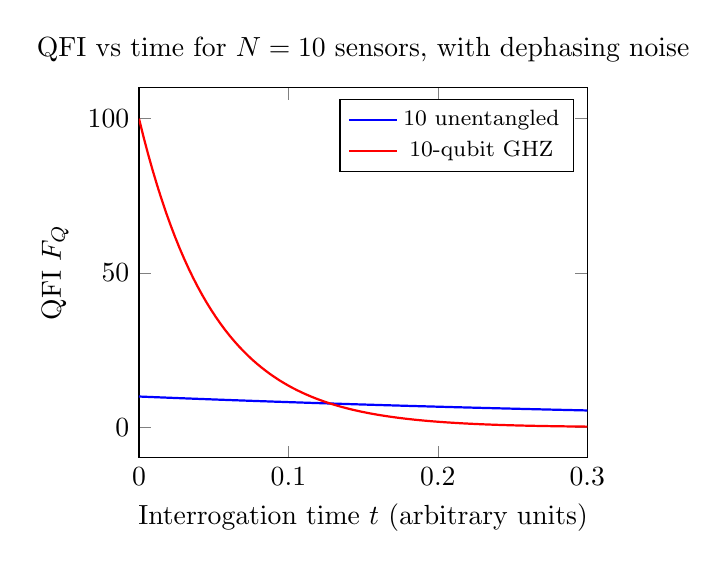
\begin{tikzpicture}

\begin{axis}[width=0.6\textwidth, xlabel={Interrogation time $t$ (arbitrary units)}, ylabel={QFI $F_Q$}, xmin=0, xmax=0.3, legend pos=north east, legend style={font=\footnotesize}, title={QFI vs time for $N=10$ sensors, with dephasing noise}, ylabel style={align=center}]

\addplot[domain=0:0.3, samples=100, thick, blue] {10 * exp(-2 * x)};

\addlegendentry{10 unentangled}

\addplot[domain=0:0.3, samples=100, thick, red] {100 * exp(-20 * x)};

\addlegendentry{10-qubit GHZ}

\end{axis}

\end{tikzpicture}

\caption{Quantum Fisher information as a function of interrogation time $t$ for estimating a phase (or frequency) with $N=10$ two-level systems under dephasing noise (rate $\Gamma=1$ unit). \textcolor{blue}{Blue curve}: $N$ unentangled atoms (each contributes $e^{-2\Gamma t}t^2$ so total $F_Q = 10 t^2 e^{-2t}$ up to units). \textcolor{red}{Red curve}: $N$-atom GHZ state ($F_Q = 100 t^2 e^{-20 t}$). At very short times, the GHZ has higher $F_Q$ (steeper initial rise), but it reaches a peak and then decays much faster. The optimum for GHZ is at a shorter $t$ than for unentangled, and yields here a slightly smaller maximum $F_Q$. In this noise regime, entanglement does not offer a long-term advantage, highlighting the fragility of GHZ states to decoherence.}

\label{fig:GHZ-dephasing}

\end{figure}



Figure \ref{fig:GHZ-dephasing} illustrates this comparison for $N=10$
and $\Gamma=1$ (in arbitrary units). We see that initially the GHZ
curve (red) surpasses the unentangled (blue), but then it drops
sharply. The unentangled $F_Q$ decays more slowly and eventually is
higher for larger $t$. Depending on what interrogation time is used,
one or the other performs better. If one optimizes $t$, the
unentangled scheme achieves a better maximum in this example.



The conclusion is that in presence of uncorrelated decoherence, the
achievable precision often obeys an \textit{effective shot-noise
  limit} even with entanglement \cite{Demkowicz2012}. More entangled
probes do not indefinitely improve the scaling; instead, there is
typically a crossover point beyond which adding more particles (or
photons) while keeping them all entangled hurts the precision due to
noise. For moderate $N$, one may still get some improvement by
entanglement, but the advantage is polynomially or even exponentially
curtailed. Various strategies to combat this involve using partially
entangled states (like spin-squeezed states which achieve $F_Q \propto
N^{\alpha}$ with $\alpha<2$ but are more robust), or employing quantum
error correction during sensing \cite{Dur2014} to actively correct for
decoherence and restore Heisenberg scaling (at the cost of overhead).



\subsection{Decoherence in Optical Interferometry}



A similar story occurs in optical interferometry with loss. If each
photon has probability $\eta$ to survive the interferometer
(transmittance $\eta$, loss $1-\eta$), then for large $N$ photons the
chance that all $N$ survive (which is roughly $\eta^N$) becomes very
small. A NOON state’s useful component is precisely the component
where all $N$ are intact; any loss collapses it. Thus the effective
Fisher information of a NOON state with loss plummets for large
$N$. It has been shown \cite{Demkowicz2012} that for any fixed loss
rate (e.g. each photon has $95\%$ survival), the asymptotic scaling of
any quantum scheme’s precision is at best shot-noise scaling; one can
at most gain a constant factor improvement (the so-called
\emph{Heisenberg limit is elusive} under noise). In practice, for
moderate $N$ (say up to 10 or 20 photons), one could see an advantage,
but not unbounded with $N$. On the other hand, if loss can be reduced
with $N$ or if certain error-correcting codes are used, one might
circumvent this.



In summary, noise and decoherence tend to reduce the quantum Fisher
information. The QCRB with noise may not scale as favorably with $N$
as the noiseless theory would suggest. Nonetheless, the QFI remains a
powerful tool: one can include the noise process in the quantum state
$\rho_\theta$ (by solving the master equation or Kraus maps for
$\rho_\theta$ with noise) and then compute $F_Q$ to know the best
possible precision in that noisy scenario. This can guide the design
of quantum sensors: for example, one might find that for a given $N$,
a certain partially entangled state has a higher $F_Q$ under noise
than the GHZ state does. Or one might find the optimal $N$ or optimal
time to use in an experiment to maximize the information.



\section{Numerical Example: Simulation of QFI Under Noise}
\label{sec:numerics}



As an optional illustration, we can simulate the quantum Fisher
information for a simple system and see the impact of noise
numerically. Consider a single qubit (spin-$\frac{1}{2}$) used to
estimate a rotation angle $\theta$. The qubit starts in state
$|+\rangle = (|0\rangle+|1\rangle)/\sqrt{2}$ (an eigenstate of
$\sigma_x$) at $\theta=0$. The parameter is encoded by a unitary
$U(\theta) = e^{-i \theta \sigma_z/2}$ (rotation about $z$-axis by
angle $\theta$). If there is no noise, the state is
$|\psi(\theta)\rangle = \frac{1}{\sqrt{2}}(|0\rangle +
e^{-i\theta}|1\rangle)$, which is exactly the Ramsey scenario we
described. The QFI for $\theta$ in this pure state can be calculated
from Eq.~\eqref{eq:QFI-pure}, or using the variance picture: here the
generator is $H=\sigma_z/2$ with variance $1/4$ in the $|+\rangle$
state, so $F_Q = 4 \times \frac{1}{4} = 1$. Indeed, one finds $F_Q =
1$ for all $\theta$; hence $\widehat{Var}(\hat{\theta}) \ge 1$ (in radians$^2$)
for one shot, meaning the smallest uncertainty (one standard
deviation) is $1$ rad, which makes sense given a single qubit gives a
binary outcome at best (with many repeats $\sim \frac{1}{\sqrt{M}}$
improvement).



Now, if the qubit suffers dephasing with decoherence factor $c =
e^{-\Gamma t}$ (here $t$ would correspond to $\theta$ if $\theta$
accumulates over time $t$ linearly, but let’s treat $\theta$ as the
small parameter we estimate), the state becomes $\rho(\theta) =
\frac{1}{2}\begin{pmatrix}1 & c e^{-i\theta} \ c e^{i\theta} &
  1\end{pmatrix}$. The QFI we derived earlier for this state is $F_Q =
  c^2$ (assuming $\theta$ small or general $\theta$ since the QFI for
  phase is independent of the phase value). If $c=0.8$ for example,
  $F_Q = 0.64$. This means the best one can do is now
  $\widehat{Var}(\hat{\theta}) \ge 1/0.64 \approx 1.56$ rad$^2$ per shot, a
  larger uncertainty than without dephasing. As $c \to 0$ (complete
  dephasing), $F_Q \to 0$ and you cannot estimate $\theta$ at all
  (indeed the state becomes completely mixed, which contains no
  information about $\theta$).



For a quick numerical simulation, one could randomly sample
measurement outcomes from an optimal measurement and verify the CR
bound. For brevity, we will skip a full Monte Carlo simulation here
and instead outline pseudocode:




\section{Conclusion}




\bibliographystyle{spphys}
\clearemptydoublepage

% chapter 7
\chapter{Machine Learning and Quantum Sensing}
\abstract{This chapter explores data-driven estimation methods, focusing on Bayesian inference and modern machine-learning approaches. It begins by contrasting the frequentist viewpoint (Fisher information and CRBs) with a Bayesian framework that incorporates prior knowledge into sensing problems. Key Bayesian concepts are introduced: using Bayes’ theorem to update a probability distribution over the unknown parameter(s) as measurement data arrives. The text details how quantum measurement outcomes produce likelihood functions, and how sequential updating yields a posterior distribution whose mean and credible intervals quantify uncertainty. Comparison to frequentist bounds is discussed, emphasizing that Bayesian strategies are especially useful in adaptive sensing or when data are scarce. The chapter includes examples of Bayesian quantum sensing: for instance, estimating magnetic fields with an NV-center qubit or calibrating a trapped-ion sensor using prior models.  Practical aspects (e.g. discretizing the parameter space, computing updates) and metrics like posterior variance and information gain are covered. Throughout, illustrative figures and code snippets demonstrate the updating process.}
%\chapter{Bayesian Inference in Quantum Sensing}
\section{Bayes' Theorem and Priors}
\section{Posterior Updating and Filtering}

Bayesian methods incorporate prior knowledge:
\[
p(\theta|x) = \frac{p(x|\theta) p(\theta)}{p(x)},
\]
with
\[
p(x) = \int p(x|\theta) p(\theta) d\theta.
\]

This enables adaptive estimation strategies, quantification of
uncertainty, and credible intervals.

\bibliographystyle{spphys}
\clearemptydoublepage

\chapter{Applications}
\abstract{This  chapter ties together the concepts by working through concrete sensing applications, often via numerical simulation.}
%\chapter{Application: Magnetic Field Sensing}
\section{Introduction}
We can simulate quantum sensors under time-dependent magnetic fields, entanglement, and noise.
\section{Hamiltonian Modeling}
\section{Phase and Frequency Estimation}
\section{Example: Magnetic Field Estimation}

Consider an unknown time-dependent field $B(t)$:
\[
H(t) = \frac{\mu}{2} B(t) \sigma_z.
\]

By evolving the system and applying Bayesian inference to measurement
outcomes, we can estimate $B(t)$ with high precision.

\section{Conclusion}

\bibliographystyle{spphys}

 \bibliographystyle{unsrt}

\chapter{Quantum Control and Error Mitigation in Sensors}
\abstract{ This chapter would cover techniques for actively preserving coherence and suppressing noise in quantum sensors, such as dynamical decoupling, composite pulse sequences, and simple error-correcting protocols.  Including these control methods would deepen the experimental treatment of decoherence from Chapter 5 and teach readers how to extend sensor coherence times in practice.}
%\input{chapter9}
\bibliographystyle{spphys}

 \bibliographystyle{unsrt}

\chapter{Quantum Sensor Networks and Distributed Sensing}
\abstract{This chapter would explore how multiple quantum sensors can be networked or entangled to perform enhanced measurements (e.g. entangled clock networks or magnetometer arrays).  It would review theoretical proposals and early experiments on distributed quantum sensing, addressing how correlations between sensors can improve spatial resolution or differential measurements.  Adding this material builds on the outlook in Chapter 1 and provides a modern perspective on scaling up quantum sensing using many-body resources.}
%\input{chapter10}
\bibliographystyle{spphys}

\bibliographystyle{unsrt}

\clearemptydoublepage
\chapter{Conclusion and Outlook, all}

\abstract{
In the final chapter we summarize the key concepts covered in the book
and reflect on future directions. We discuss the current status of
quantum hardware (superconducting qubits, trapped ions, Rydberg atoms)
and their applicability to quantum sensing.  We outline open
challenges bla bla
}


\backmatter%%%%%%%%%%%%%%%%%%%%%%%%%%%%%%%%%%%%%%%%%%%%%%%%%%%%%%%
%\include{glossary}
%\include{solutions}
\printindex



\end{document}




